%%%%%%%%%%%%%%%%%%%%%%%% editor.tex %%%%%%%%%%%%%%%%%%%%%%%%%%%%%
%
% sample root file for the contributions of a "contributed volume"
%
% Use this file as a template for your own input.
%
%%%%%%%%%%%%%%%%%%%%%%%%%%%%% Springer %%%%%%%%%%%%%%%%%%%%%%%%%%


% RECOMMENDED %%%%%%%%%%%%%%%%%%%%%%%%%%%%%%%%%%%%%%%%%%%%%%%%%%%
\documentclass[graybox, envcountchap, natbib]{svmult}

% choose options for [] as required from the list
% in the Reference Guide

%\usepackage{type1cm}        % activate if the above 3 fonts are 
                             % not available on your system

\usepackage{makeidx}         % allows index generation
\usepackage{graphicx}        % standard LaTeX graphics tool
                             % when including figure files
\usepackage{multicol}        % used for the two-column index
\usepackage[bottom]{footmisc}% places footnotes at page bottom

\usepackage{newtxtext}       % 
\usepackage{newtxmath}       % selects Times Roman as basic font
\usepackage{doi}             % makes hyperlinks out of doi in bib

\usepackage{kantlipsum}
\usepackage{cleveref}
\usepackage{wrapfig}

\let\Bbbk\relax              % MER: Fixes compilation error

% see the list of further useful packages in the Reference Guide
\usepackage{chapterbib}
\input{packages}
\input{commands}
\input{macros}
\makeindex             % used for the subject index
                       % please use the style svind.ist with
                       % your makeindex program

%%%%%%%%%%%%%%%%%%%%%%%%%%%%%%%%%%%%%%%%%%%%%%%%%%%%%%%%%%%%%%%%%

\begin{document}

\frontmatter%%%%%%%%%%%%%%%%%%%%%%%%%%%%%%%%%%%%%%%%%%%%%%%%%%%%%%

\include{dedication}
\include{foreword}
\include{preface}
\include{acknowledgement}

\setcounter{tocdepth}{0}
\tableofcontents
\include{contriblist}
\include{acronym}

\mainmatter%%%%%%%%%%%%%%%%%%%%%%%%%%%%%%%%%%%%%%%%%%%%%%%%%%%%%%%

\graphicspath{{chapters/chp1/graphics/}}


\title{Growth and Remodelling Package in FEniCSx}

\author{Karl Munthe, Henrik Finsberg, Samuel Wall, Joakim Sundnes}

\institute{K. Munthe \at Simula Research Laboratory, Oslo, Norway and \\ Department of Informatics, University of Oslo, Norway, \email{karlfredrik@simula.no}
\and
H. Finsberg \at Simula Research Laboratory, Oslo, Norway
\and
S. Wall \at Simula Research Laboratory, Oslo, Norway
\and
J. Sundnes \at Simula Research Laboratory, Oslo, Norway and \\ Department of Informatics, University of Oslo, Norway}

\maketitle
\abstract{The heart is a dynamic organ that changes its size and shape to regulate its behaviour to the demands of the body, which can change for example through body growth, exercise, the onset of a disease, or taking medication. Different models exist to try to capture various types of cardiac growth as a result of mechanical stimuli. In this manuscript we will present a framework created with FEniCSx that allows one to quickly run simulations of growth and remodelling with different material models and different growth laws. We present some of the simulations and compare them to the relevant literature in the field. \added{All the code can be found at \url{https://github.com/karlfm/Growth-and-Remodeling-in-FEniCSx}}}
\vspace{12pt}
\section{Introduction}
In classical continuum mechanics one normally studies the mechanics of bodies where mass\replaced{, linear momentum, angular momentum, and energy are conserved properties}{is a conserved property conserved property}. This approach has been extremely successful and is the bedrock for traditional engineering disciplines, but it does not accurately capture aspects of how living organisms change with respect to their environment. One of the unique features of biological material is its ability to grow and evolve by adding or removing mass. Understanding how biological matter grows and what drives the growth is important, not only to understand normal growth and development, but also when and how growth may become non-compensatory and drive disease.\par It has been known for a long time that the growth of organs, such as the heart, is regulated at least in part by the forces applied to it \citep{Hsu1968}. This understanding has led to the formulation of growth laws that link growth and remodeling to local stress or strain. \par
In this chapter we will introduce a package written in FEniCSx that allows one to easily model growth and remodelling of biological tissue, with the aim of quickly testing combinations of growth models and material models. Allowing researchers to systematically test combinations of material models and growth tensors will aid in the discovery of more accurate models of growth and remodelling phenomena of biological tissue.
\section{Methods}
\subsection{Growth and Remodeling in Continuum Mechanics}
Consider a solid body that is continuously and smoothly deforming from one configuration to another, and denote the initial configuration (also called the reference configuration) as $\mathcal{M}$ and the current configuration $\mathcal{N}$. We denote a point in $\mathcal{M}$ with uppercase letters $\mathbf{X} = (X, Y, Z)$ and a point in $\mathcal{N}$ with lowercase letters $\mathbf{x} = (x, y, z)$\footnote{Apart from the letters $X$, $Y$, and $Z$, all upper case letters represent tensors.}. A point in $\mathcal{M}$ can be mapped to a point in $\mathcal{N}$ by a motion, $\phi(\mathbf{X}): \mathbf{X} \rightarrow \mathbf{x}$, which is a diffeomorphism. We can map a vector from the reference configuration to the current configuration via the pushforward of $\phi$, which is commonly denoted by $\mathbf{F}$ and is referred to as the deformation gradient, computed as $\mathbf{F} = \partial\mathbf{x}/\partial\mathbf{X}$. The displacement field $\mathbf{u} = \mathbf{x} - \mathbf{X}$ is a vector field describing the displacement of each point $\mathbf{X}$ in the reference configuration to its location $\mathbf{x}$ in the deformed configuration. \par 
Most mechanical models of the heart assume that the tissue is hyperelastic, meaning that deformations of the material conserve its energy, and when any load on the tissue is removed it returns to its original reference shape. Growth, on the other hand, represents a permanent change of the unloaded reference configuration, and cannot be modeled as an elastic deformation. Instead, it is commonly modeled using the framework of plastic or elasto-plastic deformations. The most common framework is to multiplicatively split the deformation tensor into an elastic part and a growth part, 
\begin{equation}
\label{eq: multiplicative split}
    \mathbf{F} = \mathbf{F}_e\mathbf{F}_g,
\end{equation}
where $\mathbf{F}_e$ is the elastic deformation and $\mathbf{F}_g$ is the plastic deformation that represents growth. Among the early adopters of the multiplicative split of elastic and plastic deformations in biological tissue were by \citep{Kondaurov1987}, \citep{Takamizawa1990}, and \citep{Rodriguez1994}. \par 
\added{One interpretation of \ref{eq: multiplicative split} is that the material first deforms by $\mathbf{F}_g$ in a way that does not cause stress, but might cause incompatibilities in the form of discontinuities or overlapping material. The deformation described by $\mathbf{F}_g$ leads to an unphysical intermediate configuration, which is then deformed by $\mathbf{F}_e$} \deleted{Then it deforms by $\mathbf{F}_e$}in a way that removes the unphysical characteristics that occurred from $\mathbf{F}_g$, but adds residual stress. \added{Sufficient conditions for the existence of intermediate configurations such as $\mathbf{F}_g$ are discussed in \citep{Goodbrake2021}}. We assume that the deformation described by $\mathbf{F}_e$ is hyperelastic, such that we can obtain the first Piola–Kirchhoff stress tensor by differentiating a strain energy function,
\begin{equation}
\label{eq: stress}
    \mathbf{P} = \frac{\partial\Psi}{\partial \mathbf{F}_e}.
\end{equation}
The total deformation due to growth is obtained by 
\begin{equation*}
    \mathbf{F}_g^{i + 1} = \mathbf{F}_g^i\mathbf{F}_g^\mathrm{inc},
\end{equation*}
where $\mathbf{F}_g^\mathrm{inc}$ is the incremental growth tensor, and $\mathbf{F}_g^i$ is the cumulative growth that has occurred after $i$ steps. The initial growth tensor, $\mathbf{F}_g^0$, is set to the identity tensor. The reason we have to use this form of the growth tensor is because we are always mapping from the same reference configuration; so after $n$ steps, we are applying $n$ growth deformations, which looks like 
\begin{equation*}
    \mathbf{F}_g^{n} = \mathbf{F}_{g}^\mathrm{inc}\vert_{t=0}\mathbf{F}_{g}^\mathrm{inc}\vert_{t=1} \cdots \mathbf{F}_{g}^\mathrm{inc}\vert_{t=n},
\end{equation*}  
where $\mathbf{F}_{g}^\mathrm{inc}\vert_{t=i}$ means the $\mathbf{F}_{g}^\mathrm{inc}$ at the $i$'th step. Note that the $i$'th incremental growth tensor is dependent on the stress or strain that occurred in the $i-1$'th growth step (see \citep{Goriely2007}). It is common to express the incremental growth tensor in terms of fiber, crossfiber, and normal directions 
\begin{equation*}
    \mathbf{F}_g^\mathrm{inc} = F^\mathrm{inc}_{g,f}\mathbf{e}_f\otimes \mathbf{e}_f + F^\mathrm{inc}_{g,c}\mathbf{e}_c\otimes \mathbf{e}_c + F^\mathrm{inc}_{g,n}\mathbf{e}_n\otimes \mathbf{e}_n.
\end{equation*}
where $F^\mathrm{inc}_{g, i}$ for  $i = \{f, c, n\}$ are functions of either stress or strain, and $\mathbf{e}_i$ for $i = {\{f, c, n\}}$ are orthonormal basis vectors in the fiber, crossfiber, and normal directions respectively. The equations are then furnished with boundary conditions that that describe the load and displacement of the boundary,
\begin{equation} \label{eq: system of equations}
\begin{aligned}
    \mathbf{F} & = \mathbf{F}_e\mathbf{F}_g && \text{in } \mathcal{M} ,\\
    \nabla\cdot\mathbf{P} & = 0 && \text{in } \mathcal{M}, \\
    \mathbf{P}\cdot \nu & = 0 && \text{on } \partial\mathcal{M}_N, \\
    \mathbf{u} & = g_D && \text{on } \partial\mathcal{M}_D,
\end{aligned}
\end{equation} 
where $\nu$ is a surface normal vector, $\partial\mathcal{M}_N$ amd $\partial\mathcal{M}_D$ denote the boundaries which are prescribed Neumann and Dirichlet boundary conditions respectively. Finally, we need to specify the material model, and in this paper we use a \replaced{nearly}{weakly} incompressible neo-Hookean model, so (\ref{eq: stress}) becomes
\begin{align*}
    \mathbf{P} &= \frac{\partial\Psi_\text{iso}}{\partial \mathbf{F}_e} + \frac{\partial\Psi_\text{vol}}{\partial \mathbf{F}_e}, \\
    \mathbf{P} &= \frac{\partial}{\partial \mathbf{F}_e}\left[\frac{\mu}{2}\left(\tr\mathbf{\bar{C}} - 3\right) + \kappa(J-1)^2\right],
\end{align*}
where and $\mu$ and $\kappa$ material parameters. $\Psi_\text{iso}$ and $\Psi_\text{vol}$ are the isochoric (distortional) and volumetric (dilational) parts of the strain energy function. To decouple the energy stored in the body as a result of volume preserving deformation and non-volume preserving deformation, we set $\mathbf{\bar{F}}_e = \mathbf{F}_eJ^{-1/3}$, whose determinant is equal to the identity tensor. The isochoric right Cauchy-Green deformation tensor, $\mathbf{\bar{C}}$, is calculated as $\mathbf{\bar{C}} = \mathbf{\bar{F}}_e^\top \mathbf{\bar{F}}_e$. Now, $\partial\Psi_\text{iso}/\partial \mathbf{F}_e = 0$ only if the deformation preserves the shape, and $\partial\Psi_\text{vol}/\partial \mathbf{F}_e = 0$ only if the deformation preserves the volume (see chapter 6 of \citep{Holzapfel2002} for more details). \par 
For further information about continuum mechanics we recommend \citep{Marsden1983} and \citep{Holzapfel2002}, and for further information about growth and remodelling we recommend \citep{Goriely2017} and \citep{Yavari2010}.

\subsection{Numerical Implementation And Experiments}
 
\added{Algorithm \ref{alg:growth_deform} shows the algorithm used for strain based growth. For stress based growth, you would update the stress tensor rather than the strain tensor, and for additive growth laws, you would add the cumulative and incremental growth tensors instead of multiplying them together.} \par
\begin{algorithm} 
    \caption{Growth tensor and stress/strain tensor are updated at each growth step. Both $\mathbf{F}_\mathrm{e}$ and $\mathbf{F}_g^\mathrm{inc}$ are dependent on $\mathbf{u}$.}\label{alg:growth_deform}
    \SetAlgoLined
    \For{each time step}{
        Solve (\ref{eq: system of equations}) for the displacement $\mathbf{u}$\;
        Update the stress/strain tensor using $\mathbf{u}$ from the previous line.\;
        Update the growth tensor using the stress/strain tensor from the previous line.\;
    }
\end{algorithm} 
\emph{Constructing the weak form}: We multiply $\nabla\cdot\mathbf{P}$ by a test function, which we set to be in the same function space as $\mathbf{u}$, and integrate over a discretization of $\mathcal{M}$. By applying integration by parts, we obtain
\begin{align}
    \label{eq: weak conservation of momentum}
    \int_\Omega(\nabla\cdot\mathbf{P})\cdot\eta d\mathbf{X} &= 0  \notag\\
    \int_\Omega \mathbf{P} : \nabla\eta d\mathbf{X} &= \int_{\partial\Omega}\mathbf{P}\cdot\eta \cdot \nu dA.
\end{align}
\replaced{Since we are using test functions, $\eta$, that vanish on $\partial_D\mathcal{M}$, and the normal component of $\mathbf{P}$ is zero on $\partial_N\mathcal{M}$ we can set the boundary integral to zero. }{Since we are using Dirichlet boundary conditions, $\mathbf{P} = 0$ on the boundary of $\mathcal{N}$}. (\ref{eq: weak conservation of momentum}) is solved using FEniCSx \cite{DOLFINx}. 
\par
\emph{Iteratively solving the conservation of momentum}: We now solve (\ref{eq: weak conservation of momentum}) for the displacement $\mathbf{u}$, which we can use to compute all the necessary variables. \added{We use tetrahedral, second order, continuous, Lagrange elements to approximate $\mathbf{u}$; and a first order, discontinuous, Lagrange elements to approximate $\mathbf{F}_e$ and $\mathbf{F}_g$. This is a common numerical scheme in cardiac mechanics which has been demonstrated to avoid locking \citep{oliveira2016comparison}.} $\mathbf{F}_g$ is initially set to be the identity tensor. \par
\subsection{Solving Growth Laws on the Unit Cube}
\label{subsec: simulations}
In the simulations we have run we have aligned the $x$-axis with the fiber direction and the $y$-, and $z$-axis are the crossfiber and normal direction. To be consistent with the literature we will use $\mathbf{e}_f$, $\mathbf{e}_c$, and $\mathbf{e}_n$ to denote the unit vectors in the $(x, y, z)$ directions respectively.  \par
\emph{Boundary conditions:} We set the following boundary conditions
\begin{align*}
    g_D = \begin{cases}
        u &= \begin{cases}
            0 & \text{on } x = 0, \\
            u_D & \text{on } x = 1,
        \end{cases} \\
        v &= 0 \qquad \ \ \text{on } y = 0, \\
        w &= 0 \qquad \ \ \text{on } z = 0,
    \end{cases}
\end{align*}
where $u$, $v$, and $w$ are the displacement in the $x$, $y$, and $z$ direction respectively. $u_D$ specifies how much the body is displaced. 
\par

\emph{Numerical simulations:} We ran two simulations, one with a 10\% stretch and one with a 10\% compression which corresponds to $u_D = 0.1$ and $u_D = -0.1$ respectively. For the GCG model, $F_{g,c,\mathrm{max}}$ was set to 1.2 in the stretch simulation and 0.8 in the compression simulation (see table \ref{tab:growth models}). We set $\mu = 15$ kPa and $\kappa = 100$ kPa.
\subsection{The different growth models}
\label{sub:different models} 
In this paper we compare five growth models which we have taken from \citep{Taber1998}, \citep{Kroon2009}, \citep{Goktepe}, and \citep{Kerckhoffs2012}. The growth models are given in table \ref{tab:growth models} where LT2 is from \citep{Taber1998}, KFR is from \citep{Kroon2009}, GEG and GCG are from \citep{Goktepe} and KOM is from \citep{Kerckhoffs2012}. Each growth model had a set point that either determined the homeostatic level of stress, stretch, or strain. When the stress, stretch, or strain reaches the set point, then growth will cease to occur. If this does not happen, the body will grow indefinitely, which we call runaway growth. We used the same variables as they were given in the original papers, except for the \replaced{GCG}{$GCG$}, where we scaled the variables to more accurately fit with the shear modulus used here. The values are tabulated in table \ref{tab:parameters}.
%\newgeometry{right=1cm, left=1cm}%,right=1cm,top=1cm,bottom=1cm}
\begin{table}
\centering
\makebox[\textwidth][c]{
\renewcommand{\arraystretch}{4}
\begin{tabular}{|c||c|c|c|}
\hline \hline
 & $F_{g,f}^{i+1}$ & $F_{g,n}^{i+1}$ & $F_{g,c}^{i+1}$ \\
\hline \hline
LT2 & $\displaystyle F_{g,f}^i\left(\frac{\sigma_{\theta p} - \sigma_{p,0}}{T\sigma_{p,0}} + 1\right)$ & $\displaystyle F_{g,n}^i\left(\frac{\sigma_{\theta a} - \sigma_{a,0}}{T\sigma_{a,0}} + 1\right)$ & $\displaystyle 1$ \\
\hline
KFR & $\displaystyle F_{g,f}^i(\beta(\sqrt{2 E_{ff} + 1} - 1 - s_\mathrm{hom}) + 1)^{1/3}$ & $\displaystyle F_{g,n}^i(\beta(\sqrt{2 E_{ff} + 1} - 1 - s_\mathrm{hom}) + 1)^{1/3}$ & $\displaystyle F_{g,c}^i(\beta(\sqrt{2 E_{ff} + 1} - 1 - s_\mathrm{hom}) + 1)^{1/3}$ \\
\hline
GEG & $\displaystyle \frac{1}{\tau}\left(\frac{F_{g,f,\mathrm{max}} - F_{g,f}^i}{F_{g,f,\mathrm{max}} - 1}\right)^\gamma(F_{e, f}^i - \lambda^\text{crit}) + F^i_{g, f}$ & $\displaystyle 1$ & $\displaystyle 1$ \\
\hline
GCG & $\displaystyle 1$ & $\displaystyle  \frac{1}{\tau}\left(\frac{F_{g,c,\mathrm{max}} - F_{g,c}^i}{F_{g,c,\mathrm{max}} - 1}\right)^\gamma(\tr(\mathbf{M}) - p^\mathrm{crit}) + F^i_{g, c}$ & $\displaystyle 1$ \\
\hline
KOM & $\displaystyle \begin{cases}
        F_{g,f}^{i}k_{ff}\frac{f_\mathrm{ff, max}\Delta t_\text{growth}}{1 + \exp(-f_f(s_\mathrm{l}-s_{l,50}))} + 1, \qquad s_\mathrm{l} \geq 0\\
        F_{g,f}^{i}\frac{-f_\mathrm{ff, max}\Delta t_\text{growth}}{1 + \exp(f_f(s_\mathrm{l}+s_{l,50}))} + 1, \qquad s_\mathrm{l} < 0
    \end{cases} $ & $\displaystyle \begin{cases}
        F_{g,c}^{i}\sqrt{k_{cc}\frac{f_{cc,\mathrm{max}}\Delta t_\text{growth}}{1 + \exp(-c_\mathrm{f}(s_\mathrm{t}-s_{t,50}))} + 1}, \qquad s_\mathrm{t} \geq 0\\
        F_{g,c}^{i}\sqrt{\frac{-f_{cc,\mathrm{max}}\Delta t_\text{growth}}{1 + \exp(c_\mathrm{f}(s_\mathrm{t}+s_{t,50}))} + 1}, \qquad s_\mathrm{t} < 0 
    \end{cases} $ & $\displaystyle \begin{cases}
        F_{g,c}^{i}\sqrt{k_{cc}\frac{f_{cc,\mathrm{max}}\Delta t_\text{growth}}{1 + \exp(-c_\mathrm{f}(s_\mathrm{t}-s_{t,50}))} + 1}, \qquad s_\mathrm{t} \geq 0\\
        F_{g,c}^{i}\sqrt{\frac{-f_{cc,\mathrm{max}}\Delta t_\text{growth}}{1 + \exp(c_\mathrm{f}(s_\mathrm{t}+s_{t,50}))} + 1}, \qquad s_\mathrm{t} < 0 
    \end{cases} $ \\
\hline
\end{tabular}
}
\caption{$F_{g,f}$, $F_{g,c}$, $F_{g,n}$,  for each of the five models. The parameters $T$, $\beta$, $\tau$, and $\Delta t$, simply determine the rate of growth and can be tuned to \replaced{match}{math} the growth rate of data obtained from experiments.}
\label{tab:growth models}
\end{table}
%\restoregeometry
\begin{table}[htbp]
    \centering
    \begin{tabular}{|l|l|}
    \hline
    \textbf{Model} & \textbf{Parameters} \\
    \hline
    \textbf{LT2} &   $\sigma_{a,0} = 30$ [kPa], $\sigma_{p,0} = 3$ [kPa], $T = 10^{-4}$ \\ \hline
    \textbf{KFR} &  $s_\mathrm{hom} = 0.13, \beta = 10^{-2}$ \\ \hline
    \textbf{GEG} &  $F_{g,f,\mathrm{max}}=1.5$, $\lambda^\mathrm{crit}=1.01$, $\gamma = 2$, $\tau = 10^2$ \\ \hline
    \textbf{GCG} &  $F_{g,c,\mathrm{max}}=1.2$ and $0.8$,  $p^\mathrm{crit}=0.12, \gamma = 2, \tau = 10^4$ \\ \hline
    \textbf{KOM} &  $f_\mathrm{ff,max} =0.31$ [1/days], $f_f = 150$, $s_{l50} = 0.06$, $F_{ff50} = 1.35$, $f_{l,\mathrm{slope}} = 40$, $f_\mathrm{ff,max} = 0.1$ [1/days] \\
        & $c_\mathrm{f} = 75$, $s_\mathrm{t50} = 0.07$, $F_\mathrm{cc50} = 1.28$, $c_\mathrm{th,slope} = 60$, $E_{ff,\mathrm{set}} = 0$, 
        $E_\mathrm{cross,\mathrm{set}} = 0$, $\Delta t = 10^{-2}$ [days] \\ \hline
    \end{tabular}
    \caption{Model parameters for the growth models. $T$, $\beta$, $\tau$, and $\Delta t$, determine the speed of growth.}
    \label{tab:parameters}
\end{table}
In LT2, $\sigma_{p,0}$ and $\sigma_{a,0}$ are set points for the passive and active fiber stress at equilibrium, and $\sigma_{\theta p}$ and $\sigma_{\theta a}$ are the active and passive fiber stresses. In the simulations we have run, we have only used the passive component of $\sigma$, and have set $\sigma_a = 0$. For KFR, $s_\mathrm{hom}$ is the strain set point. For GEG and GCG, $F_{g,f,\mathrm{max}}$ and $F_{g,c,\mathrm{max}}$ is the maximum amount of growth allowed to occur. $\mathbf{M}$ is the Mandel stress, which is defined as 
\begin{equation*}
    \mathbf{M} = \mathbf{F}^\top \mathbf{P}
\end{equation*}
and $p^\mathrm{crit}$ is the stress set point. $\lambda^\text{crit}$ is the strain set point. For KOM, $k_{ff}$ and $k_{cc}$ are defined as
\begin{align*}
    k_{ff} &= \frac{1}{1 + \exp(f_\text{length,slope}(\mathbf{F}_{g,ff}^i - F_{ff,50}))} \\
    k_{cc} &= \frac{1}{1 + \exp(c_\text{thickness,slope}(\mathbf{F}_{g,cc}^i - F_{cc,50}))}
\end{align*}
and $s_\mathrm{l}$, and $s_\mathrm{t}$ are defined as
\begin{align*}
    s_\mathrm{l} &= \max(E_{ff}) - E_{ff, \mathrm{set}} \\
    s_\mathrm{t} &= \min(E_\text{cross, max}) - E_\mathrm{cross, set}
\end{align*}
where $E_{ij}$ is the Lagrange strain tensor, and $E_{ff}$ is the strain in the fiber direction, and $E_\text{cross, max}$ is the maximum algebraic maximum principle strain of the matrix (see \citep{Witzenburg2018})
\begin{equation*}
    E_\text{cross} = \begin{pmatrix}
        E_{cc} & E_{cr} \\
        E_{rc} & E_{rr}
    \end{pmatrix}
\end{equation*}
and $E_{ff, \mathrm{set}}$ and $E_\mathrm{cross, set}$ are set points. \par
\deleted{In the simulations run, LT2 displayed runaway growth as was also observed in the simulations run in }\citep{Witzenburg2018}. Growth stops for the LT2 model when $\sigma_{\theta} = \sigma_{0}$.
\deleted{which was not satisfied in our simulations or in the simulations run by} \citep{Witzenburg2018}. For KOM, since $k_{cc}$ and $k_{ff}$ are logistic functions, the growth is bounded from above and below inhibiting runaway growth. Finally, for KFR, it does not appear obvious that it will not obtain runaway growth, but other simulations setups that were tested did result in runaway growth, even though the one we present here does not.
\section{Results}
The data we collected from the two simulations (see section \ref{subsec: simulations}) were the the stretch and growth that occurred in the middle of the cube. The results are depicted in figures \ref{fig:10p_stretch} and \ref{fig:10p_compression}. The top row of each figure displays the fiber and crossfiber components of the growth tensor, $\mathbf{F}_g$, and the bottom row displays the fiber and crossfiber components of the elastic deformation tensor $\mathbf{F}_e$. In the simulations we ran, $\mathbf{F}_e$ is diagonal, so the components of $\mathbf{F}_e$ are the principle stretches. This is because $\sqrt{\mathbf{e}_i^\top\mathbf{C}_e\mathbf{e}_i}$ is the principle stretch in the $i$'th direction, and $\sqrt{\mathbf{e}_i^\top\mathbf{C}_e\mathbf{e}_i} = \sqrt{\mathbf{e}_i^\top\mathbf{F}_e^\top\mathbf{F}_e\mathbf{e}_i} = \mathbf{F}_e\mathbf{e}_i$. By the same reasoning, the diagonal components of $\mathbf{F}_g$ (which are the only non-zero components), give the growth in fiber, crossfiber, and normal direction. Increasing $\kappa$ did not yield qualitatively different results. \par
GCG seems to be converging to $F_{g,c,\mathrm{max}}$, and GEG seem to have converged because it reached $\lambda^\text{crit}$. The reason GCG is growing oppositely compared to GEG is probably because GEG was created to model growth triggered by volume overload while GCG was created to capture growth triggered by pressure overload. KFR grew an equal amount in each direction, and stabilized. It is not clear under what conditions KFR should be stable because $s_\mathrm{hom}$ is the same in each direction. When we ran simulations with other boundary conditions, the solution diverged. The KOM model was stable for many different types of boundary conditions, but is the most computationally expensive model to run.\par 
\begin{figure}[h]
    \centering
    \includegraphics[width=\textwidth]{10p_stretch_3.png}
    \caption{Growth and stretch predicted by a 10\% stretch in the fiber direction.}
    \label{fig:10p_stretch}
\end{figure}
\begin{figure}[h]
    \centering
    \includegraphics[width=\textwidth]{10p_compression_3.png}
    \caption{Growth and stretch predicted by a 10\% compression in the fiber direction.}
    \label{fig:10p_compression}
\end{figure}    
\section{Conclusion and future work}
We have implemented a general growth and remodelling framework using the FEniCSx program in Python. The goal is to easily change material models and growth models. This will allow researchers to compare their models with other models in the field. Future work will include implementing more complex geometries, more growth laws, and more material models. \added{The models we have used in this paper are not derived from the dissipation equation but are instead phenomenologically derived growth laws and future work should investigate whether or not they satisfy the laws of thermodynamics. Another avenue of future research we wish to pursue is to look into constrained mixture models which model how changes in the various constituents influence the characteristics of the tissue.} \deleted{Specifically, w}\added{W}e also wish to add models that have more mathematically sophisticated stopping criteria, such as the ones developed by Erlich et al. \citep{Erlich2023} uses an energy penalty to construct a stopping criteria and \citep{Erlich2024} looks into how curvature\footnote{The intrinsic three dimensional curvature, not the two dimensional curvature of the surface of the body.} in the reference configuration could be used as a stopping criteria. Future work will also implement the growth models on geometries with fibers. We tried running the models on various fiber orientations and found them extremely sensitive to fibers that varied throughout the domain. Preliminary results indicate that some of the models do not converge to a steady state for relatively small perturbations of the variables or if the fibers are not well aligned with the body, something we plan on quantifying in the future. \par
When this package is further developed we aim to add it to the Pulse\footnote{https://github.com/finsberg/fenicsx-pulse} package. \par
The models we compared have been developed to capture different aspects of growth and were tuned to be used on different material models, so an apples-to-apples comparison might not be fair. Furthermore, the growth models we have used are not taking into account residual stresses that exist within the material before or after growth occurs. \par
Finally, experimental data is needed to verify which models are accurate or capture the correct phenomena of growing cardiac tissue.
% \newpage
\bibliographystyle{spbasic}
\bibliography{chapters/chp1/bibliography.bib}
% \printbibliography
% \end{document}

\graphicspath{{chapters/chp1/graphics/}}


\title{Growth and Remodelling Package in FEniCSx}

\author{Karl Munthe, Henrik Finsberg, Samuel Wall, Joakim Sundnes}

\institute{K. Munthe \at Simula Research Laboratory, Oslo, Norway and \\ Department of Informatics, University of Oslo, Norway, \email{karlfredrik@simula.no}
\and
H. Finsberg \at Simula Research Laboratory, Oslo, Norway
\and
S. Wall \at Simula Research Laboratory, Oslo, Norway
\and
J. Sundnes \at Simula Research Laboratory, Oslo, Norway and \\ Department of Informatics, University of Oslo, Norway}

\maketitle
\abstract{The heart is a dynamic organ that changes its size and shape to regulate its behaviour to the demands of the body, which can change for example through body growth, exercise, the onset of a disease, or taking medication. Different models exist to try to capture various types of cardiac growth as a result of mechanical stimuli. In this manuscript we will present a framework created with FEniCSx that allows one to quickly run simulations of growth and remodelling with different material models and different growth laws. We present some of the simulations and compare them to the relevant literature in the field. \added{All the code can be found at \url{https://github.com/karlfm/Growth-and-Remodeling-in-FEniCSx}}}
\vspace{12pt}
\section{Introduction}
In classical continuum mechanics one normally studies the mechanics of bodies where mass\replaced{, linear momentum, angular momentum, and energy are conserved properties}{is a conserved property conserved property}. This approach has been extremely successful and is the bedrock for traditional engineering disciplines, but it does not accurately capture aspects of how living organisms change with respect to their environment. One of the unique features of biological material is its ability to grow and evolve by adding or removing mass. Understanding how biological matter grows and what drives the growth is important, not only to understand normal growth and development, but also when and how growth may become non-compensatory and drive disease.\par It has been known for a long time that the growth of organs, such as the heart, is regulated at least in part by the forces applied to it \citep{Hsu1968}. This understanding has led to the formulation of growth laws that link growth and remodeling to local stress or strain. \par
In this chapter we will introduce a package written in FEniCSx that allows one to easily model growth and remodelling of biological tissue, with the aim of quickly testing combinations of growth models and material models. Allowing researchers to systematically test combinations of material models and growth tensors will aid in the discovery of more accurate models of growth and remodelling phenomena of biological tissue.
\section{Methods}
\subsection{Growth and Remodeling in Continuum Mechanics}
Consider a solid body that is continuously and smoothly deforming from one configuration to another, and denote the initial configuration (also called the reference configuration) as $\mathcal{M}$ and the current configuration $\mathcal{N}$. We denote a point in $\mathcal{M}$ with uppercase letters $\mathbf{X} = (X, Y, Z)$ and a point in $\mathcal{N}$ with lowercase letters $\mathbf{x} = (x, y, z)$\footnote{Apart from the letters $X$, $Y$, and $Z$, all upper case letters represent tensors.}. A point in $\mathcal{M}$ can be mapped to a point in $\mathcal{N}$ by a motion, $\phi(\mathbf{X}): \mathbf{X} \rightarrow \mathbf{x}$, which is a diffeomorphism. We can map a vector from the reference configuration to the current configuration via the pushforward of $\phi$, which is commonly denoted by $\mathbf{F}$ and is referred to as the deformation gradient, computed as $\mathbf{F} = \partial\mathbf{x}/\partial\mathbf{X}$. The displacement field $\mathbf{u} = \mathbf{x} - \mathbf{X}$ is a vector field describing the displacement of each point $\mathbf{X}$ in the reference configuration to its location $\mathbf{x}$ in the deformed configuration. \par 
Most mechanical models of the heart assume that the tissue is hyperelastic, meaning that deformations of the material conserve its energy, and when any load on the tissue is removed it returns to its original reference shape. Growth, on the other hand, represents a permanent change of the unloaded reference configuration, and cannot be modeled as an elastic deformation. Instead, it is commonly modeled using the framework of plastic or elasto-plastic deformations. The most common framework is to multiplicatively split the deformation tensor into an elastic part and a growth part, 
\begin{equation}
\label{eq: multiplicative split}
    \mathbf{F} = \mathbf{F}_e\mathbf{F}_g,
\end{equation}
where $\mathbf{F}_e$ is the elastic deformation and $\mathbf{F}_g$ is the plastic deformation that represents growth. Among the early adopters of the multiplicative split of elastic and plastic deformations in biological tissue were by \citep{Kondaurov1987}, \citep{Takamizawa1990}, and \citep{Rodriguez1994}. \par 
\added{One interpretation of \ref{eq: multiplicative split} is that the material first deforms by $\mathbf{F}_g$ in a way that does not cause stress, but might cause incompatibilities in the form of discontinuities or overlapping material. The deformation described by $\mathbf{F}_g$ leads to an unphysical intermediate configuration, which is then deformed by $\mathbf{F}_e$} \deleted{Then it deforms by $\mathbf{F}_e$}in a way that removes the unphysical characteristics that occurred from $\mathbf{F}_g$, but adds residual stress. \added{Sufficient conditions for the existence of intermediate configurations such as $\mathbf{F}_g$ are discussed in \citep{Goodbrake2021}}. We assume that the deformation described by $\mathbf{F}_e$ is hyperelastic, such that we can obtain the first Piola–Kirchhoff stress tensor by differentiating a strain energy function,
\begin{equation}
\label{eq: stress}
    \mathbf{P} = \frac{\partial\Psi}{\partial \mathbf{F}_e}.
\end{equation}
The total deformation due to growth is obtained by 
\begin{equation*}
    \mathbf{F}_g^{i + 1} = \mathbf{F}_g^i\mathbf{F}_g^\mathrm{inc},
\end{equation*}
where $\mathbf{F}_g^\mathrm{inc}$ is the incremental growth tensor, and $\mathbf{F}_g^i$ is the cumulative growth that has occurred after $i$ steps. The initial growth tensor, $\mathbf{F}_g^0$, is set to the identity tensor. The reason we have to use this form of the growth tensor is because we are always mapping from the same reference configuration; so after $n$ steps, we are applying $n$ growth deformations, which looks like 
\begin{equation*}
    \mathbf{F}_g^{n} = \mathbf{F}_{g}^\mathrm{inc}\vert_{t=0}\mathbf{F}_{g}^\mathrm{inc}\vert_{t=1} \cdots \mathbf{F}_{g}^\mathrm{inc}\vert_{t=n},
\end{equation*}  
where $\mathbf{F}_{g}^\mathrm{inc}\vert_{t=i}$ means the $\mathbf{F}_{g}^\mathrm{inc}$ at the $i$'th step. Note that the $i$'th incremental growth tensor is dependent on the stress or strain that occurred in the $i-1$'th growth step (see \citep{Goriely2007}). It is common to express the incremental growth tensor in terms of fiber, crossfiber, and normal directions 
\begin{equation*}
    \mathbf{F}_g^\mathrm{inc} = F^\mathrm{inc}_{g,f}\mathbf{e}_f\otimes \mathbf{e}_f + F^\mathrm{inc}_{g,c}\mathbf{e}_c\otimes \mathbf{e}_c + F^\mathrm{inc}_{g,n}\mathbf{e}_n\otimes \mathbf{e}_n.
\end{equation*}
where $F^\mathrm{inc}_{g, i}$ for  $i = \{f, c, n\}$ are functions of either stress or strain, and $\mathbf{e}_i$ for $i = {\{f, c, n\}}$ are orthonormal basis vectors in the fiber, crossfiber, and normal directions respectively. The equations are then furnished with boundary conditions that that describe the load and displacement of the boundary,
\begin{equation} \label{eq: system of equations}
\begin{aligned}
    \mathbf{F} & = \mathbf{F}_e\mathbf{F}_g && \text{in } \mathcal{M} ,\\
    \nabla\cdot\mathbf{P} & = 0 && \text{in } \mathcal{M}, \\
    \mathbf{P}\cdot \nu & = 0 && \text{on } \partial\mathcal{M}_N, \\
    \mathbf{u} & = g_D && \text{on } \partial\mathcal{M}_D,
\end{aligned}
\end{equation} 
where $\nu$ is a surface normal vector, $\partial\mathcal{M}_N$ amd $\partial\mathcal{M}_D$ denote the boundaries which are prescribed Neumann and Dirichlet boundary conditions respectively. Finally, we need to specify the material model, and in this paper we use a \replaced{nearly}{weakly} incompressible neo-Hookean model, so (\ref{eq: stress}) becomes
\begin{align*}
    \mathbf{P} &= \frac{\partial\Psi_\text{iso}}{\partial \mathbf{F}_e} + \frac{\partial\Psi_\text{vol}}{\partial \mathbf{F}_e}, \\
    \mathbf{P} &= \frac{\partial}{\partial \mathbf{F}_e}\left[\frac{\mu}{2}\left(\tr\mathbf{\bar{C}} - 3\right) + \kappa(J-1)^2\right],
\end{align*}
where and $\mu$ and $\kappa$ material parameters. $\Psi_\text{iso}$ and $\Psi_\text{vol}$ are the isochoric (distortional) and volumetric (dilational) parts of the strain energy function. To decouple the energy stored in the body as a result of volume preserving deformation and non-volume preserving deformation, we set $\mathbf{\bar{F}}_e = \mathbf{F}_eJ^{-1/3}$, whose determinant is equal to the identity tensor. The isochoric right Cauchy-Green deformation tensor, $\mathbf{\bar{C}}$, is calculated as $\mathbf{\bar{C}} = \mathbf{\bar{F}}_e^\top \mathbf{\bar{F}}_e$. Now, $\partial\Psi_\text{iso}/\partial \mathbf{F}_e = 0$ only if the deformation preserves the shape, and $\partial\Psi_\text{vol}/\partial \mathbf{F}_e = 0$ only if the deformation preserves the volume (see chapter 6 of \citep{Holzapfel2002} for more details). \par 
For further information about continuum mechanics we recommend \citep{Marsden1983} and \citep{Holzapfel2002}, and for further information about growth and remodelling we recommend \citep{Goriely2017} and \citep{Yavari2010}.

\subsection{Numerical Implementation And Experiments}
 
\added{Algorithm \ref{alg:growth_deform} shows the algorithm used for strain based growth. For stress based growth, you would update the stress tensor rather than the strain tensor, and for additive growth laws, you would add the cumulative and incremental growth tensors instead of multiplying them together.} \par
\begin{algorithm} 
    \caption{Growth tensor and stress/strain tensor are updated at each growth step. Both $\mathbf{F}_\mathrm{e}$ and $\mathbf{F}_g^\mathrm{inc}$ are dependent on $\mathbf{u}$.}\label{alg:growth_deform}
    \SetAlgoLined
    \For{each time step}{
        Solve (\ref{eq: system of equations}) for the displacement $\mathbf{u}$\;
        Update the stress/strain tensor using $\mathbf{u}$ from the previous line.\;
        Update the growth tensor using the stress/strain tensor from the previous line.\;
    }
\end{algorithm} 
\emph{Constructing the weak form}: We multiply $\nabla\cdot\mathbf{P}$ by a test function, which we set to be in the same function space as $\mathbf{u}$, and integrate over a discretization of $\mathcal{M}$. By applying integration by parts, we obtain
\begin{align}
    \label{eq: weak conservation of momentum}
    \int_\Omega(\nabla\cdot\mathbf{P})\cdot\eta d\mathbf{X} &= 0  \notag\\
    \int_\Omega \mathbf{P} : \nabla\eta d\mathbf{X} &= \int_{\partial\Omega}\mathbf{P}\cdot\eta \cdot \nu dA.
\end{align}
\replaced{Since we are using test functions, $\eta$, that vanish on $\partial_D\mathcal{M}$, and the normal component of $\mathbf{P}$ is zero on $\partial_N\mathcal{M}$ we can set the boundary integral to zero. }{Since we are using Dirichlet boundary conditions, $\mathbf{P} = 0$ on the boundary of $\mathcal{N}$}. (\ref{eq: weak conservation of momentum}) is solved using FEniCSx \cite{DOLFINx}. 
\par
\emph{Iteratively solving the conservation of momentum}: We now solve (\ref{eq: weak conservation of momentum}) for the displacement $\mathbf{u}$, which we can use to compute all the necessary variables. \added{We use tetrahedral, second order, continuous, Lagrange elements to approximate $\mathbf{u}$; and a first order, discontinuous, Lagrange elements to approximate $\mathbf{F}_e$ and $\mathbf{F}_g$. This is a common numerical scheme in cardiac mechanics which has been demonstrated to avoid locking \citep{oliveira2016comparison}.} $\mathbf{F}_g$ is initially set to be the identity tensor. \par
\subsection{Solving Growth Laws on the Unit Cube}
\label{subsec: simulations}
In the simulations we have run we have aligned the $x$-axis with the fiber direction and the $y$-, and $z$-axis are the crossfiber and normal direction. To be consistent with the literature we will use $\mathbf{e}_f$, $\mathbf{e}_c$, and $\mathbf{e}_n$ to denote the unit vectors in the $(x, y, z)$ directions respectively.  \par
\emph{Boundary conditions:} We set the following boundary conditions
\begin{align*}
    g_D = \begin{cases}
        u &= \begin{cases}
            0 & \text{on } x = 0, \\
            u_D & \text{on } x = 1,
        \end{cases} \\
        v &= 0 \qquad \ \ \text{on } y = 0, \\
        w &= 0 \qquad \ \ \text{on } z = 0,
    \end{cases}
\end{align*}
where $u$, $v$, and $w$ are the displacement in the $x$, $y$, and $z$ direction respectively. $u_D$ specifies how much the body is displaced. 
\par

\emph{Numerical simulations:} We ran two simulations, one with a 10\% stretch and one with a 10\% compression which corresponds to $u_D = 0.1$ and $u_D = -0.1$ respectively. For the GCG model, $F_{g,c,\mathrm{max}}$ was set to 1.2 in the stretch simulation and 0.8 in the compression simulation (see table \ref{tab:growth models}). We set $\mu = 15$ kPa and $\kappa = 100$ kPa.
\subsection{The different growth models}
\label{sub:different models} 
In this paper we compare five growth models which we have taken from \citep{Taber1998}, \citep{Kroon2009}, \citep{Goktepe}, and \citep{Kerckhoffs2012}. The growth models are given in table \ref{tab:growth models} where LT2 is from \citep{Taber1998}, KFR is from \citep{Kroon2009}, GEG and GCG are from \citep{Goktepe} and KOM is from \citep{Kerckhoffs2012}. Each growth model had a set point that either determined the homeostatic level of stress, stretch, or strain. When the stress, stretch, or strain reaches the set point, then growth will cease to occur. If this does not happen, the body will grow indefinitely, which we call runaway growth. We used the same variables as they were given in the original papers, except for the \replaced{GCG}{$GCG$}, where we scaled the variables to more accurately fit with the shear modulus used here. The values are tabulated in table \ref{tab:parameters}.
%\newgeometry{right=1cm, left=1cm}%,right=1cm,top=1cm,bottom=1cm}
\begin{table}
\centering
\makebox[\textwidth][c]{
\renewcommand{\arraystretch}{4}
\begin{tabular}{|c||c|c|c|}
\hline \hline
 & $F_{g,f}^{i+1}$ & $F_{g,n}^{i+1}$ & $F_{g,c}^{i+1}$ \\
\hline \hline
LT2 & $\displaystyle F_{g,f}^i\left(\frac{\sigma_{\theta p} - \sigma_{p,0}}{T\sigma_{p,0}} + 1\right)$ & $\displaystyle F_{g,n}^i\left(\frac{\sigma_{\theta a} - \sigma_{a,0}}{T\sigma_{a,0}} + 1\right)$ & $\displaystyle 1$ \\
\hline
KFR & $\displaystyle F_{g,f}^i(\beta(\sqrt{2 E_{ff} + 1} - 1 - s_\mathrm{hom}) + 1)^{1/3}$ & $\displaystyle F_{g,n}^i(\beta(\sqrt{2 E_{ff} + 1} - 1 - s_\mathrm{hom}) + 1)^{1/3}$ & $\displaystyle F_{g,c}^i(\beta(\sqrt{2 E_{ff} + 1} - 1 - s_\mathrm{hom}) + 1)^{1/3}$ \\
\hline
GEG & $\displaystyle \frac{1}{\tau}\left(\frac{F_{g,f,\mathrm{max}} - F_{g,f}^i}{F_{g,f,\mathrm{max}} - 1}\right)^\gamma(F_{e, f}^i - \lambda^\text{crit}) + F^i_{g, f}$ & $\displaystyle 1$ & $\displaystyle 1$ \\
\hline
GCG & $\displaystyle 1$ & $\displaystyle  \frac{1}{\tau}\left(\frac{F_{g,c,\mathrm{max}} - F_{g,c}^i}{F_{g,c,\mathrm{max}} - 1}\right)^\gamma(\tr(\mathbf{M}) - p^\mathrm{crit}) + F^i_{g, c}$ & $\displaystyle 1$ \\
\hline
KOM & $\displaystyle \begin{cases}
        F_{g,f}^{i}k_{ff}\frac{f_\mathrm{ff, max}\Delta t_\text{growth}}{1 + \exp(-f_f(s_\mathrm{l}-s_{l,50}))} + 1, \qquad s_\mathrm{l} \geq 0\\
        F_{g,f}^{i}\frac{-f_\mathrm{ff, max}\Delta t_\text{growth}}{1 + \exp(f_f(s_\mathrm{l}+s_{l,50}))} + 1, \qquad s_\mathrm{l} < 0
    \end{cases} $ & $\displaystyle \begin{cases}
        F_{g,c}^{i}\sqrt{k_{cc}\frac{f_{cc,\mathrm{max}}\Delta t_\text{growth}}{1 + \exp(-c_\mathrm{f}(s_\mathrm{t}-s_{t,50}))} + 1}, \qquad s_\mathrm{t} \geq 0\\
        F_{g,c}^{i}\sqrt{\frac{-f_{cc,\mathrm{max}}\Delta t_\text{growth}}{1 + \exp(c_\mathrm{f}(s_\mathrm{t}+s_{t,50}))} + 1}, \qquad s_\mathrm{t} < 0 
    \end{cases} $ & $\displaystyle \begin{cases}
        F_{g,c}^{i}\sqrt{k_{cc}\frac{f_{cc,\mathrm{max}}\Delta t_\text{growth}}{1 + \exp(-c_\mathrm{f}(s_\mathrm{t}-s_{t,50}))} + 1}, \qquad s_\mathrm{t} \geq 0\\
        F_{g,c}^{i}\sqrt{\frac{-f_{cc,\mathrm{max}}\Delta t_\text{growth}}{1 + \exp(c_\mathrm{f}(s_\mathrm{t}+s_{t,50}))} + 1}, \qquad s_\mathrm{t} < 0 
    \end{cases} $ \\
\hline
\end{tabular}
}
\caption{$F_{g,f}$, $F_{g,c}$, $F_{g,n}$,  for each of the five models. The parameters $T$, $\beta$, $\tau$, and $\Delta t$, simply determine the rate of growth and can be tuned to \replaced{match}{math} the growth rate of data obtained from experiments.}
\label{tab:growth models}
\end{table}
%\restoregeometry
\begin{table}[htbp]
    \centering
    \begin{tabular}{|l|l|}
    \hline
    \textbf{Model} & \textbf{Parameters} \\
    \hline
    \textbf{LT2} &   $\sigma_{a,0} = 30$ [kPa], $\sigma_{p,0} = 3$ [kPa], $T = 10^{-4}$ \\ \hline
    \textbf{KFR} &  $s_\mathrm{hom} = 0.13, \beta = 10^{-2}$ \\ \hline
    \textbf{GEG} &  $F_{g,f,\mathrm{max}}=1.5$, $\lambda^\mathrm{crit}=1.01$, $\gamma = 2$, $\tau = 10^2$ \\ \hline
    \textbf{GCG} &  $F_{g,c,\mathrm{max}}=1.2$ and $0.8$,  $p^\mathrm{crit}=0.12, \gamma = 2, \tau = 10^4$ \\ \hline
    \textbf{KOM} &  $f_\mathrm{ff,max} =0.31$ [1/days], $f_f = 150$, $s_{l50} = 0.06$, $F_{ff50} = 1.35$, $f_{l,\mathrm{slope}} = 40$, $f_\mathrm{ff,max} = 0.1$ [1/days] \\
        & $c_\mathrm{f} = 75$, $s_\mathrm{t50} = 0.07$, $F_\mathrm{cc50} = 1.28$, $c_\mathrm{th,slope} = 60$, $E_{ff,\mathrm{set}} = 0$, 
        $E_\mathrm{cross,\mathrm{set}} = 0$, $\Delta t = 10^{-2}$ [days] \\ \hline
    \end{tabular}
    \caption{Model parameters for the growth models. $T$, $\beta$, $\tau$, and $\Delta t$, determine the speed of growth.}
    \label{tab:parameters}
\end{table}
In LT2, $\sigma_{p,0}$ and $\sigma_{a,0}$ are set points for the passive and active fiber stress at equilibrium, and $\sigma_{\theta p}$ and $\sigma_{\theta a}$ are the active and passive fiber stresses. In the simulations we have run, we have only used the passive component of $\sigma$, and have set $\sigma_a = 0$. For KFR, $s_\mathrm{hom}$ is the strain set point. For GEG and GCG, $F_{g,f,\mathrm{max}}$ and $F_{g,c,\mathrm{max}}$ is the maximum amount of growth allowed to occur. $\mathbf{M}$ is the Mandel stress, which is defined as 
\begin{equation*}
    \mathbf{M} = \mathbf{F}^\top \mathbf{P}
\end{equation*}
and $p^\mathrm{crit}$ is the stress set point. $\lambda^\text{crit}$ is the strain set point. For KOM, $k_{ff}$ and $k_{cc}$ are defined as
\begin{align*}
    k_{ff} &= \frac{1}{1 + \exp(f_\text{length,slope}(\mathbf{F}_{g,ff}^i - F_{ff,50}))} \\
    k_{cc} &= \frac{1}{1 + \exp(c_\text{thickness,slope}(\mathbf{F}_{g,cc}^i - F_{cc,50}))}
\end{align*}
and $s_\mathrm{l}$, and $s_\mathrm{t}$ are defined as
\begin{align*}
    s_\mathrm{l} &= \max(E_{ff}) - E_{ff, \mathrm{set}} \\
    s_\mathrm{t} &= \min(E_\text{cross, max}) - E_\mathrm{cross, set}
\end{align*}
where $E_{ij}$ is the Lagrange strain tensor, and $E_{ff}$ is the strain in the fiber direction, and $E_\text{cross, max}$ is the maximum algebraic maximum principle strain of the matrix (see \citep{Witzenburg2018})
\begin{equation*}
    E_\text{cross} = \begin{pmatrix}
        E_{cc} & E_{cr} \\
        E_{rc} & E_{rr}
    \end{pmatrix}
\end{equation*}
and $E_{ff, \mathrm{set}}$ and $E_\mathrm{cross, set}$ are set points. \par
\deleted{In the simulations run, LT2 displayed runaway growth as was also observed in the simulations run in }\citep{Witzenburg2018}. Growth stops for the LT2 model when $\sigma_{\theta} = \sigma_{0}$.
\deleted{which was not satisfied in our simulations or in the simulations run by} \citep{Witzenburg2018}. For KOM, since $k_{cc}$ and $k_{ff}$ are logistic functions, the growth is bounded from above and below inhibiting runaway growth. Finally, for KFR, it does not appear obvious that it will not obtain runaway growth, but other simulations setups that were tested did result in runaway growth, even though the one we present here does not.
\section{Results}
The data we collected from the two simulations (see section \ref{subsec: simulations}) were the the stretch and growth that occurred in the middle of the cube. The results are depicted in figures \ref{fig:10p_stretch} and \ref{fig:10p_compression}. The top row of each figure displays the fiber and crossfiber components of the growth tensor, $\mathbf{F}_g$, and the bottom row displays the fiber and crossfiber components of the elastic deformation tensor $\mathbf{F}_e$. In the simulations we ran, $\mathbf{F}_e$ is diagonal, so the components of $\mathbf{F}_e$ are the principle stretches. This is because $\sqrt{\mathbf{e}_i^\top\mathbf{C}_e\mathbf{e}_i}$ is the principle stretch in the $i$'th direction, and $\sqrt{\mathbf{e}_i^\top\mathbf{C}_e\mathbf{e}_i} = \sqrt{\mathbf{e}_i^\top\mathbf{F}_e^\top\mathbf{F}_e\mathbf{e}_i} = \mathbf{F}_e\mathbf{e}_i$. By the same reasoning, the diagonal components of $\mathbf{F}_g$ (which are the only non-zero components), give the growth in fiber, crossfiber, and normal direction. Increasing $\kappa$ did not yield qualitatively different results. \par
GCG seems to be converging to $F_{g,c,\mathrm{max}}$, and GEG seem to have converged because it reached $\lambda^\text{crit}$. The reason GCG is growing oppositely compared to GEG is probably because GEG was created to model growth triggered by volume overload while GCG was created to capture growth triggered by pressure overload. KFR grew an equal amount in each direction, and stabilized. It is not clear under what conditions KFR should be stable because $s_\mathrm{hom}$ is the same in each direction. When we ran simulations with other boundary conditions, the solution diverged. The KOM model was stable for many different types of boundary conditions, but is the most computationally expensive model to run.\par 
\begin{figure}[h]
    \centering
    \includegraphics[width=\textwidth]{10p_stretch_3.png}
    \caption{Growth and stretch predicted by a 10\% stretch in the fiber direction.}
    \label{fig:10p_stretch}
\end{figure}
\begin{figure}[h]
    \centering
    \includegraphics[width=\textwidth]{10p_compression_3.png}
    \caption{Growth and stretch predicted by a 10\% compression in the fiber direction.}
    \label{fig:10p_compression}
\end{figure}    
\section{Conclusion and future work}
We have implemented a general growth and remodelling framework using the FEniCSx program in Python. The goal is to easily change material models and growth models. This will allow researchers to compare their models with other models in the field. Future work will include implementing more complex geometries, more growth laws, and more material models. \added{The models we have used in this paper are not derived from the dissipation equation but are instead phenomenologically derived growth laws and future work should investigate whether or not they satisfy the laws of thermodynamics. Another avenue of future research we wish to pursue is to look into constrained mixture models which model how changes in the various constituents influence the characteristics of the tissue.} \deleted{Specifically, w}\added{W}e also wish to add models that have more mathematically sophisticated stopping criteria, such as the ones developed by Erlich et al. \citep{Erlich2023} uses an energy penalty to construct a stopping criteria and \citep{Erlich2024} looks into how curvature\footnote{The intrinsic three dimensional curvature, not the two dimensional curvature of the surface of the body.} in the reference configuration could be used as a stopping criteria. Future work will also implement the growth models on geometries with fibers. We tried running the models on various fiber orientations and found them extremely sensitive to fibers that varied throughout the domain. Preliminary results indicate that some of the models do not converge to a steady state for relatively small perturbations of the variables or if the fibers are not well aligned with the body, something we plan on quantifying in the future. \par
When this package is further developed we aim to add it to the Pulse\footnote{https://github.com/finsberg/fenicsx-pulse} package. \par
The models we compared have been developed to capture different aspects of growth and were tuned to be used on different material models, so an apples-to-apples comparison might not be fair. Furthermore, the growth models we have used are not taking into account residual stresses that exist within the material before or after growth occurs. \par
Finally, experimental data is needed to verify which models are accurate or capture the correct phenomena of growing cardiac tissue.
% \newpage
\bibliographystyle{spbasic}
\bibliography{chapters/chp1/bibliography.bib}
% \printbibliography
% \end{document}
 
\graphicspath{{chapters/chp1/graphics/}}


\title{Growth and Remodelling Package in FEniCSx}

\author{Karl Munthe, Henrik Finsberg, Samuel Wall, Joakim Sundnes}

\institute{K. Munthe \at Simula Research Laboratory, Oslo, Norway and \\ Department of Informatics, University of Oslo, Norway, \email{karlfredrik@simula.no}
\and
H. Finsberg \at Simula Research Laboratory, Oslo, Norway
\and
S. Wall \at Simula Research Laboratory, Oslo, Norway
\and
J. Sundnes \at Simula Research Laboratory, Oslo, Norway and \\ Department of Informatics, University of Oslo, Norway}

\maketitle
\abstract{The heart is a dynamic organ that changes its size and shape to regulate its behaviour to the demands of the body, which can change for example through body growth, exercise, the onset of a disease, or taking medication. Different models exist to try to capture various types of cardiac growth as a result of mechanical stimuli. In this manuscript we will present a framework created with FEniCSx that allows one to quickly run simulations of growth and remodelling with different material models and different growth laws. We present some of the simulations and compare them to the relevant literature in the field. \added{All the code can be found at \url{https://github.com/karlfm/Growth-and-Remodeling-in-FEniCSx}}}
\vspace{12pt}
\section{Introduction}
In classical continuum mechanics one normally studies the mechanics of bodies where mass\replaced{, linear momentum, angular momentum, and energy are conserved properties}{is a conserved property conserved property}. This approach has been extremely successful and is the bedrock for traditional engineering disciplines, but it does not accurately capture aspects of how living organisms change with respect to their environment. One of the unique features of biological material is its ability to grow and evolve by adding or removing mass. Understanding how biological matter grows and what drives the growth is important, not only to understand normal growth and development, but also when and how growth may become non-compensatory and drive disease.\par It has been known for a long time that the growth of organs, such as the heart, is regulated at least in part by the forces applied to it \citep{Hsu1968}. This understanding has led to the formulation of growth laws that link growth and remodeling to local stress or strain. \par
In this chapter we will introduce a package written in FEniCSx that allows one to easily model growth and remodelling of biological tissue, with the aim of quickly testing combinations of growth models and material models. Allowing researchers to systematically test combinations of material models and growth tensors will aid in the discovery of more accurate models of growth and remodelling phenomena of biological tissue.
\section{Methods}
\subsection{Growth and Remodeling in Continuum Mechanics}
Consider a solid body that is continuously and smoothly deforming from one configuration to another, and denote the initial configuration (also called the reference configuration) as $\mathcal{M}$ and the current configuration $\mathcal{N}$. We denote a point in $\mathcal{M}$ with uppercase letters $\mathbf{X} = (X, Y, Z)$ and a point in $\mathcal{N}$ with lowercase letters $\mathbf{x} = (x, y, z)$\footnote{Apart from the letters $X$, $Y$, and $Z$, all upper case letters represent tensors.}. A point in $\mathcal{M}$ can be mapped to a point in $\mathcal{N}$ by a motion, $\phi(\mathbf{X}): \mathbf{X} \rightarrow \mathbf{x}$, which is a diffeomorphism. We can map a vector from the reference configuration to the current configuration via the pushforward of $\phi$, which is commonly denoted by $\mathbf{F}$ and is referred to as the deformation gradient, computed as $\mathbf{F} = \partial\mathbf{x}/\partial\mathbf{X}$. The displacement field $\mathbf{u} = \mathbf{x} - \mathbf{X}$ is a vector field describing the displacement of each point $\mathbf{X}$ in the reference configuration to its location $\mathbf{x}$ in the deformed configuration. \par 
Most mechanical models of the heart assume that the tissue is hyperelastic, meaning that deformations of the material conserve its energy, and when any load on the tissue is removed it returns to its original reference shape. Growth, on the other hand, represents a permanent change of the unloaded reference configuration, and cannot be modeled as an elastic deformation. Instead, it is commonly modeled using the framework of plastic or elasto-plastic deformations. The most common framework is to multiplicatively split the deformation tensor into an elastic part and a growth part, 
\begin{equation}
\label{eq: multiplicative split}
    \mathbf{F} = \mathbf{F}_e\mathbf{F}_g,
\end{equation}
where $\mathbf{F}_e$ is the elastic deformation and $\mathbf{F}_g$ is the plastic deformation that represents growth. Among the early adopters of the multiplicative split of elastic and plastic deformations in biological tissue were by \citep{Kondaurov1987}, \citep{Takamizawa1990}, and \citep{Rodriguez1994}. \par 
\added{One interpretation of \ref{eq: multiplicative split} is that the material first deforms by $\mathbf{F}_g$ in a way that does not cause stress, but might cause incompatibilities in the form of discontinuities or overlapping material. The deformation described by $\mathbf{F}_g$ leads to an unphysical intermediate configuration, which is then deformed by $\mathbf{F}_e$} \deleted{Then it deforms by $\mathbf{F}_e$}in a way that removes the unphysical characteristics that occurred from $\mathbf{F}_g$, but adds residual stress. \added{Sufficient conditions for the existence of intermediate configurations such as $\mathbf{F}_g$ are discussed in \citep{Goodbrake2021}}. We assume that the deformation described by $\mathbf{F}_e$ is hyperelastic, such that we can obtain the first Piola–Kirchhoff stress tensor by differentiating a strain energy function,
\begin{equation}
\label{eq: stress}
    \mathbf{P} = \frac{\partial\Psi}{\partial \mathbf{F}_e}.
\end{equation}
The total deformation due to growth is obtained by 
\begin{equation*}
    \mathbf{F}_g^{i + 1} = \mathbf{F}_g^i\mathbf{F}_g^\mathrm{inc},
\end{equation*}
where $\mathbf{F}_g^\mathrm{inc}$ is the incremental growth tensor, and $\mathbf{F}_g^i$ is the cumulative growth that has occurred after $i$ steps. The initial growth tensor, $\mathbf{F}_g^0$, is set to the identity tensor. The reason we have to use this form of the growth tensor is because we are always mapping from the same reference configuration; so after $n$ steps, we are applying $n$ growth deformations, which looks like 
\begin{equation*}
    \mathbf{F}_g^{n} = \mathbf{F}_{g}^\mathrm{inc}\vert_{t=0}\mathbf{F}_{g}^\mathrm{inc}\vert_{t=1} \cdots \mathbf{F}_{g}^\mathrm{inc}\vert_{t=n},
\end{equation*}  
where $\mathbf{F}_{g}^\mathrm{inc}\vert_{t=i}$ means the $\mathbf{F}_{g}^\mathrm{inc}$ at the $i$'th step. Note that the $i$'th incremental growth tensor is dependent on the stress or strain that occurred in the $i-1$'th growth step (see \citep{Goriely2007}). It is common to express the incremental growth tensor in terms of fiber, crossfiber, and normal directions 
\begin{equation*}
    \mathbf{F}_g^\mathrm{inc} = F^\mathrm{inc}_{g,f}\mathbf{e}_f\otimes \mathbf{e}_f + F^\mathrm{inc}_{g,c}\mathbf{e}_c\otimes \mathbf{e}_c + F^\mathrm{inc}_{g,n}\mathbf{e}_n\otimes \mathbf{e}_n.
\end{equation*}
where $F^\mathrm{inc}_{g, i}$ for  $i = \{f, c, n\}$ are functions of either stress or strain, and $\mathbf{e}_i$ for $i = {\{f, c, n\}}$ are orthonormal basis vectors in the fiber, crossfiber, and normal directions respectively. The equations are then furnished with boundary conditions that that describe the load and displacement of the boundary,
\begin{equation} \label{eq: system of equations}
\begin{aligned}
    \mathbf{F} & = \mathbf{F}_e\mathbf{F}_g && \text{in } \mathcal{M} ,\\
    \nabla\cdot\mathbf{P} & = 0 && \text{in } \mathcal{M}, \\
    \mathbf{P}\cdot \nu & = 0 && \text{on } \partial\mathcal{M}_N, \\
    \mathbf{u} & = g_D && \text{on } \partial\mathcal{M}_D,
\end{aligned}
\end{equation} 
where $\nu$ is a surface normal vector, $\partial\mathcal{M}_N$ amd $\partial\mathcal{M}_D$ denote the boundaries which are prescribed Neumann and Dirichlet boundary conditions respectively. Finally, we need to specify the material model, and in this paper we use a \replaced{nearly}{weakly} incompressible neo-Hookean model, so (\ref{eq: stress}) becomes
\begin{align*}
    \mathbf{P} &= \frac{\partial\Psi_\text{iso}}{\partial \mathbf{F}_e} + \frac{\partial\Psi_\text{vol}}{\partial \mathbf{F}_e}, \\
    \mathbf{P} &= \frac{\partial}{\partial \mathbf{F}_e}\left[\frac{\mu}{2}\left(\tr\mathbf{\bar{C}} - 3\right) + \kappa(J-1)^2\right],
\end{align*}
where and $\mu$ and $\kappa$ material parameters. $\Psi_\text{iso}$ and $\Psi_\text{vol}$ are the isochoric (distortional) and volumetric (dilational) parts of the strain energy function. To decouple the energy stored in the body as a result of volume preserving deformation and non-volume preserving deformation, we set $\mathbf{\bar{F}}_e = \mathbf{F}_eJ^{-1/3}$, whose determinant is equal to the identity tensor. The isochoric right Cauchy-Green deformation tensor, $\mathbf{\bar{C}}$, is calculated as $\mathbf{\bar{C}} = \mathbf{\bar{F}}_e^\top \mathbf{\bar{F}}_e$. Now, $\partial\Psi_\text{iso}/\partial \mathbf{F}_e = 0$ only if the deformation preserves the shape, and $\partial\Psi_\text{vol}/\partial \mathbf{F}_e = 0$ only if the deformation preserves the volume (see chapter 6 of \citep{Holzapfel2002} for more details). \par 
For further information about continuum mechanics we recommend \citep{Marsden1983} and \citep{Holzapfel2002}, and for further information about growth and remodelling we recommend \citep{Goriely2017} and \citep{Yavari2010}.

\subsection{Numerical Implementation And Experiments}
 
\added{Algorithm \ref{alg:growth_deform} shows the algorithm used for strain based growth. For stress based growth, you would update the stress tensor rather than the strain tensor, and for additive growth laws, you would add the cumulative and incremental growth tensors instead of multiplying them together.} \par
\begin{algorithm} 
    \caption{Growth tensor and stress/strain tensor are updated at each growth step. Both $\mathbf{F}_\mathrm{e}$ and $\mathbf{F}_g^\mathrm{inc}$ are dependent on $\mathbf{u}$.}\label{alg:growth_deform}
    \SetAlgoLined
    \For{each time step}{
        Solve (\ref{eq: system of equations}) for the displacement $\mathbf{u}$\;
        Update the stress/strain tensor using $\mathbf{u}$ from the previous line.\;
        Update the growth tensor using the stress/strain tensor from the previous line.\;
    }
\end{algorithm} 
\emph{Constructing the weak form}: We multiply $\nabla\cdot\mathbf{P}$ by a test function, which we set to be in the same function space as $\mathbf{u}$, and integrate over a discretization of $\mathcal{M}$. By applying integration by parts, we obtain
\begin{align}
    \label{eq: weak conservation of momentum}
    \int_\Omega(\nabla\cdot\mathbf{P})\cdot\eta d\mathbf{X} &= 0  \notag\\
    \int_\Omega \mathbf{P} : \nabla\eta d\mathbf{X} &= \int_{\partial\Omega}\mathbf{P}\cdot\eta \cdot \nu dA.
\end{align}
\replaced{Since we are using test functions, $\eta$, that vanish on $\partial_D\mathcal{M}$, and the normal component of $\mathbf{P}$ is zero on $\partial_N\mathcal{M}$ we can set the boundary integral to zero. }{Since we are using Dirichlet boundary conditions, $\mathbf{P} = 0$ on the boundary of $\mathcal{N}$}. (\ref{eq: weak conservation of momentum}) is solved using FEniCSx \cite{DOLFINx}. 
\par
\emph{Iteratively solving the conservation of momentum}: We now solve (\ref{eq: weak conservation of momentum}) for the displacement $\mathbf{u}$, which we can use to compute all the necessary variables. \added{We use tetrahedral, second order, continuous, Lagrange elements to approximate $\mathbf{u}$; and a first order, discontinuous, Lagrange elements to approximate $\mathbf{F}_e$ and $\mathbf{F}_g$. This is a common numerical scheme in cardiac mechanics which has been demonstrated to avoid locking \citep{oliveira2016comparison}.} $\mathbf{F}_g$ is initially set to be the identity tensor. \par
\subsection{Solving Growth Laws on the Unit Cube}
\label{subsec: simulations}
In the simulations we have run we have aligned the $x$-axis with the fiber direction and the $y$-, and $z$-axis are the crossfiber and normal direction. To be consistent with the literature we will use $\mathbf{e}_f$, $\mathbf{e}_c$, and $\mathbf{e}_n$ to denote the unit vectors in the $(x, y, z)$ directions respectively.  \par
\emph{Boundary conditions:} We set the following boundary conditions
\begin{align*}
    g_D = \begin{cases}
        u &= \begin{cases}
            0 & \text{on } x = 0, \\
            u_D & \text{on } x = 1,
        \end{cases} \\
        v &= 0 \qquad \ \ \text{on } y = 0, \\
        w &= 0 \qquad \ \ \text{on } z = 0,
    \end{cases}
\end{align*}
where $u$, $v$, and $w$ are the displacement in the $x$, $y$, and $z$ direction respectively. $u_D$ specifies how much the body is displaced. 
\par

\emph{Numerical simulations:} We ran two simulations, one with a 10\% stretch and one with a 10\% compression which corresponds to $u_D = 0.1$ and $u_D = -0.1$ respectively. For the GCG model, $F_{g,c,\mathrm{max}}$ was set to 1.2 in the stretch simulation and 0.8 in the compression simulation (see table \ref{tab:growth models}). We set $\mu = 15$ kPa and $\kappa = 100$ kPa.
\subsection{The different growth models}
\label{sub:different models} 
In this paper we compare five growth models which we have taken from \citep{Taber1998}, \citep{Kroon2009}, \citep{Goktepe}, and \citep{Kerckhoffs2012}. The growth models are given in table \ref{tab:growth models} where LT2 is from \citep{Taber1998}, KFR is from \citep{Kroon2009}, GEG and GCG are from \citep{Goktepe} and KOM is from \citep{Kerckhoffs2012}. Each growth model had a set point that either determined the homeostatic level of stress, stretch, or strain. When the stress, stretch, or strain reaches the set point, then growth will cease to occur. If this does not happen, the body will grow indefinitely, which we call runaway growth. We used the same variables as they were given in the original papers, except for the \replaced{GCG}{$GCG$}, where we scaled the variables to more accurately fit with the shear modulus used here. The values are tabulated in table \ref{tab:parameters}.
%\newgeometry{right=1cm, left=1cm}%,right=1cm,top=1cm,bottom=1cm}
\begin{table}
\centering
\makebox[\textwidth][c]{
\renewcommand{\arraystretch}{4}
\begin{tabular}{|c||c|c|c|}
\hline \hline
 & $F_{g,f}^{i+1}$ & $F_{g,n}^{i+1}$ & $F_{g,c}^{i+1}$ \\
\hline \hline
LT2 & $\displaystyle F_{g,f}^i\left(\frac{\sigma_{\theta p} - \sigma_{p,0}}{T\sigma_{p,0}} + 1\right)$ & $\displaystyle F_{g,n}^i\left(\frac{\sigma_{\theta a} - \sigma_{a,0}}{T\sigma_{a,0}} + 1\right)$ & $\displaystyle 1$ \\
\hline
KFR & $\displaystyle F_{g,f}^i(\beta(\sqrt{2 E_{ff} + 1} - 1 - s_\mathrm{hom}) + 1)^{1/3}$ & $\displaystyle F_{g,n}^i(\beta(\sqrt{2 E_{ff} + 1} - 1 - s_\mathrm{hom}) + 1)^{1/3}$ & $\displaystyle F_{g,c}^i(\beta(\sqrt{2 E_{ff} + 1} - 1 - s_\mathrm{hom}) + 1)^{1/3}$ \\
\hline
GEG & $\displaystyle \frac{1}{\tau}\left(\frac{F_{g,f,\mathrm{max}} - F_{g,f}^i}{F_{g,f,\mathrm{max}} - 1}\right)^\gamma(F_{e, f}^i - \lambda^\text{crit}) + F^i_{g, f}$ & $\displaystyle 1$ & $\displaystyle 1$ \\
\hline
GCG & $\displaystyle 1$ & $\displaystyle  \frac{1}{\tau}\left(\frac{F_{g,c,\mathrm{max}} - F_{g,c}^i}{F_{g,c,\mathrm{max}} - 1}\right)^\gamma(\tr(\mathbf{M}) - p^\mathrm{crit}) + F^i_{g, c}$ & $\displaystyle 1$ \\
\hline
KOM & $\displaystyle \begin{cases}
        F_{g,f}^{i}k_{ff}\frac{f_\mathrm{ff, max}\Delta t_\text{growth}}{1 + \exp(-f_f(s_\mathrm{l}-s_{l,50}))} + 1, \qquad s_\mathrm{l} \geq 0\\
        F_{g,f}^{i}\frac{-f_\mathrm{ff, max}\Delta t_\text{growth}}{1 + \exp(f_f(s_\mathrm{l}+s_{l,50}))} + 1, \qquad s_\mathrm{l} < 0
    \end{cases} $ & $\displaystyle \begin{cases}
        F_{g,c}^{i}\sqrt{k_{cc}\frac{f_{cc,\mathrm{max}}\Delta t_\text{growth}}{1 + \exp(-c_\mathrm{f}(s_\mathrm{t}-s_{t,50}))} + 1}, \qquad s_\mathrm{t} \geq 0\\
        F_{g,c}^{i}\sqrt{\frac{-f_{cc,\mathrm{max}}\Delta t_\text{growth}}{1 + \exp(c_\mathrm{f}(s_\mathrm{t}+s_{t,50}))} + 1}, \qquad s_\mathrm{t} < 0 
    \end{cases} $ & $\displaystyle \begin{cases}
        F_{g,c}^{i}\sqrt{k_{cc}\frac{f_{cc,\mathrm{max}}\Delta t_\text{growth}}{1 + \exp(-c_\mathrm{f}(s_\mathrm{t}-s_{t,50}))} + 1}, \qquad s_\mathrm{t} \geq 0\\
        F_{g,c}^{i}\sqrt{\frac{-f_{cc,\mathrm{max}}\Delta t_\text{growth}}{1 + \exp(c_\mathrm{f}(s_\mathrm{t}+s_{t,50}))} + 1}, \qquad s_\mathrm{t} < 0 
    \end{cases} $ \\
\hline
\end{tabular}
}
\caption{$F_{g,f}$, $F_{g,c}$, $F_{g,n}$,  for each of the five models. The parameters $T$, $\beta$, $\tau$, and $\Delta t$, simply determine the rate of growth and can be tuned to \replaced{match}{math} the growth rate of data obtained from experiments.}
\label{tab:growth models}
\end{table}
%\restoregeometry
\begin{table}[htbp]
    \centering
    \begin{tabular}{|l|l|}
    \hline
    \textbf{Model} & \textbf{Parameters} \\
    \hline
    \textbf{LT2} &   $\sigma_{a,0} = 30$ [kPa], $\sigma_{p,0} = 3$ [kPa], $T = 10^{-4}$ \\ \hline
    \textbf{KFR} &  $s_\mathrm{hom} = 0.13, \beta = 10^{-2}$ \\ \hline
    \textbf{GEG} &  $F_{g,f,\mathrm{max}}=1.5$, $\lambda^\mathrm{crit}=1.01$, $\gamma = 2$, $\tau = 10^2$ \\ \hline
    \textbf{GCG} &  $F_{g,c,\mathrm{max}}=1.2$ and $0.8$,  $p^\mathrm{crit}=0.12, \gamma = 2, \tau = 10^4$ \\ \hline
    \textbf{KOM} &  $f_\mathrm{ff,max} =0.31$ [1/days], $f_f = 150$, $s_{l50} = 0.06$, $F_{ff50} = 1.35$, $f_{l,\mathrm{slope}} = 40$, $f_\mathrm{ff,max} = 0.1$ [1/days] \\
        & $c_\mathrm{f} = 75$, $s_\mathrm{t50} = 0.07$, $F_\mathrm{cc50} = 1.28$, $c_\mathrm{th,slope} = 60$, $E_{ff,\mathrm{set}} = 0$, 
        $E_\mathrm{cross,\mathrm{set}} = 0$, $\Delta t = 10^{-2}$ [days] \\ \hline
    \end{tabular}
    \caption{Model parameters for the growth models. $T$, $\beta$, $\tau$, and $\Delta t$, determine the speed of growth.}
    \label{tab:parameters}
\end{table}
In LT2, $\sigma_{p,0}$ and $\sigma_{a,0}$ are set points for the passive and active fiber stress at equilibrium, and $\sigma_{\theta p}$ and $\sigma_{\theta a}$ are the active and passive fiber stresses. In the simulations we have run, we have only used the passive component of $\sigma$, and have set $\sigma_a = 0$. For KFR, $s_\mathrm{hom}$ is the strain set point. For GEG and GCG, $F_{g,f,\mathrm{max}}$ and $F_{g,c,\mathrm{max}}$ is the maximum amount of growth allowed to occur. $\mathbf{M}$ is the Mandel stress, which is defined as 
\begin{equation*}
    \mathbf{M} = \mathbf{F}^\top \mathbf{P}
\end{equation*}
and $p^\mathrm{crit}$ is the stress set point. $\lambda^\text{crit}$ is the strain set point. For KOM, $k_{ff}$ and $k_{cc}$ are defined as
\begin{align*}
    k_{ff} &= \frac{1}{1 + \exp(f_\text{length,slope}(\mathbf{F}_{g,ff}^i - F_{ff,50}))} \\
    k_{cc} &= \frac{1}{1 + \exp(c_\text{thickness,slope}(\mathbf{F}_{g,cc}^i - F_{cc,50}))}
\end{align*}
and $s_\mathrm{l}$, and $s_\mathrm{t}$ are defined as
\begin{align*}
    s_\mathrm{l} &= \max(E_{ff}) - E_{ff, \mathrm{set}} \\
    s_\mathrm{t} &= \min(E_\text{cross, max}) - E_\mathrm{cross, set}
\end{align*}
where $E_{ij}$ is the Lagrange strain tensor, and $E_{ff}$ is the strain in the fiber direction, and $E_\text{cross, max}$ is the maximum algebraic maximum principle strain of the matrix (see \citep{Witzenburg2018})
\begin{equation*}
    E_\text{cross} = \begin{pmatrix}
        E_{cc} & E_{cr} \\
        E_{rc} & E_{rr}
    \end{pmatrix}
\end{equation*}
and $E_{ff, \mathrm{set}}$ and $E_\mathrm{cross, set}$ are set points. \par
\deleted{In the simulations run, LT2 displayed runaway growth as was also observed in the simulations run in }\citep{Witzenburg2018}. Growth stops for the LT2 model when $\sigma_{\theta} = \sigma_{0}$.
\deleted{which was not satisfied in our simulations or in the simulations run by} \citep{Witzenburg2018}. For KOM, since $k_{cc}$ and $k_{ff}$ are logistic functions, the growth is bounded from above and below inhibiting runaway growth. Finally, for KFR, it does not appear obvious that it will not obtain runaway growth, but other simulations setups that were tested did result in runaway growth, even though the one we present here does not.
\section{Results}
The data we collected from the two simulations (see section \ref{subsec: simulations}) were the the stretch and growth that occurred in the middle of the cube. The results are depicted in figures \ref{fig:10p_stretch} and \ref{fig:10p_compression}. The top row of each figure displays the fiber and crossfiber components of the growth tensor, $\mathbf{F}_g$, and the bottom row displays the fiber and crossfiber components of the elastic deformation tensor $\mathbf{F}_e$. In the simulations we ran, $\mathbf{F}_e$ is diagonal, so the components of $\mathbf{F}_e$ are the principle stretches. This is because $\sqrt{\mathbf{e}_i^\top\mathbf{C}_e\mathbf{e}_i}$ is the principle stretch in the $i$'th direction, and $\sqrt{\mathbf{e}_i^\top\mathbf{C}_e\mathbf{e}_i} = \sqrt{\mathbf{e}_i^\top\mathbf{F}_e^\top\mathbf{F}_e\mathbf{e}_i} = \mathbf{F}_e\mathbf{e}_i$. By the same reasoning, the diagonal components of $\mathbf{F}_g$ (which are the only non-zero components), give the growth in fiber, crossfiber, and normal direction. Increasing $\kappa$ did not yield qualitatively different results. \par
GCG seems to be converging to $F_{g,c,\mathrm{max}}$, and GEG seem to have converged because it reached $\lambda^\text{crit}$. The reason GCG is growing oppositely compared to GEG is probably because GEG was created to model growth triggered by volume overload while GCG was created to capture growth triggered by pressure overload. KFR grew an equal amount in each direction, and stabilized. It is not clear under what conditions KFR should be stable because $s_\mathrm{hom}$ is the same in each direction. When we ran simulations with other boundary conditions, the solution diverged. The KOM model was stable for many different types of boundary conditions, but is the most computationally expensive model to run.\par 
\begin{figure}[h]
    \centering
    \includegraphics[width=\textwidth]{10p_stretch_3.png}
    \caption{Growth and stretch predicted by a 10\% stretch in the fiber direction.}
    \label{fig:10p_stretch}
\end{figure}
\begin{figure}[h]
    \centering
    \includegraphics[width=\textwidth]{10p_compression_3.png}
    \caption{Growth and stretch predicted by a 10\% compression in the fiber direction.}
    \label{fig:10p_compression}
\end{figure}    
\section{Conclusion and future work}
We have implemented a general growth and remodelling framework using the FEniCSx program in Python. The goal is to easily change material models and growth models. This will allow researchers to compare their models with other models in the field. Future work will include implementing more complex geometries, more growth laws, and more material models. \added{The models we have used in this paper are not derived from the dissipation equation but are instead phenomenologically derived growth laws and future work should investigate whether or not they satisfy the laws of thermodynamics. Another avenue of future research we wish to pursue is to look into constrained mixture models which model how changes in the various constituents influence the characteristics of the tissue.} \deleted{Specifically, w}\added{W}e also wish to add models that have more mathematically sophisticated stopping criteria, such as the ones developed by Erlich et al. \citep{Erlich2023} uses an energy penalty to construct a stopping criteria and \citep{Erlich2024} looks into how curvature\footnote{The intrinsic three dimensional curvature, not the two dimensional curvature of the surface of the body.} in the reference configuration could be used as a stopping criteria. Future work will also implement the growth models on geometries with fibers. We tried running the models on various fiber orientations and found them extremely sensitive to fibers that varied throughout the domain. Preliminary results indicate that some of the models do not converge to a steady state for relatively small perturbations of the variables or if the fibers are not well aligned with the body, something we plan on quantifying in the future. \par
When this package is further developed we aim to add it to the Pulse\footnote{https://github.com/finsberg/fenicsx-pulse} package. \par
The models we compared have been developed to capture different aspects of growth and were tuned to be used on different material models, so an apples-to-apples comparison might not be fair. Furthermore, the growth models we have used are not taking into account residual stresses that exist within the material before or after growth occurs. \par
Finally, experimental data is needed to verify which models are accurate or capture the correct phenomena of growing cardiac tissue.
% \newpage
\bibliographystyle{spbasic}
\bibliography{chapters/chp1/bibliography.bib}
% \printbibliography
% \end{document}

% Write the full path to the location of the graphics relative to book.tex
\graphicspath{{chapters/marcibal/graphics/}} 

\title{Implementation of the Lam--Bremhorst \texorpdfstring{\(k\)-\(\varepsilon\)}{k-e} turbulence model in FEniCS}
\titlerunning{Implementation of the \texorpdfstring{\(k\)-\(\varepsilon\)}{k-e} turbulence model}

\author{Juraj Marcibál, Hans Joachim Schroll}
\authorrunning{J.~Marcibál, H.~J.~Schroll}

\institute{
J.~Marcibál \email{juraj.marcibal@gmail.com},
H.~J.~Schroll \email{achim@imada.dk} 
\at University of Southern Denmark, Department of Mathematics and Computer Science
}

\maketitle

% ---- Article starts here ---- 

% Abstract
\abstract{
In this paper, we give an overview of turbulence modeling and turbulence in general, followed by an implementation of the Lam--Bremhorst \(k\)-\(\varepsilon\) turbulence model in FEniCS \citep{alnaes2015fenics,baratta2023dolfinx}. We demonstrate how the model can be easily implemented in the latest version of FEniCS, even when working with the simplest methods and schemes. We hope this paper serves as a valuable resource for researchers and enthusiasts seeking a straightforward introduction to turbulence modeling and a practical guide for implementing models in FEniCS.
}

% Section 1 - Introduction
\section{Introduction and governing equations}

Turbulence is an ever-present phenomenon encountered in both natural environments and engineering systems, from airflow over an airplane wing to the movement of water in rivers. It occurs when fluid moves chaotically, irregularly and at a high Reynolds number, presenting challenges for study and applications \citep{wilcox_turbulence_2006}. 

\subsection{Literature review}

Turbulence modeling, including the \(k\)-\(\varepsilon\) model and implementation in FEniCS and other open-source software, has been covered in the literature before. The article by \cite{valen_implementing_2013} implements the model by \citep{launder_application_1974}, which is often regarded as the standard \(k\)-\(\varepsilon\) model, in FEniCS, providing an accessible introduction to turbulence modeling and FEniCS itself. However, the provided code is now over a decade old and only covers a simple channel flow case. 

On the other hand, \cite{mortensen_fenics-based_2011} present a more comprehensive turbulence modeling framework, implementing multiple models, including the Launder-Sharma \(k\)-\(\varepsilon\) model. While it extends beyond the turbulent channel flow example, the code is also incompatible with the latest version of Legacy FEniCS and its complexity makes it less approachable for newcomers.

This article aims to address the need for a clear up-to-date turbulence model implementation in the Legacy FEniCS. We demonstrate that implementing a turbulence model in the latest version is feasible, and satisfactory results can be obtained even when working with simple numerical schemes and simpler turbulence model. Additionally, we provide an introduction to turbulence and turbulence modeling, making this work a valuable starting point for researchers entering the field. 

\subsection{Modeling turbulence}

Consider the incompressible Navier--Stokes (NS) equations
\begin{equation}\label{eq: NS}
    \begin{split}
        \frac{\partial \mathbf{u}}{\partial t} + \mathbf{u} \cdot \nabla{\mathbf{u}}
        = 
        - \frac{1}{\rho} \nabla p + \nabla \cdot (\nu \nabla \mathbf{u}) + \mathbf{f},
        \\
        \nabla \cdot \mathbf{u}
        = 0,
    \end{split}
\end{equation}
where \(\mathbf{u}\), \(p\) are the instantaneous velocity and pressure, \(\mathbf{f}\) represents the external forces, \(\rho\) is the density and \(\nu\) is the molecular viscosity of the fluid. It is well known that solving Equation \eqref{eq: NS} numerically becomes difficult as Reynolds Number gets large. To accurately predict turbulent flow, we either need to work with a very fine mesh and small step-size, or resort to modeling. The former is often not feasible without a large computational power.

One approach to modeling turbulence is to consider not the instantaneous \(\mathbf{u}\) and \(p\), but rather the mean values \(\langle \mathbf{u} \rangle\) and \( \langle p \rangle\). By decomposing \(\mathbf{u}\) and \(p\) into their mean and fluctuating parts \(\mathbf{u} = \langle \mathbf{u} \rangle + \mathbf{u}'\) and \(p = \langle p \rangle + p'\), one can derive governing equations for the mean quantities. Such equations are called the Reynolds-Averaged Navier--Stokes (RANS) equations, and they take the form
\begin{equation}\label{eq: RANS}
    \begin{split}
        \frac{\partial \langle \mathbf{u} \rangle}{\partial t} + \langle \mathbf{u} \rangle \cdot \nabla{\langle \mathbf{u} \rangle}
        = 
        -\frac{1}{\rho} \nabla \langle p \rangle + \nabla \cdot (\nu \nabla \langle \mathbf{u} \rangle ) + \langle \mathbf{f} \rangle - \nabla \cdot \langle \mathbf{u}' \otimes \mathbf{u}' \rangle,
        \\
        \nabla \cdot \langle \mathbf{u} \rangle 
        = 0,
    \end{split}
\end{equation}
where \(\mathbf{R} := - \langle \mathbf{u}' \otimes \mathbf{u}' \rangle\) is the Reynolds stress tensor, often interpreted as describing the effect of turbulence on the mean flow \citep{wilcox_turbulence_2006}. It contains \(\mathbf{u}'\) which is not known nor solved for. The RANS equations are therefore not closed and \(\mathbf{R}\) needs to be modeled, usually using the hypothesis proposed by \cite{boussinesq__essai_1877}:
\begin{equation}\label{eq: Boussinesq hypothesis}
    \mathbf{R} 
    \approx 
    - \frac{2}{3}k \mathbf{I} 
    + \nu_t \left(\nabla{\mathbf{u}} 
    + (\nabla{\mathbf{u}})^T\right)
    \implies
    \nabla \cdot \mathbf{R} 
    \approx
    - \frac{2}{3} \nabla k 
    + \nabla \cdot \left( \nu_t \nabla \mathbf{u} \right),
\end{equation}
where \(\nu_t\) is the turbulent viscosity and \(k\) is the turbulent kinetic energy. Modeling turbulence now reduces to modeling \(\nu_t\) and \(k\), usually by solving additional transport equation or equations, one of them typically being a transport equation for \(k\).

\subsection{The Lam--Bremhorst \(k\)-\(\varepsilon\) model and boundary conditions}

The Lam--Bremhorst (LB) \(k\)-\(\varepsilon\) model \citep{lam_modified_1981} is one of the models proposed to close the RANS equations. It was chosen for its relative simplicity compared to the more popular models such as the model by \cite{launder_application_1974}. Formulated in Equation \eqref{eq: k-eps}, it supplements Equations \eqref{eq: RANS}, \eqref{eq: Boussinesq hypothesis} with two additional transport equations governing \(k\) and \(\varepsilon\) (dissipation of \(k\)). Together, these equations form a closed system that describes the mean behavior of turbulent flow.
\begin{equation}\label{eq: k-eps}
    \begin{split}
        &\frac{\partial \mathbf{u}}{\partial t} 
        + \mathbf{u} \cdot \nabla{\mathbf{u}}
        = 
        - \nabla{\left( \frac{1}{\rho}p + \frac{2}{3}k \right)}
        + \nabla \cdot \left[ (\nu + \nu_t) \nabla \mathbf{u} \right]
        + \mathbf{f},
        \\
        &\nabla \cdot \mathbf{u}
        = 0,
        \\
        &\frac{\partial k}{\partial t} 
        + \mathbf{u} \cdot \nabla{k}
        = \nabla \cdot \left[\left(\nu + \frac{\nu_t}{\sigma_k}\right) \nabla{k} \right]
        + P_k
        - \gamma k,
        \\
        &\frac{\partial \varepsilon}{\partial t} 
        + \mathbf{u} \cdot \nabla{\varepsilon}
        = \nabla \cdot \left[\left(\nu + \frac{\nu_t}{\sigma_\varepsilon}\right) \nabla{\varepsilon}\right]
        + C_1 f_1 P_k \gamma
        - C_2 f_2 \gamma \varepsilon,
        \\
        &\nu_t
        = C_\nu f_\nu \frac{k^2}{\varepsilon},
        \quad 
        P_k 
        = \mathbf{R} : \frac{1}{2} \left(\nabla{\mathbf{u}} + (\nabla{\mathbf{u}})^T\right),
        \quad
        \gamma
        = \frac{\varepsilon}{k},
        \\
        &f_\nu
        = (1 - \exp{\left( -0.0165 \text{Re}_k \right)})^2 \left(1 + \frac{20.5}{\text{Re}_\ell}\right),
        \quad
        f_1
        = 1 + \left( \frac{0.05}{f_\nu}\right)^3,
        \\
        &f_2 
        = 1 - \exp{\left(-\text{Re}_\ell^2\right)},
        \quad
        \text{Re}_k 
        = \frac{\sqrt{k} y}{\nu}, 
        \quad
        \text{Re}_\ell
        = \frac{k^2}{\nu \varepsilon},
        \\
        &C_\nu = 0.09, \quad
        C_1 = 1.44, \quad
        C_2 = 1.92, \quad
        \sigma_k = 1.0, \quad
        \sigma_\varepsilon = 1.3.
    \end{split}
\end{equation}
In Equation \eqref{eq: k-eps}, \(\mathbf{u}\) and \(p\) are the mean velocity and pressure (for better readability we no longer denote averages with \(\langle \cdot \rangle\)), \(k\) and \(\varepsilon\) are the turbulent kinetic energy and its dissipation, \(\rho\), \(\nu\) and \(\mathbf{f}\) are as in Equation \eqref{eq: NS}. Additionally, \(\nu_t\) is the turbulent viscosity, \(P_k\) and \(\gamma\) are the production and reaction terms of \(k\). 

On top of that \(f_\nu\), \(f_1\) and \(f_2\) are the damping functions, which solve the models' inability to predict flow near the wall \citep{greenshields_notes_2022}. Terms \(\text{Re}_k\) and \(\text{Re}_\ell\) are both referred to as the turbulent Reynolds numbers and \(y\) denotes the distance to the nearest solid wall. Lastly, \(C_\nu\), \(C_1\), \(C_2\) and \(\sigma_1\), \(\sigma_2\) are the experimentally determined model constants.

Since RANS and the NS are the same equations with different total pressure and total viscosity terms, they also have similar boundary conditions, hence we will only focus on boundary conditions for the equations governing \(k\) and \(\varepsilon\).

For \(k\) and \(\varepsilon\) consider the domain boundary \(\partial \Omega\) divided into disjoint subboundaries corresponding to solid walls, inflow and outflow. Natural boundary conditions for the outflow for both \(k\) and \(\varepsilon\) are the zero Neumann boundary conditions, i.e. \(\nabla k \cdot \mathbf{n} = 0\) and \(\nabla \varepsilon \cdot \mathbf{n} = 0\). For the solid wall \(k\) is set to zero, the boundary conditions for \(\varepsilon\) differs with different turbulence model, for the LB \(k\)-\(\varepsilon\) model we have \(\nabla \varepsilon \cdot \mathbf{n} = 0\). The inflow boundary conditions are most often estimated from the physical definitions of \(k\) and \(\varepsilon\):
\begin{equation*}\label{eq: definitions of k-e}
    k = \frac{3}{2} (U I)^2, 
    \quad
    \varepsilon = C_\nu \frac{k^{3/2}}{\ell},
\end{equation*}
where \(U\) is the average velocity magnitude, \(I\) is the turbulent intensity and \(\ell\) is the turbulent length scale. Both \(I\) and \(\ell\) are generally not known beforehand and need to be estimated. For estimation of \(I\) and \(\ell\) see \cite{greenshields_notes_2022}. These can then be implemented as Dirichlet boundary conditions in Legacy FEniCS.

\subsection{Non-dimensionalized quantities and the Law of the wall}

In turbulence modeling, many results are formulated using the non-dimensionalized velocity magnitude (\(U^+\)), distance to the wall (\(y^+\)) and turbulent kinetic energy (\(k^+\)) given by:
\begin{equation}\label{eq: non-dimensionalized variables}
    U^+ := \frac{U}{U_\tau},
    \quad
    y^+ := \frac{y U_\tau}{\nu},
    \quad
    k^+ := \frac{k}{U_\tau^2},
\end{equation}
where \(U_\tau := \sqrt{\tau_\text{w}}\) is the so-called friction velocity and \(\tau_\text{w}\) is the so-called wall shear stress, in \(2\)D it is given by \( \tau_\text{w} := \left. \nu [\nabla (\mathbf{u} \cdot \mathbf{t})] \cdot \mathbf{n} \right\rvert_\text{wall} \), where \(\mathbf{n}\) and \(\mathbf{t}\) are the unit outward-facing normal and unit tangent vectors respectively. Note that in \(3\)D the definition of \(\tau_\text{w}\) is more complicated because of non-uniqueness of a tangent vector to the wall. We will however keep the test cases in this paper to \(2\)D only.

% Section 2 - Implementation
\section{Implementation}

In this section, we focus on the implementation of the LB \(k\)-\(\varepsilon\) model. We only outline the implementation of the transport equations for \(k\) and \(\varepsilon\), since the RANS equations can be solved using the same techniques as NS. In our case we used Chorin's splitting method together with Taylor-Hood elements to solve the transient version of RANS equations. For the steady state version, Picard iteration was used. 

\subsection{Weak formulation of the \texorpdfstring{\(k\)-\(\varepsilon\)}{k-e} transport equations}

To derive the weak formulation for the \(k\) equation, we first approximate the temporal derivative \(\partial k / \partial t\) by its finite difference approximation. The entire equation is then multiplied by a test function \(\varphi\). Lastly, the divergence theorem is applied to the diffusion term and zero Neumann boundary conditions are considered, resulting in Equation \eqref{eq: Transport equation for k}. The weak formulation then reads: at each time step \(n+1\) find \(k^{n+1} \in V_{k,\triangle} \subseteq V_k = H^1(\Omega)\) such that:
\begin{equation}\label{eq: Transport equation for k}
    \begin{split}
        &\int_{\Omega} \frac{k^{n+1} - k^n}{\Delta t} \varphi \dx 
        + \int_{\Omega} \left( \mathbf{u}^{n+1} \cdot \Grad k^{n+1} \right) \varphi \dx
        \\
        =
        - &\int_{\Omega} \left( \nu + \frac{\nu_t}{\sigma_k}\right) \Grad k^{n+1} \cdot \Grad \varphi \dx 
        + \int_{\Omega} P_k \varphi \dx 
        - \int_{\Omega} \gamma k^{n+1} \varphi \dx,
    \end{split}
\end{equation}
where \(V_{k, \triangle}\) is the finite element subspace of \(V_k\). The same can be performed for the \(\varepsilon\) transport equation. Both \(V_{k, \triangle}\) and \(V_{\varepsilon, \triangle}\) are spaces of piece-wise linear functions.

Terms \(\nu_t\), \(P_k\), \(\gamma\) and \(f_\nu, f_1, f_2\) are all sources of both non-linearity and coupling, as they all depend on both \(k\) and \(\varepsilon\). If we want to solve the equations separately, using linear solvers, it is most natural to treat all the terms above explicitly, i.e. to compute them using values from the previous time-step. 

\subsection{Further treatment of the equations}

As physical quantities, \(k\) and \(\varepsilon\) only attain positive values. However, the equations as of right now might produce negative values for both. The natural solution is to bound them from below by a small constant \citep{lew_note_2001}. To prevent instabilities, it is also advised to limit \(f_\nu\) to its physical bounds \citep{schimdt_two-equation_1988}:
\begin{equation*}\label{eq: Physical bound of fnu}
    f_\nu \longrightarrow \min(\max(0.01116225, f_\nu), 1.0).
\end{equation*}
It has been observed that the effect of \(k\) in the total pressure term is negligible when compared to the effect of pressure \(p\) or the viscous effects \citep{Ansys_Best_Practice}. On top of that, implementing the \(\nabla k\) term in the RANS equations often leads to instabilities. We therefore decided to omit the \(k\) term altogether from \(\mathbf{R}\):
\begin{equation*}\label{eq: Removing k from R}
    \mathbf{R} \longrightarrow \nu_t \left( \Grad \langle u \rangle + \left( \Grad \langle u \rangle \right)^T \right).
\end{equation*}
This results in a formulation which closer resembles ones found in the literature, as seen in articles by \cite{valen_implementing_2013} or \cite{greenshields_notes_2022}.

\subsection{Computational mesh and distance from the wall}

The \(k\)-\(\varepsilon\) model, as formulated in this article, solves the governing equations up to the solid walls. As we will see in the Results section, the turbulent quantities \(k\) and \(\varepsilon\) display large sensitivity and fluctuations in this region, especially in the region where the value of \(y^+\) is less than \(5\) (called the viscous sub-layer). It is essential that this behavior is captured by the model, therefore a mesh fine enough is required. 

Given a desired non-dimensionalized value \(d^+\), we can construct a mesh, such that for each element that lies on the solid wall, the non-dimensionalized distance \(y^+\) between the wall and the furthest point from the wall in the element is less than \(d^+\), by computing the actual distance \(y\) from Equation \eqref{eq: non-dimensionalized variables}. The problem is that the wall shear stress \(\tau_\text{w}\), used in Equation \eqref{eq: non-dimensionalized variables}, is in general not known beforehand and must be estimated. In short, for a pressure-driven turbulent flow, the wall shear stress can be estimated by plugging the solution for Hagen-Poiseuille flow into the definition of \(\tau_\text{w}\). For flow with prescribed inflow velocity profile see \citep{noauthor_cfd_nodate}.

For simple geometries, such as channel flow, the distance from the wall \(y\) can be computed explicitly. When working with more complex geometry, \(y\) must be estimated, for example by solving the so-called Eikonal equation.

% Section 3 - Results
\section{Results}

In this section, we present results obtained for two test cases, namely the fully developed turbulent channel flow and the flow around a backward-facing step. Complete datasets, meshes, codes, and one different case for further exploration are available on the GitHub page of one of the authors \href{https://github.com/joove123/k-epsilon}{https://github.com/joove123/k-epsilon}.

\subsection{Fully developed turbulent channel flow}

A fully developed turbulent channel flow is a high \(\text{Re}\) flow between two infinitely long plates, approximated with a finite mesh of length \(L\) by imposing periodic boundary conditions, separated by a distance \(2H\) as seen in Figure \ref{fig: fully developed turbulent channel flow}. Flow is driven by a constant negative pressure gradient in the direction of the flow, achieved by prescribing \(p\) on the inflow and the outflow as seen in Table \ref{tab: boundary conditions for the channel flow}. The relative simplicity of this essentially one-dimensional problem makes it a perfect test case for verification of the model. Even though the problem attains a steady solution, a transient solver was used to verify its implementation.

\begin{figure}[htbp]
    \centering
    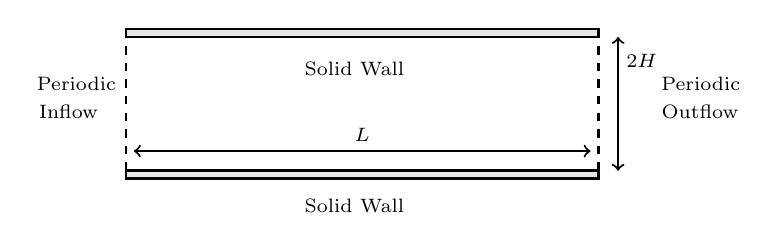
\begin{tikzpicture}
        % Draw a rectangle with specified properties
        \draw[line width=1pt, fill=gray!20] (0.0,1.8) rectangle (6.0,1.9);
        \draw[line width=1pt, fill=gray!20] (0.0,0.0) rectangle (6.0,0.1);
        \draw[dashed, line width=1pt] (0,0.1) -- (0,1.9);
        \draw[dashed, line width=1pt] (6,0.1) -- (6,1.9); 
        
        \node at (2.6+0.3, 1.4) {\scriptsize Solid Wall};
        \node at (2.6+0.3, -0.35) {\scriptsize Solid Wall};
    
        \node at (-0.63, 1.2) {\scriptsize Periodic};
        \node at (-0.73, 0.85) {\scriptsize Inflow};
    
        \node at (7.15+0.15, 1.2) {\scriptsize Periodic};
        \node at (7.15+0.14, 0.85) {\scriptsize Outflow};
    
        % draw arrows
        \draw[<->, line width=0.75pt] (0.1, 0.35) -- (5.9, 0.35);
        \node at (3.0, 0.55) {\scriptsize $L$};
    
        \draw[<->, line width=0.75pt] (6.25, 0.1) -- (6.25, 1.8);
        \node at (6.55, 1.5) {\scriptsize $2H$};
        
    \end{tikzpicture}
    \captionsetup{width=0.85\textwidth}
    \caption{Computational domain for the turbulent channel flow.}
    \label{fig: fully developed turbulent channel flow}
\end{figure}

The simulation is operated at Reynolds number \(\text{Re}_H = 22000\) based on the half-channel height \(H\). However, in turbulence modeling and especially for the turbulent channel flow, the Friction Reynolds number (\(\text{Re}_\tau \)) given by \(\text{Re}_\tau := (U_\tau H) / \nu \) is often used as a measure of the flow. The simulation is operated at \(\text{Re}_\tau = 550\). 

\begin{table}
    \centering
    \begin{tabular}{m{2.1cm} m{1.75cm} m{1.75cm} m{1.75cm} m{1.75cm}}
        \hline
        & $\mathbf{u}$ & $p$ & $k$ & $\varepsilon$ \\
        \hline
        \textbf{Inflow} & periodic & $p=p_{\text{in}}$ & periodic & periodic \\
        \textbf{Outflow} & periodic & $p=p_\text{out}$ & periodic & periodic \\
        \textbf{Solid walls} & $0$ & $\nabla p \cdot \mathbf{n} = 0$ & $0$ & $\nabla \varepsilon \cdot \mathbf{n} = 0$ \\
        \hline
    \end{tabular}
    \captionsetup{width=0.85\textwidth}
    \caption{Boundary conditions for the turbulent channel flow.}
    \label{tab: boundary conditions for the channel flow}
\end{table}

To verify the accuracy of the model, numerical results are compared to a direct numerical simulation performed by \cite{lee_direct_2015}. The same simulation is conducted for a series of meshes with varying values of \(d^+\), ranging from \(16\) to \(0.5\) (smaller value indicates finer mesh), with results provided in Figure \ref{fig: channel flow profiles} (for better clarity, results corresponding to some values of \(d^+\) are not shown). 

\begin{figure}[htbp]
    \centering
    \includegraphics[width=0.825\textwidth]{channel flow-profiles.pdf}
    \captionsetup{width=0.85\textwidth}
    \caption{Comparison of velocity (top) and turbulent kinetic energy (bottom) profiles obtained on meshes with different resolutions with direct numerical simulation (left), together with close-up plots (right).}
    \label{fig: channel flow profiles}
\end{figure}

We feel, considering the solution profiles from Figure \ref{fig: channel flow profiles}, and the fact that the fields are most sensitive in the viscous sub-layer that a value of \(d^+ = 2\) strikes a good balance between computational efficiency and numerical accuracy. For this mesh in particular, number of elements in the mesh is \(864\). Velocity and pressure spaces have \(3480\) and \(511\) degrees of freedom respectively. On the other hand, both \(k\) and \(\varepsilon\) function spaces have \(438\) degrees of freedom. Since results for mesh with value \(d^+ = 2\) and \(d^+ = 0.5\) do not differ dramatically, the former value will also be used when constructing a mesh for the next flow case.  

\subsection{Flow over a backward-facing step}

Flow over a backward-facing step occurs when a fluid flows over a sudden expansion, creating a separated flow region and a complex re-circulation zone downstream of the step. Domain and boundary conditions are constructed such that they match the data from the experiment performed by \cite{driver_features_1985}. Both can be seen in Figure \ref{fig: backward facing step} and Table \ref{tab: boundary conditions for the backward facing step} respectively. This is a significantly more complex scenario than the channel flow, making it a perfect validation case for the model. Because of the mesh size, a steady-state solver was used to obtain the result.    

\begin{figure}[htbp]
    \centering
    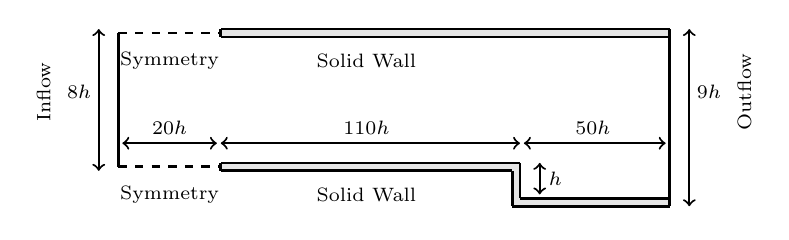
\begin{tikzpicture}
    
        \fill[gray!20] (2.3,1.7) rectangle (8.0,1.8);
        \draw[solid,  line width=1pt]     (2.3,1.7) -- (8.0,1.7);
        \draw[solid,  line width=1pt]     (8.0,1.7) -- (8.0,1.8);
        \draw[solid,  line width=1pt]     (8.0,1.8) -- (2.3,1.8);
        \draw[solid,  line width=1pt]     (2.3,1.8) -- (2.3,1.7);
        
        \fill[gray!20] (2.3,0.0) rectangle (6,0.1);
        \fill[gray!20] (6,-0.45) rectangle (8,-0.35);
        \fill[gray!20] (6,-0.45) rectangle (6.1,0.1);

        \draw[solid,  line width=1.0pt]     (2.3,0.0) -- (6.0,0.0);
        \draw[solid,  line width=1.0pt]     (6.0,0.0) -- (6.0, -0.45);
        \draw[solid,  line width=1.0pt]     (6.0, -0.45) -- (8.0, -0.45);
        \draw[solid,  line width=1.0pt]     (8.0, -0.45) -- (8.0, -0.35);
        \draw[solid,  line width=1.0pt]     (8.0, -0.35) -- (6.1, -0.35);
        \draw[solid,  line width=1.0pt]     (6.1, -0.35) -- (6.1, 0.1);
        \draw[solid,  line width=1.0pt]     (6.1, 0.1) -- (2.3, 0.1);
        \draw[solid,  line width=1.0pt]     (2.3, 0.1) -- (2.3, 0.0);
    
        \draw[dashed, line width=1pt]     (1.,1.75) -- (2.3,1.75);
        \draw[dashed, line width=1pt]     (1.,0.05) -- (2.3,0.05);
        \draw[solid,  line width=1pt]     (1.,0.05) -- (1.,1.75);
        \draw[solid,  line width=1pt]     (8,-0.35) -- (8,1.7);
    
        % Add text labels
        \node at (2.15+2.0, 1.4) {\scriptsize Solid Wall};
        \node at (2.15+2.0, -0.3) {\scriptsize Solid Wall};
    
        \node at (1.65, 1.4) {\scriptsize Symmetry};
        \node at (1.65, -0.3) {\scriptsize Symmetry};
    
        \node[rotate=90] at (0.05, 1.) {\scriptsize Inflow}; 
        \node[rotate=90] at (8.95, 1.) {\scriptsize Outflow};
    
        % draw arrows
        \draw[<->, line width=0.75pt] (6.35, 0.1) -- (6.35, -0.3);
        \node at (6.55, -0.1) {\scriptsize $h$};
    
        \draw[<->, line width=0.75pt] (1.05, 0.35) -- (2.25, 0.35);
        \node at (1.65, 0.55) {\scriptsize $20h$};
        
        \draw[<->, line width=0.75pt] (2.3, 0.35) -- (6.1, 0.35);
        \node at (4.15, 0.55) {\scriptsize $110h$};
        
        \draw[<->, line width=0.75pt] (6.15, 0.35) -- (7.95, 0.35);
        \node at (7.025, 0.55) {\scriptsize $50h$};
    
        \draw[<->, line width=0.75pt] (8.25, -0.45) -- (8.25, 1.8);
        \node at (8.5, 1.) {\scriptsize $9h$};
    
        \draw[<->, line width=0.75pt] (0.75, 0.0) -- (0.75, 1.8);
        \node at (0.5, 1.) {\scriptsize $8h$};
        
    \end{tikzpicture}
    \captionsetup{width=0.85\textwidth}
    \caption{Computational domain for the flow over backward-facing step.} 
    \label{fig: backward facing step}
\end{figure}

The Reynolds number based on the step height \(h\) is approximately \(\text{Re}_h = 36000\), where the reference velocity used to compute \(\text{Re}_h\) is measured just before encountering the step, specifically at \(x = -4h\) (with the step located at \(x=0\)). Computational mesh consists of \(129 844\) elements. There are \(523 038\) and \(65 838\) degrees of freedom for velocity and pressure spaces respectively, and \(65 838\) for both \(k\) and \(\varepsilon\) spaces. 

\begin{table}
    \centering
    \begin{tabular}{m{2.1cm} m{1.75cm} m{1.75cm} m{1.75cm} m{1.75cm}}
        \hline
        & $\mathbf{u}$ & $p$ & $k$ & $\varepsilon$ \\
        \hline
        \textbf{Inflow} & $\mathbf{u}_{\text{in}}$ & $\nabla p \cdot \mathbf{n} = 0$
        & $k_{\text{in}}$ & $\varepsilon_{\text{in}}$
        \\
        \textbf{Outflow} & $\nabla \mathbf{u} \cdot \mathbf{n} = 0$ & $p=0$ 
        & $\nabla k \cdot \mathbf{n} = 0$ & $\nabla \varepsilon\cdot \mathbf{n} = 0$
        \\
        \textbf{Solid walls} & $0$ & $\nabla p \cdot \mathbf{n} = 0$ 
        & $0$ & $\nabla \varepsilon \cdot \mathbf{n} = 0$
        \\
        \textbf{Symmetry} & $\mathbf{u} \cdot \mathbf{n} = 0$ & $\nabla p \cdot \mathbf{n} = 0$ 
         & $\nabla k \cdot \mathbf{n} = 0$ & $\nabla \varepsilon \cdot \mathbf{n} = 0$
        \\
        \hline
    \end{tabular}
    \captionsetup{width=0.85\textwidth}
    \caption{Boundary conditions for the flow over backward-facing step.}
    \label{tab: boundary conditions for the backward facing step}
\end{table}

The model's accuracy is verified using experimental data from \cite{driver_features_1985}. A key measure of success is accurately predicting the reattachment point downstream of the step. This is determined by measuring the point \(\hat{x}\) where the skin friction coefficient (\(C_f\)) is equal zero. In the experiment, this was done using a laser oil-flow interferometer. Another measure for analyzing the results is the pressure coefficient (\(C_p\)). The results in Figure \ref{fig: backstep coefficients} show a poor match between the simulation and experiment, with the reattachment point observed at \(\hat{x} = 6.26 h\) compared to the simulation's \(\hat{x} = 5.0 h\). However, this discrepancy is expected from the \(k\)-\(\varepsilon\) model, which is known to struggle with separation and adverse pressure gradients. When compared to results in article by \cite{steffen_jr._critical_1993} with multiple versions of \(k\)-\(\varepsilon\) model, with reattachment points ranging from \(\hat{x} = 4.9\) to \(\hat{x} = 5.5\), we see a better match.

\begin{figure}[htbp]
    \centering
    \includegraphics[width=0.825\textwidth]{backstep-coefficients.pdf}
    \captionsetup{width=0.85\textwidth}
    \caption{Comparison of the skin-friction coefficient (left) and the pressure coefficient (right) between experiment and simulation.}
    \label{fig: backstep coefficients}
\end{figure}

Figure \ref{fig: backstep profiles} presents normalized velocity magnitude \(U/U_\infty\) and \(k\) profiles at four points after the step. While the velocity profiles show good agreement, \(k\) diverges after \(x = 4h\), which is likely the cause of the reattachment point appearing prematurely. 

\begin{figure}[htbp]
    \centering
    \includegraphics[width=0.825\textwidth]{backstep-profiles.pdf}
    \captionsetup{width=0.85\textwidth}
    \caption{Comparison of velocity (top) and turbulent kinetic energy (bottom) profiles at \(x = 1h\) (left), \(x = 4h\) (second left), \(x = 6h\) (second right) and \(x = 10h\) (right) between experiment and simulation.}
    \label{fig: backstep profiles}
\end{figure}

% Section 4 - Conclusion
\section{Conclusion}

The Lam--Bremhorst \(k\)-\(\varepsilon\) turbulence model was implemented successfully in FEniCS computing platform, both in the transient and steady-state formulation. We verified the implementation of the transient solver by simulating a fully developed channel flow, where a very good agreement was found between the computed solutions and the DNS. While the results of the backward-facing step simulation did not match the experiment, we still consider the implementation of the steady-state solver a success, as the results matched the expected behavior of the \(k\)-\(\varepsilon\) model. It is clear from those results that implementing the working \(k\)-\(\varepsilon\) model in FEniCS can be done with relative ease, and we do not see any reason why that would not be true for different turbulence models such as the \(k\)-\(\omega\) or the Spalart-Allmaras. These results can be replicated via scripts archived at \href{https://github.com/joove123/k-epsilon}{https://github.com/joove123/k-epsilon}.

\begin{acknowledgement}
    I would like to thank my master's thesis supervisor, Prof. Achim Schroll, for his professional guidance and support during the writing of my master's thesis and this article. I also thank NumFOCUS for the travel award that enabled me to attend the FEniCS 2024 conference. 
\end{acknowledgement}

% ---- Article ends here ---- 

\bibliographystyle{spbasic}

% Write the full path of your bibfile relative to book.tex
\bibliography{chapters/marcibal/bibliography.bib}

\graphicspath{{chapters/chp1/graphics/}}


\title{Growth and Remodelling Package in FEniCSx}

\author{Karl Munthe, Henrik Finsberg, Samuel Wall, Joakim Sundnes}

\institute{K. Munthe \at Simula Research Laboratory, Oslo, Norway and \\ Department of Informatics, University of Oslo, Norway, \email{karlfredrik@simula.no}
\and
H. Finsberg \at Simula Research Laboratory, Oslo, Norway
\and
S. Wall \at Simula Research Laboratory, Oslo, Norway
\and
J. Sundnes \at Simula Research Laboratory, Oslo, Norway and \\ Department of Informatics, University of Oslo, Norway}

\maketitle
\abstract{The heart is a dynamic organ that changes its size and shape to regulate its behaviour to the demands of the body, which can change for example through body growth, exercise, the onset of a disease, or taking medication. Different models exist to try to capture various types of cardiac growth as a result of mechanical stimuli. In this manuscript we will present a framework created with FEniCSx that allows one to quickly run simulations of growth and remodelling with different material models and different growth laws. We present some of the simulations and compare them to the relevant literature in the field. \added{All the code can be found at \url{https://github.com/karlfm/Growth-and-Remodeling-in-FEniCSx}}}
\vspace{12pt}
\section{Introduction}
In classical continuum mechanics one normally studies the mechanics of bodies where mass\replaced{, linear momentum, angular momentum, and energy are conserved properties}{is a conserved property conserved property}. This approach has been extremely successful and is the bedrock for traditional engineering disciplines, but it does not accurately capture aspects of how living organisms change with respect to their environment. One of the unique features of biological material is its ability to grow and evolve by adding or removing mass. Understanding how biological matter grows and what drives the growth is important, not only to understand normal growth and development, but also when and how growth may become non-compensatory and drive disease.\par It has been known for a long time that the growth of organs, such as the heart, is regulated at least in part by the forces applied to it \citep{Hsu1968}. This understanding has led to the formulation of growth laws that link growth and remodeling to local stress or strain. \par
In this chapter we will introduce a package written in FEniCSx that allows one to easily model growth and remodelling of biological tissue, with the aim of quickly testing combinations of growth models and material models. Allowing researchers to systematically test combinations of material models and growth tensors will aid in the discovery of more accurate models of growth and remodelling phenomena of biological tissue.
\section{Methods}
\subsection{Growth and Remodeling in Continuum Mechanics}
Consider a solid body that is continuously and smoothly deforming from one configuration to another, and denote the initial configuration (also called the reference configuration) as $\mathcal{M}$ and the current configuration $\mathcal{N}$. We denote a point in $\mathcal{M}$ with uppercase letters $\mathbf{X} = (X, Y, Z)$ and a point in $\mathcal{N}$ with lowercase letters $\mathbf{x} = (x, y, z)$\footnote{Apart from the letters $X$, $Y$, and $Z$, all upper case letters represent tensors.}. A point in $\mathcal{M}$ can be mapped to a point in $\mathcal{N}$ by a motion, $\phi(\mathbf{X}): \mathbf{X} \rightarrow \mathbf{x}$, which is a diffeomorphism. We can map a vector from the reference configuration to the current configuration via the pushforward of $\phi$, which is commonly denoted by $\mathbf{F}$ and is referred to as the deformation gradient, computed as $\mathbf{F} = \partial\mathbf{x}/\partial\mathbf{X}$. The displacement field $\mathbf{u} = \mathbf{x} - \mathbf{X}$ is a vector field describing the displacement of each point $\mathbf{X}$ in the reference configuration to its location $\mathbf{x}$ in the deformed configuration. \par 
Most mechanical models of the heart assume that the tissue is hyperelastic, meaning that deformations of the material conserve its energy, and when any load on the tissue is removed it returns to its original reference shape. Growth, on the other hand, represents a permanent change of the unloaded reference configuration, and cannot be modeled as an elastic deformation. Instead, it is commonly modeled using the framework of plastic or elasto-plastic deformations. The most common framework is to multiplicatively split the deformation tensor into an elastic part and a growth part, 
\begin{equation}
\label{eq: multiplicative split}
    \mathbf{F} = \mathbf{F}_e\mathbf{F}_g,
\end{equation}
where $\mathbf{F}_e$ is the elastic deformation and $\mathbf{F}_g$ is the plastic deformation that represents growth. Among the early adopters of the multiplicative split of elastic and plastic deformations in biological tissue were by \citep{Kondaurov1987}, \citep{Takamizawa1990}, and \citep{Rodriguez1994}. \par 
\added{One interpretation of \ref{eq: multiplicative split} is that the material first deforms by $\mathbf{F}_g$ in a way that does not cause stress, but might cause incompatibilities in the form of discontinuities or overlapping material. The deformation described by $\mathbf{F}_g$ leads to an unphysical intermediate configuration, which is then deformed by $\mathbf{F}_e$} \deleted{Then it deforms by $\mathbf{F}_e$}in a way that removes the unphysical characteristics that occurred from $\mathbf{F}_g$, but adds residual stress. \added{Sufficient conditions for the existence of intermediate configurations such as $\mathbf{F}_g$ are discussed in \citep{Goodbrake2021}}. We assume that the deformation described by $\mathbf{F}_e$ is hyperelastic, such that we can obtain the first Piola–Kirchhoff stress tensor by differentiating a strain energy function,
\begin{equation}
\label{eq: stress}
    \mathbf{P} = \frac{\partial\Psi}{\partial \mathbf{F}_e}.
\end{equation}
The total deformation due to growth is obtained by 
\begin{equation*}
    \mathbf{F}_g^{i + 1} = \mathbf{F}_g^i\mathbf{F}_g^\mathrm{inc},
\end{equation*}
where $\mathbf{F}_g^\mathrm{inc}$ is the incremental growth tensor, and $\mathbf{F}_g^i$ is the cumulative growth that has occurred after $i$ steps. The initial growth tensor, $\mathbf{F}_g^0$, is set to the identity tensor. The reason we have to use this form of the growth tensor is because we are always mapping from the same reference configuration; so after $n$ steps, we are applying $n$ growth deformations, which looks like 
\begin{equation*}
    \mathbf{F}_g^{n} = \mathbf{F}_{g}^\mathrm{inc}\vert_{t=0}\mathbf{F}_{g}^\mathrm{inc}\vert_{t=1} \cdots \mathbf{F}_{g}^\mathrm{inc}\vert_{t=n},
\end{equation*}  
where $\mathbf{F}_{g}^\mathrm{inc}\vert_{t=i}$ means the $\mathbf{F}_{g}^\mathrm{inc}$ at the $i$'th step. Note that the $i$'th incremental growth tensor is dependent on the stress or strain that occurred in the $i-1$'th growth step (see \citep{Goriely2007}). It is common to express the incremental growth tensor in terms of fiber, crossfiber, and normal directions 
\begin{equation*}
    \mathbf{F}_g^\mathrm{inc} = F^\mathrm{inc}_{g,f}\mathbf{e}_f\otimes \mathbf{e}_f + F^\mathrm{inc}_{g,c}\mathbf{e}_c\otimes \mathbf{e}_c + F^\mathrm{inc}_{g,n}\mathbf{e}_n\otimes \mathbf{e}_n.
\end{equation*}
where $F^\mathrm{inc}_{g, i}$ for  $i = \{f, c, n\}$ are functions of either stress or strain, and $\mathbf{e}_i$ for $i = {\{f, c, n\}}$ are orthonormal basis vectors in the fiber, crossfiber, and normal directions respectively. The equations are then furnished with boundary conditions that that describe the load and displacement of the boundary,
\begin{equation} \label{eq: system of equations}
\begin{aligned}
    \mathbf{F} & = \mathbf{F}_e\mathbf{F}_g && \text{in } \mathcal{M} ,\\
    \nabla\cdot\mathbf{P} & = 0 && \text{in } \mathcal{M}, \\
    \mathbf{P}\cdot \nu & = 0 && \text{on } \partial\mathcal{M}_N, \\
    \mathbf{u} & = g_D && \text{on } \partial\mathcal{M}_D,
\end{aligned}
\end{equation} 
where $\nu$ is a surface normal vector, $\partial\mathcal{M}_N$ amd $\partial\mathcal{M}_D$ denote the boundaries which are prescribed Neumann and Dirichlet boundary conditions respectively. Finally, we need to specify the material model, and in this paper we use a \replaced{nearly}{weakly} incompressible neo-Hookean model, so (\ref{eq: stress}) becomes
\begin{align*}
    \mathbf{P} &= \frac{\partial\Psi_\text{iso}}{\partial \mathbf{F}_e} + \frac{\partial\Psi_\text{vol}}{\partial \mathbf{F}_e}, \\
    \mathbf{P} &= \frac{\partial}{\partial \mathbf{F}_e}\left[\frac{\mu}{2}\left(\tr\mathbf{\bar{C}} - 3\right) + \kappa(J-1)^2\right],
\end{align*}
where and $\mu$ and $\kappa$ material parameters. $\Psi_\text{iso}$ and $\Psi_\text{vol}$ are the isochoric (distortional) and volumetric (dilational) parts of the strain energy function. To decouple the energy stored in the body as a result of volume preserving deformation and non-volume preserving deformation, we set $\mathbf{\bar{F}}_e = \mathbf{F}_eJ^{-1/3}$, whose determinant is equal to the identity tensor. The isochoric right Cauchy-Green deformation tensor, $\mathbf{\bar{C}}$, is calculated as $\mathbf{\bar{C}} = \mathbf{\bar{F}}_e^\top \mathbf{\bar{F}}_e$. Now, $\partial\Psi_\text{iso}/\partial \mathbf{F}_e = 0$ only if the deformation preserves the shape, and $\partial\Psi_\text{vol}/\partial \mathbf{F}_e = 0$ only if the deformation preserves the volume (see chapter 6 of \citep{Holzapfel2002} for more details). \par 
For further information about continuum mechanics we recommend \citep{Marsden1983} and \citep{Holzapfel2002}, and for further information about growth and remodelling we recommend \citep{Goriely2017} and \citep{Yavari2010}.

\subsection{Numerical Implementation And Experiments}
 
\added{Algorithm \ref{alg:growth_deform} shows the algorithm used for strain based growth. For stress based growth, you would update the stress tensor rather than the strain tensor, and for additive growth laws, you would add the cumulative and incremental growth tensors instead of multiplying them together.} \par
\begin{algorithm} 
    \caption{Growth tensor and stress/strain tensor are updated at each growth step. Both $\mathbf{F}_\mathrm{e}$ and $\mathbf{F}_g^\mathrm{inc}$ are dependent on $\mathbf{u}$.}\label{alg:growth_deform}
    \SetAlgoLined
    \For{each time step}{
        Solve (\ref{eq: system of equations}) for the displacement $\mathbf{u}$\;
        Update the stress/strain tensor using $\mathbf{u}$ from the previous line.\;
        Update the growth tensor using the stress/strain tensor from the previous line.\;
    }
\end{algorithm} 
\emph{Constructing the weak form}: We multiply $\nabla\cdot\mathbf{P}$ by a test function, which we set to be in the same function space as $\mathbf{u}$, and integrate over a discretization of $\mathcal{M}$. By applying integration by parts, we obtain
\begin{align}
    \label{eq: weak conservation of momentum}
    \int_\Omega(\nabla\cdot\mathbf{P})\cdot\eta d\mathbf{X} &= 0  \notag\\
    \int_\Omega \mathbf{P} : \nabla\eta d\mathbf{X} &= \int_{\partial\Omega}\mathbf{P}\cdot\eta \cdot \nu dA.
\end{align}
\replaced{Since we are using test functions, $\eta$, that vanish on $\partial_D\mathcal{M}$, and the normal component of $\mathbf{P}$ is zero on $\partial_N\mathcal{M}$ we can set the boundary integral to zero. }{Since we are using Dirichlet boundary conditions, $\mathbf{P} = 0$ on the boundary of $\mathcal{N}$}. (\ref{eq: weak conservation of momentum}) is solved using FEniCSx \cite{DOLFINx}. 
\par
\emph{Iteratively solving the conservation of momentum}: We now solve (\ref{eq: weak conservation of momentum}) for the displacement $\mathbf{u}$, which we can use to compute all the necessary variables. \added{We use tetrahedral, second order, continuous, Lagrange elements to approximate $\mathbf{u}$; and a first order, discontinuous, Lagrange elements to approximate $\mathbf{F}_e$ and $\mathbf{F}_g$. This is a common numerical scheme in cardiac mechanics which has been demonstrated to avoid locking \citep{oliveira2016comparison}.} $\mathbf{F}_g$ is initially set to be the identity tensor. \par
\subsection{Solving Growth Laws on the Unit Cube}
\label{subsec: simulations}
In the simulations we have run we have aligned the $x$-axis with the fiber direction and the $y$-, and $z$-axis are the crossfiber and normal direction. To be consistent with the literature we will use $\mathbf{e}_f$, $\mathbf{e}_c$, and $\mathbf{e}_n$ to denote the unit vectors in the $(x, y, z)$ directions respectively.  \par
\emph{Boundary conditions:} We set the following boundary conditions
\begin{align*}
    g_D = \begin{cases}
        u &= \begin{cases}
            0 & \text{on } x = 0, \\
            u_D & \text{on } x = 1,
        \end{cases} \\
        v &= 0 \qquad \ \ \text{on } y = 0, \\
        w &= 0 \qquad \ \ \text{on } z = 0,
    \end{cases}
\end{align*}
where $u$, $v$, and $w$ are the displacement in the $x$, $y$, and $z$ direction respectively. $u_D$ specifies how much the body is displaced. 
\par

\emph{Numerical simulations:} We ran two simulations, one with a 10\% stretch and one with a 10\% compression which corresponds to $u_D = 0.1$ and $u_D = -0.1$ respectively. For the GCG model, $F_{g,c,\mathrm{max}}$ was set to 1.2 in the stretch simulation and 0.8 in the compression simulation (see table \ref{tab:growth models}). We set $\mu = 15$ kPa and $\kappa = 100$ kPa.
\subsection{The different growth models}
\label{sub:different models} 
In this paper we compare five growth models which we have taken from \citep{Taber1998}, \citep{Kroon2009}, \citep{Goktepe}, and \citep{Kerckhoffs2012}. The growth models are given in table \ref{tab:growth models} where LT2 is from \citep{Taber1998}, KFR is from \citep{Kroon2009}, GEG and GCG are from \citep{Goktepe} and KOM is from \citep{Kerckhoffs2012}. Each growth model had a set point that either determined the homeostatic level of stress, stretch, or strain. When the stress, stretch, or strain reaches the set point, then growth will cease to occur. If this does not happen, the body will grow indefinitely, which we call runaway growth. We used the same variables as they were given in the original papers, except for the \replaced{GCG}{$GCG$}, where we scaled the variables to more accurately fit with the shear modulus used here. The values are tabulated in table \ref{tab:parameters}.
%\newgeometry{right=1cm, left=1cm}%,right=1cm,top=1cm,bottom=1cm}
\begin{table}
\centering
\makebox[\textwidth][c]{
\renewcommand{\arraystretch}{4}
\begin{tabular}{|c||c|c|c|}
\hline \hline
 & $F_{g,f}^{i+1}$ & $F_{g,n}^{i+1}$ & $F_{g,c}^{i+1}$ \\
\hline \hline
LT2 & $\displaystyle F_{g,f}^i\left(\frac{\sigma_{\theta p} - \sigma_{p,0}}{T\sigma_{p,0}} + 1\right)$ & $\displaystyle F_{g,n}^i\left(\frac{\sigma_{\theta a} - \sigma_{a,0}}{T\sigma_{a,0}} + 1\right)$ & $\displaystyle 1$ \\
\hline
KFR & $\displaystyle F_{g,f}^i(\beta(\sqrt{2 E_{ff} + 1} - 1 - s_\mathrm{hom}) + 1)^{1/3}$ & $\displaystyle F_{g,n}^i(\beta(\sqrt{2 E_{ff} + 1} - 1 - s_\mathrm{hom}) + 1)^{1/3}$ & $\displaystyle F_{g,c}^i(\beta(\sqrt{2 E_{ff} + 1} - 1 - s_\mathrm{hom}) + 1)^{1/3}$ \\
\hline
GEG & $\displaystyle \frac{1}{\tau}\left(\frac{F_{g,f,\mathrm{max}} - F_{g,f}^i}{F_{g,f,\mathrm{max}} - 1}\right)^\gamma(F_{e, f}^i - \lambda^\text{crit}) + F^i_{g, f}$ & $\displaystyle 1$ & $\displaystyle 1$ \\
\hline
GCG & $\displaystyle 1$ & $\displaystyle  \frac{1}{\tau}\left(\frac{F_{g,c,\mathrm{max}} - F_{g,c}^i}{F_{g,c,\mathrm{max}} - 1}\right)^\gamma(\tr(\mathbf{M}) - p^\mathrm{crit}) + F^i_{g, c}$ & $\displaystyle 1$ \\
\hline
KOM & $\displaystyle \begin{cases}
        F_{g,f}^{i}k_{ff}\frac{f_\mathrm{ff, max}\Delta t_\text{growth}}{1 + \exp(-f_f(s_\mathrm{l}-s_{l,50}))} + 1, \qquad s_\mathrm{l} \geq 0\\
        F_{g,f}^{i}\frac{-f_\mathrm{ff, max}\Delta t_\text{growth}}{1 + \exp(f_f(s_\mathrm{l}+s_{l,50}))} + 1, \qquad s_\mathrm{l} < 0
    \end{cases} $ & $\displaystyle \begin{cases}
        F_{g,c}^{i}\sqrt{k_{cc}\frac{f_{cc,\mathrm{max}}\Delta t_\text{growth}}{1 + \exp(-c_\mathrm{f}(s_\mathrm{t}-s_{t,50}))} + 1}, \qquad s_\mathrm{t} \geq 0\\
        F_{g,c}^{i}\sqrt{\frac{-f_{cc,\mathrm{max}}\Delta t_\text{growth}}{1 + \exp(c_\mathrm{f}(s_\mathrm{t}+s_{t,50}))} + 1}, \qquad s_\mathrm{t} < 0 
    \end{cases} $ & $\displaystyle \begin{cases}
        F_{g,c}^{i}\sqrt{k_{cc}\frac{f_{cc,\mathrm{max}}\Delta t_\text{growth}}{1 + \exp(-c_\mathrm{f}(s_\mathrm{t}-s_{t,50}))} + 1}, \qquad s_\mathrm{t} \geq 0\\
        F_{g,c}^{i}\sqrt{\frac{-f_{cc,\mathrm{max}}\Delta t_\text{growth}}{1 + \exp(c_\mathrm{f}(s_\mathrm{t}+s_{t,50}))} + 1}, \qquad s_\mathrm{t} < 0 
    \end{cases} $ \\
\hline
\end{tabular}
}
\caption{$F_{g,f}$, $F_{g,c}$, $F_{g,n}$,  for each of the five models. The parameters $T$, $\beta$, $\tau$, and $\Delta t$, simply determine the rate of growth and can be tuned to \replaced{match}{math} the growth rate of data obtained from experiments.}
\label{tab:growth models}
\end{table}
%\restoregeometry
\begin{table}[htbp]
    \centering
    \begin{tabular}{|l|l|}
    \hline
    \textbf{Model} & \textbf{Parameters} \\
    \hline
    \textbf{LT2} &   $\sigma_{a,0} = 30$ [kPa], $\sigma_{p,0} = 3$ [kPa], $T = 10^{-4}$ \\ \hline
    \textbf{KFR} &  $s_\mathrm{hom} = 0.13, \beta = 10^{-2}$ \\ \hline
    \textbf{GEG} &  $F_{g,f,\mathrm{max}}=1.5$, $\lambda^\mathrm{crit}=1.01$, $\gamma = 2$, $\tau = 10^2$ \\ \hline
    \textbf{GCG} &  $F_{g,c,\mathrm{max}}=1.2$ and $0.8$,  $p^\mathrm{crit}=0.12, \gamma = 2, \tau = 10^4$ \\ \hline
    \textbf{KOM} &  $f_\mathrm{ff,max} =0.31$ [1/days], $f_f = 150$, $s_{l50} = 0.06$, $F_{ff50} = 1.35$, $f_{l,\mathrm{slope}} = 40$, $f_\mathrm{ff,max} = 0.1$ [1/days] \\
        & $c_\mathrm{f} = 75$, $s_\mathrm{t50} = 0.07$, $F_\mathrm{cc50} = 1.28$, $c_\mathrm{th,slope} = 60$, $E_{ff,\mathrm{set}} = 0$, 
        $E_\mathrm{cross,\mathrm{set}} = 0$, $\Delta t = 10^{-2}$ [days] \\ \hline
    \end{tabular}
    \caption{Model parameters for the growth models. $T$, $\beta$, $\tau$, and $\Delta t$, determine the speed of growth.}
    \label{tab:parameters}
\end{table}
In LT2, $\sigma_{p,0}$ and $\sigma_{a,0}$ are set points for the passive and active fiber stress at equilibrium, and $\sigma_{\theta p}$ and $\sigma_{\theta a}$ are the active and passive fiber stresses. In the simulations we have run, we have only used the passive component of $\sigma$, and have set $\sigma_a = 0$. For KFR, $s_\mathrm{hom}$ is the strain set point. For GEG and GCG, $F_{g,f,\mathrm{max}}$ and $F_{g,c,\mathrm{max}}$ is the maximum amount of growth allowed to occur. $\mathbf{M}$ is the Mandel stress, which is defined as 
\begin{equation*}
    \mathbf{M} = \mathbf{F}^\top \mathbf{P}
\end{equation*}
and $p^\mathrm{crit}$ is the stress set point. $\lambda^\text{crit}$ is the strain set point. For KOM, $k_{ff}$ and $k_{cc}$ are defined as
\begin{align*}
    k_{ff} &= \frac{1}{1 + \exp(f_\text{length,slope}(\mathbf{F}_{g,ff}^i - F_{ff,50}))} \\
    k_{cc} &= \frac{1}{1 + \exp(c_\text{thickness,slope}(\mathbf{F}_{g,cc}^i - F_{cc,50}))}
\end{align*}
and $s_\mathrm{l}$, and $s_\mathrm{t}$ are defined as
\begin{align*}
    s_\mathrm{l} &= \max(E_{ff}) - E_{ff, \mathrm{set}} \\
    s_\mathrm{t} &= \min(E_\text{cross, max}) - E_\mathrm{cross, set}
\end{align*}
where $E_{ij}$ is the Lagrange strain tensor, and $E_{ff}$ is the strain in the fiber direction, and $E_\text{cross, max}$ is the maximum algebraic maximum principle strain of the matrix (see \citep{Witzenburg2018})
\begin{equation*}
    E_\text{cross} = \begin{pmatrix}
        E_{cc} & E_{cr} \\
        E_{rc} & E_{rr}
    \end{pmatrix}
\end{equation*}
and $E_{ff, \mathrm{set}}$ and $E_\mathrm{cross, set}$ are set points. \par
\deleted{In the simulations run, LT2 displayed runaway growth as was also observed in the simulations run in }\citep{Witzenburg2018}. Growth stops for the LT2 model when $\sigma_{\theta} = \sigma_{0}$.
\deleted{which was not satisfied in our simulations or in the simulations run by} \citep{Witzenburg2018}. For KOM, since $k_{cc}$ and $k_{ff}$ are logistic functions, the growth is bounded from above and below inhibiting runaway growth. Finally, for KFR, it does not appear obvious that it will not obtain runaway growth, but other simulations setups that were tested did result in runaway growth, even though the one we present here does not.
\section{Results}
The data we collected from the two simulations (see section \ref{subsec: simulations}) were the the stretch and growth that occurred in the middle of the cube. The results are depicted in figures \ref{fig:10p_stretch} and \ref{fig:10p_compression}. The top row of each figure displays the fiber and crossfiber components of the growth tensor, $\mathbf{F}_g$, and the bottom row displays the fiber and crossfiber components of the elastic deformation tensor $\mathbf{F}_e$. In the simulations we ran, $\mathbf{F}_e$ is diagonal, so the components of $\mathbf{F}_e$ are the principle stretches. This is because $\sqrt{\mathbf{e}_i^\top\mathbf{C}_e\mathbf{e}_i}$ is the principle stretch in the $i$'th direction, and $\sqrt{\mathbf{e}_i^\top\mathbf{C}_e\mathbf{e}_i} = \sqrt{\mathbf{e}_i^\top\mathbf{F}_e^\top\mathbf{F}_e\mathbf{e}_i} = \mathbf{F}_e\mathbf{e}_i$. By the same reasoning, the diagonal components of $\mathbf{F}_g$ (which are the only non-zero components), give the growth in fiber, crossfiber, and normal direction. Increasing $\kappa$ did not yield qualitatively different results. \par
GCG seems to be converging to $F_{g,c,\mathrm{max}}$, and GEG seem to have converged because it reached $\lambda^\text{crit}$. The reason GCG is growing oppositely compared to GEG is probably because GEG was created to model growth triggered by volume overload while GCG was created to capture growth triggered by pressure overload. KFR grew an equal amount in each direction, and stabilized. It is not clear under what conditions KFR should be stable because $s_\mathrm{hom}$ is the same in each direction. When we ran simulations with other boundary conditions, the solution diverged. The KOM model was stable for many different types of boundary conditions, but is the most computationally expensive model to run.\par 
\begin{figure}[h]
    \centering
    \includegraphics[width=\textwidth]{10p_stretch_3.png}
    \caption{Growth and stretch predicted by a 10\% stretch in the fiber direction.}
    \label{fig:10p_stretch}
\end{figure}
\begin{figure}[h]
    \centering
    \includegraphics[width=\textwidth]{10p_compression_3.png}
    \caption{Growth and stretch predicted by a 10\% compression in the fiber direction.}
    \label{fig:10p_compression}
\end{figure}    
\section{Conclusion and future work}
We have implemented a general growth and remodelling framework using the FEniCSx program in Python. The goal is to easily change material models and growth models. This will allow researchers to compare their models with other models in the field. Future work will include implementing more complex geometries, more growth laws, and more material models. \added{The models we have used in this paper are not derived from the dissipation equation but are instead phenomenologically derived growth laws and future work should investigate whether or not they satisfy the laws of thermodynamics. Another avenue of future research we wish to pursue is to look into constrained mixture models which model how changes in the various constituents influence the characteristics of the tissue.} \deleted{Specifically, w}\added{W}e also wish to add models that have more mathematically sophisticated stopping criteria, such as the ones developed by Erlich et al. \citep{Erlich2023} uses an energy penalty to construct a stopping criteria and \citep{Erlich2024} looks into how curvature\footnote{The intrinsic three dimensional curvature, not the two dimensional curvature of the surface of the body.} in the reference configuration could be used as a stopping criteria. Future work will also implement the growth models on geometries with fibers. We tried running the models on various fiber orientations and found them extremely sensitive to fibers that varied throughout the domain. Preliminary results indicate that some of the models do not converge to a steady state for relatively small perturbations of the variables or if the fibers are not well aligned with the body, something we plan on quantifying in the future. \par
When this package is further developed we aim to add it to the Pulse\footnote{https://github.com/finsberg/fenicsx-pulse} package. \par
The models we compared have been developed to capture different aspects of growth and were tuned to be used on different material models, so an apples-to-apples comparison might not be fair. Furthermore, the growth models we have used are not taking into account residual stresses that exist within the material before or after growth occurs. \par
Finally, experimental data is needed to verify which models are accurate or capture the correct phenomena of growing cardiac tissue.
% \newpage
\bibliographystyle{spbasic}
\bibliography{chapters/chp1/bibliography.bib}
% \printbibliography
% \end{document}



% Write the full path to the location of the graphics relative to book.tex
\graphicspath{{chapters/chp1/graphics/}}

\title{Blood flow in the beating heart: Coupling fluid dynamics to reduced wall and circulation models for data-driven cardiac FSI}
\titlerunning{Blood flow in the beating heart}

\author{Marc Hirschvogel, Mia Bonini, Maximilian Balmus, David Nordsletten}
\authorrunning{Hirschvogel et al.}

\institute{Marc Hirschvogel \email{marc.hirschvogel@polimi.it} \at MOX, Dipartimento di Matematica, Politecnico di Milano, Milan, Italy}

\maketitle

\abstract{We present a fluid-reduced-solid interaction (FrSI) approach suitable for modeling blood flow in the beating left heart. 
The method uses image-derived model data to construct a suitable boundary motion space, enhanced by a reduced solid mechanics wall model to enable adaptive fluid motion. 
The method combines the efficiency of fluid dynamics models with features from full FSI approaches, uniquely integrating motion data to predict cardiac hemodynamics over a full heart cycle. 
The approach is presented for a patient-specific left heart model coupled to a lumped circulatory system, showing physiological flow behavior and pressure-volume relations.}


\section*{Introduction}
Computational fluid dynamics (CFD) provides a valuable tool to predict blood flow in the cardiovascular system \cite{schwarz2023}. 
Models of blood flow in the heart have become relevant to predict various cardiovascular conditions, where motion states from imaging are used \cite{bonini2022-suppl,zingaro2023,garciavillalba2021} or even fully-coupled fluid-solid interaction (FSI) models are employed \cite{nordsletten2011-fsi,mccormick2011modelling}. 
However, prescribed cavity motion reduces the model's ability to adapt under varying loads, and full FSI models are complex, computationally demanding, and difficult to constrain (uncertain boundary conditions and sparse patient data for reliable geometry reconstruction).
The fluid-reduced-solid interaction (FrSI) method closes the gap between model complexity and efficiency. This is a data-informed model reduction approach, particularly suited for cardiac FSI \cite{hirschvogel2024-frsi}. 
The method combines physics- with projection-based model reduction techniques that leverage Proper Orthogonal Decomposition (POD) modes derived from imaging (or some high-fidelity model) to build a reduced-order model (ROM), combined with a structural model of the ventricular wall defined on a 2D manifold.
In this contribution, we show the FrSI method's applicability to a complex, patient-specific left heart model, with a particular focus on monolithic solver implementations in FEniCSx \cite{alnaes2015fenics, baratta2023dolfinx}. This method encompasses the implementation of an Arbitrary Lagrangian-Eulerian (ALE) fluid mechanics problem subject to non-local constraints (Galerkin ROM, 3D-0D coupling to lumped circulation models). 
The solver and preconditioning aspects of this model and other fluid dynamics problems under non-local boundary conditions have been introduced in \cite{hirschvogel2025-prec}.


\section*{Methods}
The fluid-reduced-solid interaction (FrSI) problem of a 3D left heart model (atrium, ventricle, aortic outflow tract) along with the underlying data sources is depicted in Fig.~\ref{fig:heart_problem}. 
In particular, domain and motion data are retrieved from time-resolved dynamic computed tomography (CT), which are subsequently mapped to a finite element mesh in order to generate a discrete space of modes using POD \cite{rathinam2003}. 
The model is further coupled to a closed-loop systemic, pulmonary, and coronary circulation system \cite{hirschvogel2017,arthurs2016} in order to provide physiologically meaningful cardiovascular loads to the 3D model.
\begin{figure}[!htp]
\centering
\includegraphics[width=1\textwidth]{heart_problem}
\caption{\textbf{A.} Dynamic cardiac computed tomography (CT) images with contrast and dynamic segmentation of left heart lumen for subsequent finite element mesh generation, motion tracking of deformation over the heart cycle. 
\textbf{B.} Principal component analysis by means of Proper Orthogonal Decomposition (POD) of wall motion space. The first three most dominant POD modes are shown (10 are used). 
\textbf{C.} Partition of unity fields for regional decomposition of POD space: Atrium, ventricle, and aortic outflow tract---as well as their junctions and truncations around the in-/outflows---can exhibit independent kinematics. 
\textbf{D.} 3D-0D coupled FrSI model of the left heart.}\label{fig:heart_problem}
\end{figure}

\subsection*{Preprocessing of patient data}
The FrSI approach relies on external data sourced either from some high-dimensional model or from patient-specific imaging data. Here, we build a patient-specific model of the left heart by segmenting a dynamic cardiac CT data set using 3D Slicer \cite{kikinis2014-3dslicer}, cf. Fig.~\ref{fig:heart_problem}A. Subsequently, a diastolic frame is meshed with SimModeler \cite{simmodeler}, and a motion tracking algorithm is used to extract the wall velocities at each frame and map them to the finite element mesh (with velocity degree of freedom space of size $n_{v}$). Thereafter, the wall velocity data for $m=19$ frames is collected into a snapshot matrix $\hat{\boldsymbol{\mathsf{S}}} \in \mathbb{R}^{n_{v} \times m}$, and the eigenvalue problem
\begin{align}
    (\hat{\boldsymbol{\mathsf{S}}}^{\mathrm{T}} \hat{\boldsymbol{\mathsf{S}}}) \,\boldsymbol{\uppsi}_{i} = \uplambda_{i} \,\boldsymbol{\uppsi}_{i}, \quad i = 1, \hdots, m,\label{eq:rom_eigensolve}
\end{align}
is solved, with eigenvalues $\uplambda$ and eigenvectors $\boldsymbol{\uppsi} \in \mathbb{R}^{m}$. The first $r_{v}$ POD modes $\boldsymbol{\upphi} \in \mathbb{R}^{n_{v}}$ then can be computed as follows:
\begin{align}
    \boldsymbol{\upphi}_{j} = \frac{1}{\sqrt{\uplambda_{j}}} \hat{\boldsymbol{\mathsf{S}}} \boldsymbol{\uppsi}_{j}, \quad j = 1, \hdots, r_{v}, \label{eq:phi_Phi_frsi}
\end{align}
of which the first three are shown in Fig.~\ref{fig:heart_problem}B. A suitable Galerkin model reduction operator,
\begin{align}
    \boldsymbol{\mathsf{V}}_{v}^{\mathit{\Gamma}} \in \mathbb{R}^{n_v \times (r_v + n_{v}^{\mathit{\Omega}})}, \label{eq:Vgamma}
\end{align}
then needs to be defined, with $n_{v}^{\mathit{\Omega}}$ as the size of the space of bulk (non-boundary) velocities. In Eq.~(\ref{eq:Vgamma}), POD modes Eq.~(\ref{eq:phi_Phi_frsi}) have to be incorporated such that velocity degrees of freedom on $\mathit{\Gamma}_{0}^{\mathrm{f}\text{-}\tilde{\mathrm{s}}}$ are confined to the lower-dimensional subspace, but those associated to the bulk domain remain unconstrained \cite{hirschvogel2024-frsi}. Furthermore, the POD space is decomposed with a partition of unity approach such that each region can exhibit independent kinematics, cf. Fig.~\ref{fig:heart_problem}C.

\subsection*{Strong form problem statement}
Here, we briefly state the strong problem of FrSI---fluid dynamics in an ALE reference frame \cite{donea1982,duarte2004} with a reduced structural wall model---subject to non-local flux-dependent tractions at the in- and outflows. The boundary subspace projection is then performed on the discrete system presented in a later section.\\

The incompressible non-conservative ALE Navier-Stokes equations, defining the conservation of linear momentum and mass over the domain $\mathit{\mathit{\Omega}}$ is written as:
\begin{align}
	\rho\left(\left.\frac{\partial \boldsymbol{v}}{\partial t}\right|_{\boldsymbol{x}_{0}} + \nabla\boldsymbol{v} (\boldsymbol{v}-\boldsymbol{w})\right) &= \nabla\cdot\boldsymbol{\sigma} && \;\text{in}\; \mathit{\mathit{\Omega}} \times [0,T], \label{eq:ns_strong_mom}\\
	\nabla\cdot\boldsymbol{v} &= 0 && \;\text{in}\; \mathit{\mathit{\Omega}} \times [0,T], \label{eq:ns_strong_mass}
\end{align}
where $\nabla$ is the gradient operator with respect to physical space ($\nabla\boldsymbol{v}:=\frac{\partial v_{i}}{\partial x_{j}}\boldsymbol{e}_{i}\otimes\boldsymbol{e}_{j}$) and $\left.\frac{\partial (\bullet)}{\partial t}\right|_{\boldsymbol{x}_{0}}$ the time derivative in the ALE frame. Further, $\boldsymbol{v}$ and $p$ are the fluid's velocity and pressure, $\boldsymbol{w}$ is the ALE domain velocity, and $\rho=1.025\cdot 10^{-6}\;\frac{\mathrm{kg}}{\mathrm{mm}^{3}}$ the blood density. 
The ventricular blood is assumed to be a Newtonian fluid, making the Cauchy stress $\boldsymbol{\sigma} = -p \boldsymbol{I} + \mu \left(\nabla \boldsymbol{v} + (\nabla \boldsymbol{v})^{\mathrm{T}}\right)$, with the dynamic viscosity $\mu=4\cdot 10^{-6}\;\mathrm{kPa\cdot s}$. 
The fluid's boundary wall $\mathit{\Gamma}_{0}^{\mathrm{f}\text{-}\tilde{\mathrm{s}}}$ is assumed deformable and is described by a reduced solid mechanics model governed by the balance of linear momentum of finite strain elastodynamics, which entails the physics component of the FrSI method \cite{hirschvogel2024-frsi}. 
Since the displacement field at the boundary can be entirely derived from the fluid's velocity field, kinematic compatibility and continuity of tractions are readily fulfilled by incorporating the following boundary traction, cf. comparable derivations for small strain solid wall models \cite{colciago2014}:
\begin{align}
    \boldsymbol{t}_{0}^{\mathrm{f}\text{-}\tilde{\mathrm{s}}} &= -h_0\left(\rho_{0,\mathrm{s}} \frac{\partial \boldsymbol{v}}{\partial t} - \tilde{\nabla}_{0}\cdot\tilde{\boldsymbol{P}}\right) \quad &&\text{on} \; \mathit{\Gamma}_{0}^{\mathrm{f}\text{-}\tilde{\mathrm{s}}} \times [0,T], \label{eq:frsi_tsolid_gen}
\end{align}
where $\tilde{\nabla}_{0}$ is a Nabla operator with respect to the reference frame (considering only in-plane derivatives), $h_0$ a wall thickness parameter (here $10\;\mathrm{mm}$ for ventricle, $5\;\mathrm{mm}$ for atrium, and $1\;\mathrm{mm}$ for aortic arch), $\rho_{0,\mathrm{s}}=10^{-6}\;\frac{\mathrm{kg}}{\mathrm{mm}^{3}}$ the reduced solid's density, and $\tilde{\boldsymbol{P}}=\tilde{\boldsymbol{P}}(\boldsymbol{u}_{\mathrm{f}}(\boldsymbol{v}) + \boldsymbol{u}_{\mathrm{pre}}, \boldsymbol{v})$ the first Piola-Kirchhoff stress---a general function of the fluid velocity and the fluid displacement at the boundary:
\begin{align}
    \boldsymbol{u}_{\mathrm{f}}(\boldsymbol{v}) = \int\limits_{0}^{t}\boldsymbol{v}\,\mathrm{d}\bar{t}
    \label{eq:ufluid}.
\end{align}
The first Piola-Kirchhoff stress is mapped from its material counterpart, the second Piola-Kirchhoff stress, $\tilde{\boldsymbol{P}} = (\boldsymbol{F}_{\mathrm{f}} - \boldsymbol{F}_{\mathrm{f}}\,\boldsymbol{n}_{0}\otimes\boldsymbol{n}_{0}) \tilde{\boldsymbol{S}}$, with the fluid deformation gradient $\boldsymbol{F}_{\mathrm{f}} = \boldsymbol{I} + \nabla_{0}\boldsymbol{u}_{\mathrm{f}}$, using Eq.~(\ref{eq:ufluid}). By eliminating its normal components and re-defining the out-of-plane stretch on assumptions of incompressibility, a membrane right Cauchy-Green tensor, $\tilde{\boldsymbol{C}}$, for the surface as well as its time derivative can be defined. Finally, $\boldsymbol{u}_{\mathrm{pre}}$ is a prestress displacement computed by methods described in \cite{schein2021,gee2010}. More details on the kinematics and prestress for FrSI can be found in \cite{hirschvogel2024-frsi}. The constitutive equation for the reduced solid second Piola-Kirchhoff stress is
\begin{align}
\tilde{\boldsymbol{S}} = 2\frac{\partial\mathit{\Psi}(\tilde{\boldsymbol{C}})}{\partial \tilde{\boldsymbol{C}}} + 2\frac{\partial\mathit{\Psi}_{\mathrm{v}}(\dot{\tilde{\boldsymbol{C}}})}{\partial \dot{\tilde{\boldsymbol{C}}}} + \tau_{\mathrm{a}}(t) \boldsymbol{A}_{0}, \label{eq:S_red}
\end{align}
with a structural tensor $\boldsymbol{A}_{0}=\boldsymbol{I}$ for the atrium (isotropic active stress), $\boldsymbol{A}_{0}=\tilde{\boldsymbol{M}}_{0}$ for the ventricle (active stress in directions of a reduced structural tensor \cite{hirschvogel2024-frsi}), or $\boldsymbol{A}_{0}=\boldsymbol{0}$ for the aortic arch (no active stress). The active stress $\tau_{\mathrm{a}}(t)$ follows the solution of an evolution equation, cf. \cite{hirschvogel2017}. The passive elastic model is of isotropic-exponential type\footnote{While the myocardium typically exhibits highly anisotropic passive properties \cite{holzapfel2009}, it remains inconclusive how its transmurally varying fiber, sheet, and sheet-normal architecture---governing its anisotropic stiffness---can be consistently homogenized throughout the wall and mapped to a 2D surface representation. Since our focus primarily addresses adaptive fluid motion, we prefer an isotropic 2D model whose parameters easily can be calibrated to observed (diastolic) pressure-volume data.} \cite{demiray1972}, and a typical viscous pseudo-potential is used \cite{chapelle2012}.\\

The coupling to the circulatory system is expressed via $n_{\mathrm{0d}}^{\mathrm{b}}=7$ non-local constraints, enforcing consistency between the flux over the 3D-0D boundary $\mathit{\Gamma}_{i}^{\mathrm{f}\text{-}\mathrm{0d}}$ and the flux variable $q_{i}^{\mathrm{0d}}$ from the 0D model:
\begin{align}
    \int\limits_{\mathit{\Gamma}_{i}^{\mathrm{f}\text{-}\mathrm{0d}}} (\boldsymbol{v}-\widehat{\boldsymbol{w}})\cdot\boldsymbol{n}\,\mathrm{d}A &= \alpha_{i} q_{i}^{\mathrm{0d}}(\{\mathit{\Lambda}\}_{n_{\mathrm{0d}}^{\mathrm{b}}}) \quad &&\text{in} \; [0,T]. \label{eq:3d0d_constraint}
\end{align}
Therein, $\boldsymbol{n}$ is a unit outward normal of the current frame, and scaling parameters, $\alpha_i$, account for the directionality of flow, i.e. should take the value of $-1$ if a 0D flux variable is imposed as an inflow to the fluid domain, and $1$ otherwise. The multipliers $\{\mathit{\Lambda}\}_{n_{\mathrm{0d}}^{\mathrm{b}}}$ impose normal tractions (pressure loads) on their respective in-/outflow boundaries:
\begin{align}
    \boldsymbol{t}_{i}^{\mathrm{\mathrm{f}\text{-}\mathrm{0d}}} &= -\mathit{\Lambda}_{i} \,\boldsymbol{n} \quad &&\text{on} \; \mathit{\Gamma}_{i}^{\mathrm{f}\text{-}\mathrm{0d}} \times [0,T]. \label{eq:frsi_t0d_gen}
\end{align}
The deformability of the fluid domain here is described by a pseudo-solid's displacement field $\boldsymbol{d}$ governed by 
\begin{align}
    \nabla_{0}\cdot \boldsymbol{\sigma}_{\mathrm{g}} &= \boldsymbol{0} \quad &&\text{in} \;\mathit{\Omega}_{0} \times [0,T], \label{eq:ale_strong_gen}\\
    \boldsymbol{d} &= \boldsymbol{u}_{\mathrm{f}}(\boldsymbol{v}) 
    \quad &&  
    \text{on}\; \mathit{\Gamma}_{0}^{\mathrm{f}\text{-}\tilde{\mathrm{s}}} \times [0,T], \label{eq:ale_dbc_gen}
\end{align}
subject to the essential boundary condition on $\mathit{\Gamma}_{0}^{\mathrm{f}\text{-}\tilde{\mathrm{s}}}$, requiring $\boldsymbol{d}$ to take the value of the fluid displacement Eq.~(\ref{eq:ufluid}). Here, we use a fully nonlinear ALE model of coupled Neo-Hookean type \cite{holzapfel2000}, which, on the discrete space, is scaled by the inverse of the reference cell's Jacobian determinant \cite{shamanskiy2021}. This scaling allows allocating stiffness to more anisotropic boundary elements and have the more regularly shaped bulk elements bear most of the deformation. The ALE deformation gradient and its determinant---as well as the grid/ALE convective velocity in Eq.~(\ref{eq:ns_strong_mom})---are given by
\begin{align}
    \widehat{\boldsymbol{F}}=\boldsymbol{I}+\nabla_{0}\boldsymbol{d}, \quad \widehat{J}=\det\widehat{\boldsymbol{F}}, \quad \text{and} \quad \widehat{\boldsymbol{w}}=\frac{\partial\boldsymbol{d}}{\partial t}.
    \label{eq:defgrad_ale}
\end{align}


\subsection*{Weak form and linearization}
In the following, we define the continuous weak forms of the strong problem statements suitable for a monolithic finite element implementation in FEniCSx. 
For this purpose, all integrals are formulated over the respective reference domains, and all gradient operators relate to the undeformed configuration $\mathit{\Omega}_{0}$. 
The general weak problem can be stated as follows:\\

Find fluid velocity $\boldsymbol{v}$, pressure $p$, multiplier variables $\{\mathit{\Lambda}\}_{n_{\mathrm{0d}}^{\mathrm{b}}}$, and ALE domain displacements $\boldsymbol{d}$ such that conservation of linear momentum,
\begin{equation}
\begin{aligned}
    &R_{\delta v}\left(\boldsymbol{v},p,\{\mathit{\Lambda}\}_{n_{\mathrm{0d}}^{\mathrm{b}}},\boldsymbol{d};\delta\boldsymbol{v}\right) := \int\limits_{\mathit{\Omega}_0} \widehat{J} \rho  \left(\left.\frac{\partial\boldsymbol{v}}{\partial t}\right|_{\boldsymbol{x}_{0}} + \left(\nabla_{0}\boldsymbol{v}\,\widehat{\boldsymbol{F}}^{-1}\right)\,\left(\boldsymbol{v}-\widehat{\boldsymbol{w}}\right)\right) \cdot \delta\boldsymbol{v} \,\mathrm{d}V_0 \\ &
    + \int\limits_{\mathit{\Omega}_0} \widehat{J}\,\boldsymbol{\sigma}(\boldsymbol{v},p,\boldsymbol{d}) : \nabla_{0} \delta\boldsymbol{v}\,\widehat{\boldsymbol{F}}^{-1} \,\mathrm{d}V_0 + \sum\limits_{i=1}^{n_{\mathrm{0d}}^{\mathrm{b}}} \mathit{\Lambda}_{i} \int\limits_{\mathit{\Gamma}_{0,i}^{\mathrm{f}\text{-}\mathrm{0d}}} \widehat{J}\widehat{\boldsymbol{F}}^{-\mathrm{T}}\boldsymbol{n}_{0}\cdot\delta\boldsymbol{v}\,\mathrm{d}A_0 \\
    &+ \int\limits_{\mathit{\Gamma}_{0}^{\mathrm{f}\text{-}\tilde{\mathrm{s}}}} h_0 \left(\rho_{0,\mathrm{s}}\,\frac{\partial\boldsymbol{v}}{\partial t} \cdot \delta\boldsymbol{v} + \tilde{\boldsymbol{P}}\left(\boldsymbol{u}_{\mathrm{f}}(\boldsymbol{v}) + \boldsymbol{u}_{\mathrm{pre}},\boldsymbol{v}\right) : \tilde{\nabla}_{0} \delta\boldsymbol{v}\right) \,\mathrm{d}A_0 \\
    &+ R_{\delta v}^{R}(\boldsymbol{v},\boldsymbol{d};\delta\boldsymbol{v}) + S_{\delta v}^{\mathrm{D}}(\boldsymbol{v},p,\boldsymbol{d};\delta\boldsymbol{v}) + S_{\delta v}^{\mathrm{out}}(\boldsymbol{v},\boldsymbol{d};\delta\boldsymbol{v}) = 0, \label{eq:frsi_weakform_v}
\end{aligned}
\end{equation}
conservation of mass,
\begin{align}
    R_{\delta p}(\boldsymbol{v},\boldsymbol{d};\delta p) := 
    \int\limits_{\tilde{\mathit{\Omega}}_0} \widehat{J}\,\nabla_{0}\boldsymbol{v} : \widehat{\boldsymbol{F}}^{-\mathrm{T}}\delta p\,\mathrm{d}V_0 + S_{\delta p}^{\mathrm{D}}(\boldsymbol{v},p,\boldsymbol{d};\delta p) = 0,\label{eq:frsi_weakform_p}
\end{align}
constraints enforcing consistency between 0D and 3D models,
\begin{equation}
\begin{aligned}
    &R_{\delta\mathit{\Lambda}} \left(\boldsymbol{v}, \{\mathit{\Lambda}\}_{n_{\mathrm{0d}}^{\mathrm{b}}}, \boldsymbol{d}; \{\delta\mathit{\Lambda}\}_{n_{\mathrm{0d}}^{\mathrm{b}}}\right) := \\
    &\sum\limits_{i=1}^{n_{\mathrm{0d}}^{\mathrm{b}}} \left(\,\int\limits_{\mathit{\Gamma}_{0,i}^{\mathrm{f}\text{-}\mathrm{0d}}} (\boldsymbol{v}-\widehat{\boldsymbol{w}})\cdot\widehat{J}\widehat{\boldsymbol{F}}^{-\mathrm{T}}\boldsymbol{n}_{0}\,\mathrm{d}A_0 - \alpha_i\,q_{i}^{\mathrm{0d}}\left(\{\mathit{\Lambda}\}_{n_{\mathrm{0d}}^{\mathrm{b}}}\right)\right)\delta\mathit{\Lambda}_{i} = 0,
    \label{eq:frsi_3d0d_coupling_weakform}
\end{aligned}
\end{equation}
as well as ALE domain motion,
\begin{align}
    R_{\delta d}(\boldsymbol{d},\boldsymbol{v};\delta\boldsymbol{d}) &:= \int\limits_{\mathit{\Omega}_0}\boldsymbol{\sigma}_{\mathrm{g}}(\boldsymbol{d}) : \nabla_{0}\delta\boldsymbol{d}\,\mathrm{d}V_0 = 0,\label{eq:ale_weakform}
\end{align}
hold true, for all fluid velocity and pressure test functions $\left(\delta\boldsymbol{v},\, \delta p\right)$, ALE domain motion test functions ($\delta\boldsymbol{d}$), as well as multiplier test functions ($\{\delta\mathit{\Lambda}\}_{n_{\mathrm{0d}}^{\mathrm{b}}}$). The ALE problem is further subject to the essential boundary condition Eq.~(\ref{eq:ale_dbc_gen}) at the deformable interface where the reduced solid is defined. The constitutive equation for the Cauchy stress is written with respect to the reference frame, $\boldsymbol{\sigma}(\boldsymbol{v},p,\boldsymbol{d}) = -p \boldsymbol{I} + \mu \left(\nabla_0 \boldsymbol{v}\,\widehat{\boldsymbol{F}}^{-1} + \widehat{\boldsymbol{F}}^{-\mathrm{T}}(\nabla_0 \boldsymbol{v})^{\mathrm{T}}\right)$. In Eq.~(\ref{eq:frsi_weakform_v}), $R_{\delta v}^{R}(\boldsymbol{v},\boldsymbol{d};\delta\boldsymbol{v})$ is a Robin term used to impose pressure jump-dependent tractions at the mitral and aortic valve planes.
This represents a particular challenge, since effects of the mitral and aortic valves need pressure discontinuities across the interfaces of atrium and ventricle as well as ventricle and aortic root. For this purpose, very recently introduced \textit{mixed-dimensional} functionality of FEniCSx is leveraged. This allows to create sub-discretizations (of equal or lower dimension) and make use of functions defined on different but related meshes within one finite element form. Here, the function space for the fluid pressure is defined on each sub-mesh (atrium, ventricle, aorta), and hence is allowed to jump across their respective interfaces. More details on the valve models can be found in \cite{hirschvogel2025-prec}.
Furthermore, the terms $S_{\delta v}^{\mathrm{D}}(\boldsymbol{v},p,\boldsymbol{d};\delta\boldsymbol{v})$ in Eq.~(\ref{eq:frsi_weakform_v}) and $S_{\delta p}^{\mathrm{D}}(\boldsymbol{v},p,\boldsymbol{d};\delta p)$ in Eq.~(\ref{eq:frsi_weakform_p}) refer to stabilization operators suitable for first-order approximations of both fluid velocity and pressure. Here, we make use of a variant of the G2 stabilization method \cite{johnson1998,hoffman2003,hessenthaler2017}. Furthermore, to prevent backflow-induced divergence, all Neumann/3D-0D coupling boundaries are subject to an outflow stabilization \cite{esmailymoghadam2011}, referred to by the term $S_{\delta v}^{\mathrm{out}}(\boldsymbol{v},\boldsymbol{d};\delta\boldsymbol{v})$ in Eq.~(\ref{eq:frsi_weakform_v}).

Flux variables $q_{j}^{\mathrm{0d}} = \boldsymbol{\mathsf{y}}\cdot\boldsymbol{\mathsf{e}}_{j}$ in Eq.~(\ref{eq:frsi_3d0d_coupling_weakform}) are, in general, solutions to a set of $n_{\mathrm{0d}}^{\mathrm{e}}$ 0D algebraic and first-order ordinary differential equations in time, with the vector of state variables $\boldsymbol{\mathsf{y}}$ and $\boldsymbol{\mathsf{e}}_{j}$ as the $j$-th $n_{\mathrm{0d}}^{\mathrm{e}}$-dimensional unit vector. We may state the 0D problem as follows: Find 0D model variables $\boldsymbol{\mathsf{y}}$ such that
\begin{equation}
\begin{aligned}
    R_{\mathrm{0d}} \left(\boldsymbol{\mathsf{y}},\{\mathit{\Lambda}\}_{n_{\mathrm{0d}}^{\mathrm{b}}}; \delta\boldsymbol{\mathsf{y}}\right) :=
    \left(\dot{\boldsymbol{\mathsf{g}}}(\boldsymbol{\mathsf{y}},\{\mathit{\Lambda}\}_{n_{\mathrm{0d}}^{\mathrm{b}}}) + 
    \boldsymbol{\mathsf{f}}(\boldsymbol{\mathsf{y}},\{\mathit{\Lambda}\}_{n_{\mathrm{0d}}^{\mathrm{b}}})\right) \cdot \delta\boldsymbol{\mathsf{y}} = 0,
    \label{eq:0d_weakform}
\end{aligned}
\end{equation}
for all $\delta\boldsymbol{\mathsf{y}}$, where $\boldsymbol{\mathsf{g}}$ is a linear (``left-hand side'') and $\boldsymbol{\mathsf{f}}$ a possibly nonlinear (``right-hand side'') function in the variable vector $\boldsymbol{\mathsf{y}}$ and/or multipliers $\{\mathit{\Lambda}\}_{n_{\mathrm{0d}}^{\mathrm{b}}}$.\\

The linearizations of the weak forms Eq.~(\ref{eq:frsi_weakform_v})---(\ref{eq:ale_weakform}), being the derivatives in the direction of the velocity, pressure, multiplier, and domain displacement trial functions $\Delta\boldsymbol{v}$, $\Delta p$, $\{\Delta\mathit{\Lambda}\}_{n_{\mathrm{0d}}^{\mathrm{b}}}$, and $\Delta\boldsymbol{d}$, respectively, 
\begin{align}
    K_{\delta (\cdot)_{i} \Delta (\cdot)_{j}} := D_{\Delta (\bullet)_{j}} \left[R_{\delta (\cdot)_{i}}\right], \label{eq:linearizations}
\end{align}
are computed using symbolic automatic differentiation in FEniCSx, where $D_{\Delta (\bullet)_{j}}$ is the G{\^a}teaux operator with respect to the trial function $\Delta (\bullet)_{j}$. Due to the Dirichlet conditions on the ALE problem, a special consideration is needed for the derivative of the ALE residual with respect to the fluid velocity. Due to the nature of how Dirichlet conditions are applied in FEniCSx, this is taken care of post-discretization.

\subsection*{Discretization and solution}
The problem is discretized with finite elements of piecewise linear Lagrange polynomials in space and a single-step implicit finite difference scheme in time (One-step-$\theta$ scheme, with $\theta\in\;]0; 1]$).
The projection-based component of the FrSI method requires the reduced solid boundary to be projected to a lower-dimensional subspace spanned by POD modes, cf. Fig.~\ref{fig:heart_problem}B depicting the first three modes of this space. This is done by the boundary Galerkin projection operator Eq.~(\ref{eq:Vgamma}).
At the discrete assembled stage, at the current time-step indexed by $n+1$, we seek to find the discrete velocity $\boldsymbol{\mathsf{v}}_{n+1}$, pressure $\boldsymbol{\mathsf{p}}_{n+1}$, 3D-0D coupling multipliers $\boldsymbol{\mathsf{\Lambda}}_{n+1}$, and domain displacements $\boldsymbol{\mathsf{d}}_{n+1}$ satisfying
\begin{align}
    \boldsymbol{\mathsf{r}}_{n+1} = \begin{bmatrix} 
                  \boldsymbol{\mathsf{V}}_{v}^{\mathit{\Gamma}^\mathrm{T}}\boldsymbol{\mathsf{r}}_{v}(\boldsymbol{\mathsf{V}}_{v}^{\mathit{\Gamma}}\tilde{\boldsymbol{\mathsf{v}}},\boldsymbol{\mathsf{p}},\boldsymbol{\mathsf{\Lambda}},\boldsymbol{\mathsf{d}}) \\
                  \boldsymbol{\mathsf{r}}_{p}(\boldsymbol{\mathsf{p}},\boldsymbol{\mathsf{V}}_{v}^{\mathit{\Gamma}}\tilde{\boldsymbol{\mathsf{v}}},\boldsymbol{\mathsf{d}}) \\ 
                  \boldsymbol{\mathsf{r}}_{\mathit{\Lambda}} (\boldsymbol{\mathsf{\Lambda}},\boldsymbol{\mathsf{V}}_{v}^{\mathit{\Gamma}}\tilde{\boldsymbol{\mathsf{v}}},\boldsymbol{\mathsf{d}}) \\ 
                  \boldsymbol{\mathsf{r}}_{d} (\boldsymbol{\mathsf{d}},\boldsymbol{\mathsf{V}}_{v}^{\mathit{\Gamma}}\tilde{\boldsymbol{\mathsf{v}}})
               \end{bmatrix}_{n+1}
               = 
               \boldsymbol{\mathsf{0}},
               \label{eq:res_nonlin_frsi}
\end{align}
where $\boldsymbol{\mathsf{r}}_{v}$, $\boldsymbol{\mathsf{r}}_{p}$, $\boldsymbol{\mathsf{r}}_{\mathit{\Lambda}}$, and $\boldsymbol{\mathsf{r}}_{d}$ are the assembled discrete counterparts of Eq.~(\ref{eq:frsi_weakform_v})--(\ref{eq:ale_weakform}), respectively. 
The trial space projection is $\boldsymbol{\mathsf{v}} = \boldsymbol{\mathsf{V}}_{v}^{\mathit{\Gamma}} \tilde{\boldsymbol{\mathsf{v}}}$, where $\tilde{\boldsymbol{\mathsf{v}}}$ is the (partly) reduced-dimensional velocity vector.
In order to solve Eq.~(\ref{eq:res_nonlin_frsi}), a monolithic Newton scheme is employed, resulting in the linearized system of equations to solve for the variable increments in each nonlinear iteration indexed by $k+1$:
\begin{align}
    \begin{bmatrix} \boldsymbol{\mathsf{V}}_{v}^{\mathit{\Gamma}^\mathrm{T}}\boldsymbol{\mathsf{K}}_{vv}\boldsymbol{\mathsf{V}}_{v}^{\mathit{\Gamma}} & \boldsymbol{\mathsf{V}}_{v}^{\mathit{\Gamma}^\mathrm{T}}\boldsymbol{\mathsf{K}}_{vp} & \boldsymbol{\mathsf{V}}_{v}^{\mathit{\Gamma}^\mathrm{T}}\boldsymbol{\mathsf{K}}_{v\mathit{\Lambda}} & \boldsymbol{\mathsf{V}}_{v}^{\mathit{\Gamma}^\mathrm{T}}\boldsymbol{\mathsf{K}}_{vd} \\ \\ \boldsymbol{\mathsf{K}}_{pv}\boldsymbol{\mathsf{V}}_{v}^{\mathit{\Gamma}} & \boldsymbol{\mathsf{K}}_{pp} & \textcolor{lightgray}{\boldsymbol{\mathsf{0}}} & \boldsymbol{\mathsf{K}}_{pd} \\ \\  \boldsymbol{\mathsf{K}}_{\mathit{\Lambda} v}\boldsymbol{\mathsf{V}}_{v}^{\mathit{\Gamma}} & \textcolor{lightgray}{\boldsymbol{\mathsf{0}}} & \boldsymbol{\mathsf{K}}_{\mathit{\Lambda}\mathit{\Lambda}} & \boldsymbol{\mathsf{K}}_{\mathit{\Lambda} d} \\ \\ \boldsymbol{\mathsf{K}}_{dv}\boldsymbol{\mathsf{V}}_{v}^{\mathit{\Gamma}} & \textcolor{lightgray}{\boldsymbol{\mathsf{0}}} & \textcolor{lightgray}{\boldsymbol{\mathsf{0}}} & \boldsymbol{\mathsf{K}}_{dd} \end{bmatrix}_{n+1}^{k}\begin{bmatrix} \Delta\tilde{\boldsymbol{\mathsf{v}}} \\ \\ \Delta\boldsymbol{\mathsf{p}} \\ \\ \Delta\boldsymbol{\mathsf{\Lambda}} \\ \\ \Delta\boldsymbol{\mathsf{d}} \end{bmatrix}_{n+1}^{k+1}=-\begin{bmatrix} \boldsymbol{\mathsf{V}}_{v}^{\mathit{\Gamma}^\mathrm{T}}\boldsymbol{\mathsf{r}}_{v} \\ \\ \boldsymbol{\mathsf{r}}_{p} \\ \\ \boldsymbol{\mathsf{r}}_{\mathit{\Lambda}} \\ \\  \boldsymbol{\mathsf{r}}_{d} \end{bmatrix}_{n+1}^{k} \label{eq:lin_sys_rom_frsi_mono},
\end{align}
where sub-block matrices $\boldsymbol{\mathsf{K}}_{ij}$ are obtained from the assembled discrete counterparts of Eq.~(\ref{eq:linearizations}), i.e. the derivatives of the residuals in the direction of the trial functions.
Due to the lifting of Dirichlet conditions---ALE domain displacements prescribed to equal the fluid displacements on $\mathit{\Gamma}_{0}^{\mathrm{f}\text{-}\tilde{\mathrm{s}}}$, cf. Eq.~(\ref{eq:ale_dbc_gen})---special considerations have to be carried out to assemble $\boldsymbol{\mathsf{K}}_{dv}$. 
This matrix yields
\begin{align}
    \boldsymbol{\mathsf{K}}_{dv} = \gamma\left[(\boldsymbol{\mathsf{I}} - \boldsymbol{\mathsf{I}}_{f}) \boldsymbol{\mathsf{K}}_{dd} \boldsymbol{\mathsf{I}}_{f} - \boldsymbol{\mathsf{I}}_{f}\right],
\end{align}
where $\gamma$ is a time-integration factor stemming from the derivative of the fluid displacement with respect to the velocity, and $\boldsymbol{\mathsf{I}}_{f}$ is a rank-deficient identity matrix with entries only at indices relating to boundary degrees of freedom of $\mathit{\Gamma}_{0}^{\mathrm{f}\text{-}\tilde{\mathrm{s}}}$.

Within one global Newton iteration, prior to solving Eq.~(\ref{eq:lin_sys_rom_frsi_mono}), nonlinear sub-iterations (indexed by $l$) are carried out to find an equilibrium 0D flux (given the current nonlinear iterate $\boldsymbol{\mathsf{\Lambda}}_{n+1}^{k}$) solving the time-discrete version of Eq.~(\ref{eq:0d_weakform}), meaning repeated solves of the linearized 0D model system, 
\begin{equation}
\begin{aligned}
\boldsymbol{\mathsf{K}}_{n+1}^{\mathrm{0d},k,l}\Delta\boldsymbol{\mathsf{y}}_{n+1}^{k,l+1}=-\boldsymbol{\mathsf{r}}_{n+1}^{\mathrm{0d},k,l},\label{eq:lin_sys_0d}
\end{aligned}    
\end{equation}
followed by the solution of Eq.~(\ref{eq:lin_sys_rom_frsi_mono}). In Eq.~(\ref{eq:lin_sys_0d}), $\boldsymbol{\mathsf{K}}^{\mathrm{0d}}$ is computed with symbolic differentiation using SymPy \cite{meurer2017-sympy}.

\section*{Results}

Figure~\ref{fig:heart_results} shows the results of a full heart cycle simulation. The physical time of the simulation is $T=1\;\mathrm{s}$, and a time step size of $\Delta t = 0.00125\;\mathrm{s}$ was used, hence $N=800$ time steps were done. The mid-point single step time-integration method was set to Backward Euler, hence $\theta=1$. The 3D computational domain consists of $265\,722$ nodes ($1\,487\,039$ finite elements), and the overall problem size is $1\,790\,303$ degrees of freedom. The resulting linear system Eq.~(\ref{eq:lin_sys_rom_frsi_mono}) was solved with a FGMRES \cite{saad1993} algorithm, preconditioned by our recently proposed BGS-S3\texttimes 3 preconditioner \cite{hirschvogel2025-prec}. All methods are implemented in the open-source FEniCSx- \cite{baratta2023dolfinx} and PETSc-based \cite{balay2022-petsc} solver Ambit \cite{hirschvogel2024-ambit}.

\begin{figure}[!htp]
\centering
\includegraphics[width=1\textwidth]{heart_results.pdf}
\caption{Adapted from \cite{hirschvogel2025-prec}: \textbf{A.} Left atrial, left ventricular, systemic arterial, right atrial, right ventricular, and pulmonary arterial pressures over time. \textbf{B.} Left atrial, left ventricular, right atrial, right ventricular, left and right proximal coronary fluxes over time. \textbf{C.} Magnitude of fluid velocity $\boldsymbol{v}$, streamlines on longitudinal cut through deformed domain $\mathit{\Omega}$. Note the different scales for diastolic and systolic snapshots. \textbf{D.} Fluid pressure $p$, plotted on undeformed reference domain $\tilde{\mathit{\Omega}}_{0}$.}\label{fig:heart_results}
\end{figure}

\section*{Conclusion}
We presented the fluid-reduced-solid interaction (FrSI) method for a patient-specific, large-scale, left heart model, with a focus on a monolithic implementation in a FEniCSx software environment. The model can represent physiologic quantities throughout a heart cycle, and may be used to predict hemodynamics under varying cardiovascular conditions, e.g. for mitral valve regurgitation and repair.

\section*{Software and data availability}
The presented results all are computed using Ambit \cite{hirschvogel2024-ambit} release version 1.3, cf. \url{https://github.com/marchirschvogel/ambit}. All data needed to run the model---the Ambit code as well as  a medium (rf1) and fine discretization (rf2, used for generating the results presented), as well as the Ambit input file---are published at \url{https://zenodo.org/records/14631793}. Running Ambit requires FEniCSx to be installed (installation instructions at \url{https://github.com/FEniCS/dolfinx}), specifically the dolfinx development version dating to Git hash \verb\4392bc84f440d7418ec4491a4a827d50720cb7d7\ (Nov 28, 2024). The model might as well run with newer dolfinx versions, however it is not tested.

\begin{acknowledgement}
DN acknowledges funding from the Engineering and Physical Sciences Research Council Healthcare Technology Challenge Award (EP/R003866/1), and support from the Wellcome Trust EPSRC Centre of Excellence in Medical Engineering (WT 088641/Z/09/Z) and the NIHR Biomedical Research Centre at Guy's and St. Thomas' NHS Foundation Trust and KCL.    
\end{acknowledgement}

\bibliographystyle{spbasic}
% Write the full path of your bibfile relative to book.tex
\bibliography{chapters/chp1/bibliography.bib}


 
\graphicspath{{chapters/chp1/graphics/}}


\title{Growth and Remodelling Package in FEniCSx}

\author{Karl Munthe, Henrik Finsberg, Samuel Wall, Joakim Sundnes}

\institute{K. Munthe \at Simula Research Laboratory, Oslo, Norway and \\ Department of Informatics, University of Oslo, Norway, \email{karlfredrik@simula.no}
\and
H. Finsberg \at Simula Research Laboratory, Oslo, Norway
\and
S. Wall \at Simula Research Laboratory, Oslo, Norway
\and
J. Sundnes \at Simula Research Laboratory, Oslo, Norway and \\ Department of Informatics, University of Oslo, Norway}

\maketitle
\abstract{The heart is a dynamic organ that changes its size and shape to regulate its behaviour to the demands of the body, which can change for example through body growth, exercise, the onset of a disease, or taking medication. Different models exist to try to capture various types of cardiac growth as a result of mechanical stimuli. In this manuscript we will present a framework created with FEniCSx that allows one to quickly run simulations of growth and remodelling with different material models and different growth laws. We present some of the simulations and compare them to the relevant literature in the field. \added{All the code can be found at \url{https://github.com/karlfm/Growth-and-Remodeling-in-FEniCSx}}}
\vspace{12pt}
\section{Introduction}
In classical continuum mechanics one normally studies the mechanics of bodies where mass\replaced{, linear momentum, angular momentum, and energy are conserved properties}{is a conserved property conserved property}. This approach has been extremely successful and is the bedrock for traditional engineering disciplines, but it does not accurately capture aspects of how living organisms change with respect to their environment. One of the unique features of biological material is its ability to grow and evolve by adding or removing mass. Understanding how biological matter grows and what drives the growth is important, not only to understand normal growth and development, but also when and how growth may become non-compensatory and drive disease.\par It has been known for a long time that the growth of organs, such as the heart, is regulated at least in part by the forces applied to it \citep{Hsu1968}. This understanding has led to the formulation of growth laws that link growth and remodeling to local stress or strain. \par
In this chapter we will introduce a package written in FEniCSx that allows one to easily model growth and remodelling of biological tissue, with the aim of quickly testing combinations of growth models and material models. Allowing researchers to systematically test combinations of material models and growth tensors will aid in the discovery of more accurate models of growth and remodelling phenomena of biological tissue.
\section{Methods}
\subsection{Growth and Remodeling in Continuum Mechanics}
Consider a solid body that is continuously and smoothly deforming from one configuration to another, and denote the initial configuration (also called the reference configuration) as $\mathcal{M}$ and the current configuration $\mathcal{N}$. We denote a point in $\mathcal{M}$ with uppercase letters $\mathbf{X} = (X, Y, Z)$ and a point in $\mathcal{N}$ with lowercase letters $\mathbf{x} = (x, y, z)$\footnote{Apart from the letters $X$, $Y$, and $Z$, all upper case letters represent tensors.}. A point in $\mathcal{M}$ can be mapped to a point in $\mathcal{N}$ by a motion, $\phi(\mathbf{X}): \mathbf{X} \rightarrow \mathbf{x}$, which is a diffeomorphism. We can map a vector from the reference configuration to the current configuration via the pushforward of $\phi$, which is commonly denoted by $\mathbf{F}$ and is referred to as the deformation gradient, computed as $\mathbf{F} = \partial\mathbf{x}/\partial\mathbf{X}$. The displacement field $\mathbf{u} = \mathbf{x} - \mathbf{X}$ is a vector field describing the displacement of each point $\mathbf{X}$ in the reference configuration to its location $\mathbf{x}$ in the deformed configuration. \par 
Most mechanical models of the heart assume that the tissue is hyperelastic, meaning that deformations of the material conserve its energy, and when any load on the tissue is removed it returns to its original reference shape. Growth, on the other hand, represents a permanent change of the unloaded reference configuration, and cannot be modeled as an elastic deformation. Instead, it is commonly modeled using the framework of plastic or elasto-plastic deformations. The most common framework is to multiplicatively split the deformation tensor into an elastic part and a growth part, 
\begin{equation}
\label{eq: multiplicative split}
    \mathbf{F} = \mathbf{F}_e\mathbf{F}_g,
\end{equation}
where $\mathbf{F}_e$ is the elastic deformation and $\mathbf{F}_g$ is the plastic deformation that represents growth. Among the early adopters of the multiplicative split of elastic and plastic deformations in biological tissue were by \citep{Kondaurov1987}, \citep{Takamizawa1990}, and \citep{Rodriguez1994}. \par 
\added{One interpretation of \ref{eq: multiplicative split} is that the material first deforms by $\mathbf{F}_g$ in a way that does not cause stress, but might cause incompatibilities in the form of discontinuities or overlapping material. The deformation described by $\mathbf{F}_g$ leads to an unphysical intermediate configuration, which is then deformed by $\mathbf{F}_e$} \deleted{Then it deforms by $\mathbf{F}_e$}in a way that removes the unphysical characteristics that occurred from $\mathbf{F}_g$, but adds residual stress. \added{Sufficient conditions for the existence of intermediate configurations such as $\mathbf{F}_g$ are discussed in \citep{Goodbrake2021}}. We assume that the deformation described by $\mathbf{F}_e$ is hyperelastic, such that we can obtain the first Piola–Kirchhoff stress tensor by differentiating a strain energy function,
\begin{equation}
\label{eq: stress}
    \mathbf{P} = \frac{\partial\Psi}{\partial \mathbf{F}_e}.
\end{equation}
The total deformation due to growth is obtained by 
\begin{equation*}
    \mathbf{F}_g^{i + 1} = \mathbf{F}_g^i\mathbf{F}_g^\mathrm{inc},
\end{equation*}
where $\mathbf{F}_g^\mathrm{inc}$ is the incremental growth tensor, and $\mathbf{F}_g^i$ is the cumulative growth that has occurred after $i$ steps. The initial growth tensor, $\mathbf{F}_g^0$, is set to the identity tensor. The reason we have to use this form of the growth tensor is because we are always mapping from the same reference configuration; so after $n$ steps, we are applying $n$ growth deformations, which looks like 
\begin{equation*}
    \mathbf{F}_g^{n} = \mathbf{F}_{g}^\mathrm{inc}\vert_{t=0}\mathbf{F}_{g}^\mathrm{inc}\vert_{t=1} \cdots \mathbf{F}_{g}^\mathrm{inc}\vert_{t=n},
\end{equation*}  
where $\mathbf{F}_{g}^\mathrm{inc}\vert_{t=i}$ means the $\mathbf{F}_{g}^\mathrm{inc}$ at the $i$'th step. Note that the $i$'th incremental growth tensor is dependent on the stress or strain that occurred in the $i-1$'th growth step (see \citep{Goriely2007}). It is common to express the incremental growth tensor in terms of fiber, crossfiber, and normal directions 
\begin{equation*}
    \mathbf{F}_g^\mathrm{inc} = F^\mathrm{inc}_{g,f}\mathbf{e}_f\otimes \mathbf{e}_f + F^\mathrm{inc}_{g,c}\mathbf{e}_c\otimes \mathbf{e}_c + F^\mathrm{inc}_{g,n}\mathbf{e}_n\otimes \mathbf{e}_n.
\end{equation*}
where $F^\mathrm{inc}_{g, i}$ for  $i = \{f, c, n\}$ are functions of either stress or strain, and $\mathbf{e}_i$ for $i = {\{f, c, n\}}$ are orthonormal basis vectors in the fiber, crossfiber, and normal directions respectively. The equations are then furnished with boundary conditions that that describe the load and displacement of the boundary,
\begin{equation} \label{eq: system of equations}
\begin{aligned}
    \mathbf{F} & = \mathbf{F}_e\mathbf{F}_g && \text{in } \mathcal{M} ,\\
    \nabla\cdot\mathbf{P} & = 0 && \text{in } \mathcal{M}, \\
    \mathbf{P}\cdot \nu & = 0 && \text{on } \partial\mathcal{M}_N, \\
    \mathbf{u} & = g_D && \text{on } \partial\mathcal{M}_D,
\end{aligned}
\end{equation} 
where $\nu$ is a surface normal vector, $\partial\mathcal{M}_N$ amd $\partial\mathcal{M}_D$ denote the boundaries which are prescribed Neumann and Dirichlet boundary conditions respectively. Finally, we need to specify the material model, and in this paper we use a \replaced{nearly}{weakly} incompressible neo-Hookean model, so (\ref{eq: stress}) becomes
\begin{align*}
    \mathbf{P} &= \frac{\partial\Psi_\text{iso}}{\partial \mathbf{F}_e} + \frac{\partial\Psi_\text{vol}}{\partial \mathbf{F}_e}, \\
    \mathbf{P} &= \frac{\partial}{\partial \mathbf{F}_e}\left[\frac{\mu}{2}\left(\tr\mathbf{\bar{C}} - 3\right) + \kappa(J-1)^2\right],
\end{align*}
where and $\mu$ and $\kappa$ material parameters. $\Psi_\text{iso}$ and $\Psi_\text{vol}$ are the isochoric (distortional) and volumetric (dilational) parts of the strain energy function. To decouple the energy stored in the body as a result of volume preserving deformation and non-volume preserving deformation, we set $\mathbf{\bar{F}}_e = \mathbf{F}_eJ^{-1/3}$, whose determinant is equal to the identity tensor. The isochoric right Cauchy-Green deformation tensor, $\mathbf{\bar{C}}$, is calculated as $\mathbf{\bar{C}} = \mathbf{\bar{F}}_e^\top \mathbf{\bar{F}}_e$. Now, $\partial\Psi_\text{iso}/\partial \mathbf{F}_e = 0$ only if the deformation preserves the shape, and $\partial\Psi_\text{vol}/\partial \mathbf{F}_e = 0$ only if the deformation preserves the volume (see chapter 6 of \citep{Holzapfel2002} for more details). \par 
For further information about continuum mechanics we recommend \citep{Marsden1983} and \citep{Holzapfel2002}, and for further information about growth and remodelling we recommend \citep{Goriely2017} and \citep{Yavari2010}.

\subsection{Numerical Implementation And Experiments}
 
\added{Algorithm \ref{alg:growth_deform} shows the algorithm used for strain based growth. For stress based growth, you would update the stress tensor rather than the strain tensor, and for additive growth laws, you would add the cumulative and incremental growth tensors instead of multiplying them together.} \par
\begin{algorithm} 
    \caption{Growth tensor and stress/strain tensor are updated at each growth step. Both $\mathbf{F}_\mathrm{e}$ and $\mathbf{F}_g^\mathrm{inc}$ are dependent on $\mathbf{u}$.}\label{alg:growth_deform}
    \SetAlgoLined
    \For{each time step}{
        Solve (\ref{eq: system of equations}) for the displacement $\mathbf{u}$\;
        Update the stress/strain tensor using $\mathbf{u}$ from the previous line.\;
        Update the growth tensor using the stress/strain tensor from the previous line.\;
    }
\end{algorithm} 
\emph{Constructing the weak form}: We multiply $\nabla\cdot\mathbf{P}$ by a test function, which we set to be in the same function space as $\mathbf{u}$, and integrate over a discretization of $\mathcal{M}$. By applying integration by parts, we obtain
\begin{align}
    \label{eq: weak conservation of momentum}
    \int_\Omega(\nabla\cdot\mathbf{P})\cdot\eta d\mathbf{X} &= 0  \notag\\
    \int_\Omega \mathbf{P} : \nabla\eta d\mathbf{X} &= \int_{\partial\Omega}\mathbf{P}\cdot\eta \cdot \nu dA.
\end{align}
\replaced{Since we are using test functions, $\eta$, that vanish on $\partial_D\mathcal{M}$, and the normal component of $\mathbf{P}$ is zero on $\partial_N\mathcal{M}$ we can set the boundary integral to zero. }{Since we are using Dirichlet boundary conditions, $\mathbf{P} = 0$ on the boundary of $\mathcal{N}$}. (\ref{eq: weak conservation of momentum}) is solved using FEniCSx \cite{DOLFINx}. 
\par
\emph{Iteratively solving the conservation of momentum}: We now solve (\ref{eq: weak conservation of momentum}) for the displacement $\mathbf{u}$, which we can use to compute all the necessary variables. \added{We use tetrahedral, second order, continuous, Lagrange elements to approximate $\mathbf{u}$; and a first order, discontinuous, Lagrange elements to approximate $\mathbf{F}_e$ and $\mathbf{F}_g$. This is a common numerical scheme in cardiac mechanics which has been demonstrated to avoid locking \citep{oliveira2016comparison}.} $\mathbf{F}_g$ is initially set to be the identity tensor. \par
\subsection{Solving Growth Laws on the Unit Cube}
\label{subsec: simulations}
In the simulations we have run we have aligned the $x$-axis with the fiber direction and the $y$-, and $z$-axis are the crossfiber and normal direction. To be consistent with the literature we will use $\mathbf{e}_f$, $\mathbf{e}_c$, and $\mathbf{e}_n$ to denote the unit vectors in the $(x, y, z)$ directions respectively.  \par
\emph{Boundary conditions:} We set the following boundary conditions
\begin{align*}
    g_D = \begin{cases}
        u &= \begin{cases}
            0 & \text{on } x = 0, \\
            u_D & \text{on } x = 1,
        \end{cases} \\
        v &= 0 \qquad \ \ \text{on } y = 0, \\
        w &= 0 \qquad \ \ \text{on } z = 0,
    \end{cases}
\end{align*}
where $u$, $v$, and $w$ are the displacement in the $x$, $y$, and $z$ direction respectively. $u_D$ specifies how much the body is displaced. 
\par

\emph{Numerical simulations:} We ran two simulations, one with a 10\% stretch and one with a 10\% compression which corresponds to $u_D = 0.1$ and $u_D = -0.1$ respectively. For the GCG model, $F_{g,c,\mathrm{max}}$ was set to 1.2 in the stretch simulation and 0.8 in the compression simulation (see table \ref{tab:growth models}). We set $\mu = 15$ kPa and $\kappa = 100$ kPa.
\subsection{The different growth models}
\label{sub:different models} 
In this paper we compare five growth models which we have taken from \citep{Taber1998}, \citep{Kroon2009}, \citep{Goktepe}, and \citep{Kerckhoffs2012}. The growth models are given in table \ref{tab:growth models} where LT2 is from \citep{Taber1998}, KFR is from \citep{Kroon2009}, GEG and GCG are from \citep{Goktepe} and KOM is from \citep{Kerckhoffs2012}. Each growth model had a set point that either determined the homeostatic level of stress, stretch, or strain. When the stress, stretch, or strain reaches the set point, then growth will cease to occur. If this does not happen, the body will grow indefinitely, which we call runaway growth. We used the same variables as they were given in the original papers, except for the \replaced{GCG}{$GCG$}, where we scaled the variables to more accurately fit with the shear modulus used here. The values are tabulated in table \ref{tab:parameters}.
%\newgeometry{right=1cm, left=1cm}%,right=1cm,top=1cm,bottom=1cm}
\begin{table}
\centering
\makebox[\textwidth][c]{
\renewcommand{\arraystretch}{4}
\begin{tabular}{|c||c|c|c|}
\hline \hline
 & $F_{g,f}^{i+1}$ & $F_{g,n}^{i+1}$ & $F_{g,c}^{i+1}$ \\
\hline \hline
LT2 & $\displaystyle F_{g,f}^i\left(\frac{\sigma_{\theta p} - \sigma_{p,0}}{T\sigma_{p,0}} + 1\right)$ & $\displaystyle F_{g,n}^i\left(\frac{\sigma_{\theta a} - \sigma_{a,0}}{T\sigma_{a,0}} + 1\right)$ & $\displaystyle 1$ \\
\hline
KFR & $\displaystyle F_{g,f}^i(\beta(\sqrt{2 E_{ff} + 1} - 1 - s_\mathrm{hom}) + 1)^{1/3}$ & $\displaystyle F_{g,n}^i(\beta(\sqrt{2 E_{ff} + 1} - 1 - s_\mathrm{hom}) + 1)^{1/3}$ & $\displaystyle F_{g,c}^i(\beta(\sqrt{2 E_{ff} + 1} - 1 - s_\mathrm{hom}) + 1)^{1/3}$ \\
\hline
GEG & $\displaystyle \frac{1}{\tau}\left(\frac{F_{g,f,\mathrm{max}} - F_{g,f}^i}{F_{g,f,\mathrm{max}} - 1}\right)^\gamma(F_{e, f}^i - \lambda^\text{crit}) + F^i_{g, f}$ & $\displaystyle 1$ & $\displaystyle 1$ \\
\hline
GCG & $\displaystyle 1$ & $\displaystyle  \frac{1}{\tau}\left(\frac{F_{g,c,\mathrm{max}} - F_{g,c}^i}{F_{g,c,\mathrm{max}} - 1}\right)^\gamma(\tr(\mathbf{M}) - p^\mathrm{crit}) + F^i_{g, c}$ & $\displaystyle 1$ \\
\hline
KOM & $\displaystyle \begin{cases}
        F_{g,f}^{i}k_{ff}\frac{f_\mathrm{ff, max}\Delta t_\text{growth}}{1 + \exp(-f_f(s_\mathrm{l}-s_{l,50}))} + 1, \qquad s_\mathrm{l} \geq 0\\
        F_{g,f}^{i}\frac{-f_\mathrm{ff, max}\Delta t_\text{growth}}{1 + \exp(f_f(s_\mathrm{l}+s_{l,50}))} + 1, \qquad s_\mathrm{l} < 0
    \end{cases} $ & $\displaystyle \begin{cases}
        F_{g,c}^{i}\sqrt{k_{cc}\frac{f_{cc,\mathrm{max}}\Delta t_\text{growth}}{1 + \exp(-c_\mathrm{f}(s_\mathrm{t}-s_{t,50}))} + 1}, \qquad s_\mathrm{t} \geq 0\\
        F_{g,c}^{i}\sqrt{\frac{-f_{cc,\mathrm{max}}\Delta t_\text{growth}}{1 + \exp(c_\mathrm{f}(s_\mathrm{t}+s_{t,50}))} + 1}, \qquad s_\mathrm{t} < 0 
    \end{cases} $ & $\displaystyle \begin{cases}
        F_{g,c}^{i}\sqrt{k_{cc}\frac{f_{cc,\mathrm{max}}\Delta t_\text{growth}}{1 + \exp(-c_\mathrm{f}(s_\mathrm{t}-s_{t,50}))} + 1}, \qquad s_\mathrm{t} \geq 0\\
        F_{g,c}^{i}\sqrt{\frac{-f_{cc,\mathrm{max}}\Delta t_\text{growth}}{1 + \exp(c_\mathrm{f}(s_\mathrm{t}+s_{t,50}))} + 1}, \qquad s_\mathrm{t} < 0 
    \end{cases} $ \\
\hline
\end{tabular}
}
\caption{$F_{g,f}$, $F_{g,c}$, $F_{g,n}$,  for each of the five models. The parameters $T$, $\beta$, $\tau$, and $\Delta t$, simply determine the rate of growth and can be tuned to \replaced{match}{math} the growth rate of data obtained from experiments.}
\label{tab:growth models}
\end{table}
%\restoregeometry
\begin{table}[htbp]
    \centering
    \begin{tabular}{|l|l|}
    \hline
    \textbf{Model} & \textbf{Parameters} \\
    \hline
    \textbf{LT2} &   $\sigma_{a,0} = 30$ [kPa], $\sigma_{p,0} = 3$ [kPa], $T = 10^{-4}$ \\ \hline
    \textbf{KFR} &  $s_\mathrm{hom} = 0.13, \beta = 10^{-2}$ \\ \hline
    \textbf{GEG} &  $F_{g,f,\mathrm{max}}=1.5$, $\lambda^\mathrm{crit}=1.01$, $\gamma = 2$, $\tau = 10^2$ \\ \hline
    \textbf{GCG} &  $F_{g,c,\mathrm{max}}=1.2$ and $0.8$,  $p^\mathrm{crit}=0.12, \gamma = 2, \tau = 10^4$ \\ \hline
    \textbf{KOM} &  $f_\mathrm{ff,max} =0.31$ [1/days], $f_f = 150$, $s_{l50} = 0.06$, $F_{ff50} = 1.35$, $f_{l,\mathrm{slope}} = 40$, $f_\mathrm{ff,max} = 0.1$ [1/days] \\
        & $c_\mathrm{f} = 75$, $s_\mathrm{t50} = 0.07$, $F_\mathrm{cc50} = 1.28$, $c_\mathrm{th,slope} = 60$, $E_{ff,\mathrm{set}} = 0$, 
        $E_\mathrm{cross,\mathrm{set}} = 0$, $\Delta t = 10^{-2}$ [days] \\ \hline
    \end{tabular}
    \caption{Model parameters for the growth models. $T$, $\beta$, $\tau$, and $\Delta t$, determine the speed of growth.}
    \label{tab:parameters}
\end{table}
In LT2, $\sigma_{p,0}$ and $\sigma_{a,0}$ are set points for the passive and active fiber stress at equilibrium, and $\sigma_{\theta p}$ and $\sigma_{\theta a}$ are the active and passive fiber stresses. In the simulations we have run, we have only used the passive component of $\sigma$, and have set $\sigma_a = 0$. For KFR, $s_\mathrm{hom}$ is the strain set point. For GEG and GCG, $F_{g,f,\mathrm{max}}$ and $F_{g,c,\mathrm{max}}$ is the maximum amount of growth allowed to occur. $\mathbf{M}$ is the Mandel stress, which is defined as 
\begin{equation*}
    \mathbf{M} = \mathbf{F}^\top \mathbf{P}
\end{equation*}
and $p^\mathrm{crit}$ is the stress set point. $\lambda^\text{crit}$ is the strain set point. For KOM, $k_{ff}$ and $k_{cc}$ are defined as
\begin{align*}
    k_{ff} &= \frac{1}{1 + \exp(f_\text{length,slope}(\mathbf{F}_{g,ff}^i - F_{ff,50}))} \\
    k_{cc} &= \frac{1}{1 + \exp(c_\text{thickness,slope}(\mathbf{F}_{g,cc}^i - F_{cc,50}))}
\end{align*}
and $s_\mathrm{l}$, and $s_\mathrm{t}$ are defined as
\begin{align*}
    s_\mathrm{l} &= \max(E_{ff}) - E_{ff, \mathrm{set}} \\
    s_\mathrm{t} &= \min(E_\text{cross, max}) - E_\mathrm{cross, set}
\end{align*}
where $E_{ij}$ is the Lagrange strain tensor, and $E_{ff}$ is the strain in the fiber direction, and $E_\text{cross, max}$ is the maximum algebraic maximum principle strain of the matrix (see \citep{Witzenburg2018})
\begin{equation*}
    E_\text{cross} = \begin{pmatrix}
        E_{cc} & E_{cr} \\
        E_{rc} & E_{rr}
    \end{pmatrix}
\end{equation*}
and $E_{ff, \mathrm{set}}$ and $E_\mathrm{cross, set}$ are set points. \par
\deleted{In the simulations run, LT2 displayed runaway growth as was also observed in the simulations run in }\citep{Witzenburg2018}. Growth stops for the LT2 model when $\sigma_{\theta} = \sigma_{0}$.
\deleted{which was not satisfied in our simulations or in the simulations run by} \citep{Witzenburg2018}. For KOM, since $k_{cc}$ and $k_{ff}$ are logistic functions, the growth is bounded from above and below inhibiting runaway growth. Finally, for KFR, it does not appear obvious that it will not obtain runaway growth, but other simulations setups that were tested did result in runaway growth, even though the one we present here does not.
\section{Results}
The data we collected from the two simulations (see section \ref{subsec: simulations}) were the the stretch and growth that occurred in the middle of the cube. The results are depicted in figures \ref{fig:10p_stretch} and \ref{fig:10p_compression}. The top row of each figure displays the fiber and crossfiber components of the growth tensor, $\mathbf{F}_g$, and the bottom row displays the fiber and crossfiber components of the elastic deformation tensor $\mathbf{F}_e$. In the simulations we ran, $\mathbf{F}_e$ is diagonal, so the components of $\mathbf{F}_e$ are the principle stretches. This is because $\sqrt{\mathbf{e}_i^\top\mathbf{C}_e\mathbf{e}_i}$ is the principle stretch in the $i$'th direction, and $\sqrt{\mathbf{e}_i^\top\mathbf{C}_e\mathbf{e}_i} = \sqrt{\mathbf{e}_i^\top\mathbf{F}_e^\top\mathbf{F}_e\mathbf{e}_i} = \mathbf{F}_e\mathbf{e}_i$. By the same reasoning, the diagonal components of $\mathbf{F}_g$ (which are the only non-zero components), give the growth in fiber, crossfiber, and normal direction. Increasing $\kappa$ did not yield qualitatively different results. \par
GCG seems to be converging to $F_{g,c,\mathrm{max}}$, and GEG seem to have converged because it reached $\lambda^\text{crit}$. The reason GCG is growing oppositely compared to GEG is probably because GEG was created to model growth triggered by volume overload while GCG was created to capture growth triggered by pressure overload. KFR grew an equal amount in each direction, and stabilized. It is not clear under what conditions KFR should be stable because $s_\mathrm{hom}$ is the same in each direction. When we ran simulations with other boundary conditions, the solution diverged. The KOM model was stable for many different types of boundary conditions, but is the most computationally expensive model to run.\par 
\begin{figure}[h]
    \centering
    \includegraphics[width=\textwidth]{10p_stretch_3.png}
    \caption{Growth and stretch predicted by a 10\% stretch in the fiber direction.}
    \label{fig:10p_stretch}
\end{figure}
\begin{figure}[h]
    \centering
    \includegraphics[width=\textwidth]{10p_compression_3.png}
    \caption{Growth and stretch predicted by a 10\% compression in the fiber direction.}
    \label{fig:10p_compression}
\end{figure}    
\section{Conclusion and future work}
We have implemented a general growth and remodelling framework using the FEniCSx program in Python. The goal is to easily change material models and growth models. This will allow researchers to compare their models with other models in the field. Future work will include implementing more complex geometries, more growth laws, and more material models. \added{The models we have used in this paper are not derived from the dissipation equation but are instead phenomenologically derived growth laws and future work should investigate whether or not they satisfy the laws of thermodynamics. Another avenue of future research we wish to pursue is to look into constrained mixture models which model how changes in the various constituents influence the characteristics of the tissue.} \deleted{Specifically, w}\added{W}e also wish to add models that have more mathematically sophisticated stopping criteria, such as the ones developed by Erlich et al. \citep{Erlich2023} uses an energy penalty to construct a stopping criteria and \citep{Erlich2024} looks into how curvature\footnote{The intrinsic three dimensional curvature, not the two dimensional curvature of the surface of the body.} in the reference configuration could be used as a stopping criteria. Future work will also implement the growth models on geometries with fibers. We tried running the models on various fiber orientations and found them extremely sensitive to fibers that varied throughout the domain. Preliminary results indicate that some of the models do not converge to a steady state for relatively small perturbations of the variables or if the fibers are not well aligned with the body, something we plan on quantifying in the future. \par
When this package is further developed we aim to add it to the Pulse\footnote{https://github.com/finsberg/fenicsx-pulse} package. \par
The models we compared have been developed to capture different aspects of growth and were tuned to be used on different material models, so an apples-to-apples comparison might not be fair. Furthermore, the growth models we have used are not taking into account residual stresses that exist within the material before or after growth occurs. \par
Finally, experimental data is needed to verify which models are accurate or capture the correct phenomena of growing cardiac tissue.
% \newpage
\bibliographystyle{spbasic}
\bibliography{chapters/chp1/bibliography.bib}
% \printbibliography
% \end{document}

\graphicspath{{chapters/chp1/graphics/}}


\title{Growth and Remodelling Package in FEniCSx}

\author{Karl Munthe, Henrik Finsberg, Samuel Wall, Joakim Sundnes}

\institute{K. Munthe \at Simula Research Laboratory, Oslo, Norway and \\ Department of Informatics, University of Oslo, Norway, \email{karlfredrik@simula.no}
\and
H. Finsberg \at Simula Research Laboratory, Oslo, Norway
\and
S. Wall \at Simula Research Laboratory, Oslo, Norway
\and
J. Sundnes \at Simula Research Laboratory, Oslo, Norway and \\ Department of Informatics, University of Oslo, Norway}

\maketitle
\abstract{The heart is a dynamic organ that changes its size and shape to regulate its behaviour to the demands of the body, which can change for example through body growth, exercise, the onset of a disease, or taking medication. Different models exist to try to capture various types of cardiac growth as a result of mechanical stimuli. In this manuscript we will present a framework created with FEniCSx that allows one to quickly run simulations of growth and remodelling with different material models and different growth laws. We present some of the simulations and compare them to the relevant literature in the field. \added{All the code can be found at \url{https://github.com/karlfm/Growth-and-Remodeling-in-FEniCSx}}}
\vspace{12pt}
\section{Introduction}
In classical continuum mechanics one normally studies the mechanics of bodies where mass\replaced{, linear momentum, angular momentum, and energy are conserved properties}{is a conserved property conserved property}. This approach has been extremely successful and is the bedrock for traditional engineering disciplines, but it does not accurately capture aspects of how living organisms change with respect to their environment. One of the unique features of biological material is its ability to grow and evolve by adding or removing mass. Understanding how biological matter grows and what drives the growth is important, not only to understand normal growth and development, but also when and how growth may become non-compensatory and drive disease.\par It has been known for a long time that the growth of organs, such as the heart, is regulated at least in part by the forces applied to it \citep{Hsu1968}. This understanding has led to the formulation of growth laws that link growth and remodeling to local stress or strain. \par
In this chapter we will introduce a package written in FEniCSx that allows one to easily model growth and remodelling of biological tissue, with the aim of quickly testing combinations of growth models and material models. Allowing researchers to systematically test combinations of material models and growth tensors will aid in the discovery of more accurate models of growth and remodelling phenomena of biological tissue.
\section{Methods}
\subsection{Growth and Remodeling in Continuum Mechanics}
Consider a solid body that is continuously and smoothly deforming from one configuration to another, and denote the initial configuration (also called the reference configuration) as $\mathcal{M}$ and the current configuration $\mathcal{N}$. We denote a point in $\mathcal{M}$ with uppercase letters $\mathbf{X} = (X, Y, Z)$ and a point in $\mathcal{N}$ with lowercase letters $\mathbf{x} = (x, y, z)$\footnote{Apart from the letters $X$, $Y$, and $Z$, all upper case letters represent tensors.}. A point in $\mathcal{M}$ can be mapped to a point in $\mathcal{N}$ by a motion, $\phi(\mathbf{X}): \mathbf{X} \rightarrow \mathbf{x}$, which is a diffeomorphism. We can map a vector from the reference configuration to the current configuration via the pushforward of $\phi$, which is commonly denoted by $\mathbf{F}$ and is referred to as the deformation gradient, computed as $\mathbf{F} = \partial\mathbf{x}/\partial\mathbf{X}$. The displacement field $\mathbf{u} = \mathbf{x} - \mathbf{X}$ is a vector field describing the displacement of each point $\mathbf{X}$ in the reference configuration to its location $\mathbf{x}$ in the deformed configuration. \par 
Most mechanical models of the heart assume that the tissue is hyperelastic, meaning that deformations of the material conserve its energy, and when any load on the tissue is removed it returns to its original reference shape. Growth, on the other hand, represents a permanent change of the unloaded reference configuration, and cannot be modeled as an elastic deformation. Instead, it is commonly modeled using the framework of plastic or elasto-plastic deformations. The most common framework is to multiplicatively split the deformation tensor into an elastic part and a growth part, 
\begin{equation}
\label{eq: multiplicative split}
    \mathbf{F} = \mathbf{F}_e\mathbf{F}_g,
\end{equation}
where $\mathbf{F}_e$ is the elastic deformation and $\mathbf{F}_g$ is the plastic deformation that represents growth. Among the early adopters of the multiplicative split of elastic and plastic deformations in biological tissue were by \citep{Kondaurov1987}, \citep{Takamizawa1990}, and \citep{Rodriguez1994}. \par 
\added{One interpretation of \ref{eq: multiplicative split} is that the material first deforms by $\mathbf{F}_g$ in a way that does not cause stress, but might cause incompatibilities in the form of discontinuities or overlapping material. The deformation described by $\mathbf{F}_g$ leads to an unphysical intermediate configuration, which is then deformed by $\mathbf{F}_e$} \deleted{Then it deforms by $\mathbf{F}_e$}in a way that removes the unphysical characteristics that occurred from $\mathbf{F}_g$, but adds residual stress. \added{Sufficient conditions for the existence of intermediate configurations such as $\mathbf{F}_g$ are discussed in \citep{Goodbrake2021}}. We assume that the deformation described by $\mathbf{F}_e$ is hyperelastic, such that we can obtain the first Piola–Kirchhoff stress tensor by differentiating a strain energy function,
\begin{equation}
\label{eq: stress}
    \mathbf{P} = \frac{\partial\Psi}{\partial \mathbf{F}_e}.
\end{equation}
The total deformation due to growth is obtained by 
\begin{equation*}
    \mathbf{F}_g^{i + 1} = \mathbf{F}_g^i\mathbf{F}_g^\mathrm{inc},
\end{equation*}
where $\mathbf{F}_g^\mathrm{inc}$ is the incremental growth tensor, and $\mathbf{F}_g^i$ is the cumulative growth that has occurred after $i$ steps. The initial growth tensor, $\mathbf{F}_g^0$, is set to the identity tensor. The reason we have to use this form of the growth tensor is because we are always mapping from the same reference configuration; so after $n$ steps, we are applying $n$ growth deformations, which looks like 
\begin{equation*}
    \mathbf{F}_g^{n} = \mathbf{F}_{g}^\mathrm{inc}\vert_{t=0}\mathbf{F}_{g}^\mathrm{inc}\vert_{t=1} \cdots \mathbf{F}_{g}^\mathrm{inc}\vert_{t=n},
\end{equation*}  
where $\mathbf{F}_{g}^\mathrm{inc}\vert_{t=i}$ means the $\mathbf{F}_{g}^\mathrm{inc}$ at the $i$'th step. Note that the $i$'th incremental growth tensor is dependent on the stress or strain that occurred in the $i-1$'th growth step (see \citep{Goriely2007}). It is common to express the incremental growth tensor in terms of fiber, crossfiber, and normal directions 
\begin{equation*}
    \mathbf{F}_g^\mathrm{inc} = F^\mathrm{inc}_{g,f}\mathbf{e}_f\otimes \mathbf{e}_f + F^\mathrm{inc}_{g,c}\mathbf{e}_c\otimes \mathbf{e}_c + F^\mathrm{inc}_{g,n}\mathbf{e}_n\otimes \mathbf{e}_n.
\end{equation*}
where $F^\mathrm{inc}_{g, i}$ for  $i = \{f, c, n\}$ are functions of either stress or strain, and $\mathbf{e}_i$ for $i = {\{f, c, n\}}$ are orthonormal basis vectors in the fiber, crossfiber, and normal directions respectively. The equations are then furnished with boundary conditions that that describe the load and displacement of the boundary,
\begin{equation} \label{eq: system of equations}
\begin{aligned}
    \mathbf{F} & = \mathbf{F}_e\mathbf{F}_g && \text{in } \mathcal{M} ,\\
    \nabla\cdot\mathbf{P} & = 0 && \text{in } \mathcal{M}, \\
    \mathbf{P}\cdot \nu & = 0 && \text{on } \partial\mathcal{M}_N, \\
    \mathbf{u} & = g_D && \text{on } \partial\mathcal{M}_D,
\end{aligned}
\end{equation} 
where $\nu$ is a surface normal vector, $\partial\mathcal{M}_N$ amd $\partial\mathcal{M}_D$ denote the boundaries which are prescribed Neumann and Dirichlet boundary conditions respectively. Finally, we need to specify the material model, and in this paper we use a \replaced{nearly}{weakly} incompressible neo-Hookean model, so (\ref{eq: stress}) becomes
\begin{align*}
    \mathbf{P} &= \frac{\partial\Psi_\text{iso}}{\partial \mathbf{F}_e} + \frac{\partial\Psi_\text{vol}}{\partial \mathbf{F}_e}, \\
    \mathbf{P} &= \frac{\partial}{\partial \mathbf{F}_e}\left[\frac{\mu}{2}\left(\tr\mathbf{\bar{C}} - 3\right) + \kappa(J-1)^2\right],
\end{align*}
where and $\mu$ and $\kappa$ material parameters. $\Psi_\text{iso}$ and $\Psi_\text{vol}$ are the isochoric (distortional) and volumetric (dilational) parts of the strain energy function. To decouple the energy stored in the body as a result of volume preserving deformation and non-volume preserving deformation, we set $\mathbf{\bar{F}}_e = \mathbf{F}_eJ^{-1/3}$, whose determinant is equal to the identity tensor. The isochoric right Cauchy-Green deformation tensor, $\mathbf{\bar{C}}$, is calculated as $\mathbf{\bar{C}} = \mathbf{\bar{F}}_e^\top \mathbf{\bar{F}}_e$. Now, $\partial\Psi_\text{iso}/\partial \mathbf{F}_e = 0$ only if the deformation preserves the shape, and $\partial\Psi_\text{vol}/\partial \mathbf{F}_e = 0$ only if the deformation preserves the volume (see chapter 6 of \citep{Holzapfel2002} for more details). \par 
For further information about continuum mechanics we recommend \citep{Marsden1983} and \citep{Holzapfel2002}, and for further information about growth and remodelling we recommend \citep{Goriely2017} and \citep{Yavari2010}.

\subsection{Numerical Implementation And Experiments}
 
\added{Algorithm \ref{alg:growth_deform} shows the algorithm used for strain based growth. For stress based growth, you would update the stress tensor rather than the strain tensor, and for additive growth laws, you would add the cumulative and incremental growth tensors instead of multiplying them together.} \par
\begin{algorithm} 
    \caption{Growth tensor and stress/strain tensor are updated at each growth step. Both $\mathbf{F}_\mathrm{e}$ and $\mathbf{F}_g^\mathrm{inc}$ are dependent on $\mathbf{u}$.}\label{alg:growth_deform}
    \SetAlgoLined
    \For{each time step}{
        Solve (\ref{eq: system of equations}) for the displacement $\mathbf{u}$\;
        Update the stress/strain tensor using $\mathbf{u}$ from the previous line.\;
        Update the growth tensor using the stress/strain tensor from the previous line.\;
    }
\end{algorithm} 
\emph{Constructing the weak form}: We multiply $\nabla\cdot\mathbf{P}$ by a test function, which we set to be in the same function space as $\mathbf{u}$, and integrate over a discretization of $\mathcal{M}$. By applying integration by parts, we obtain
\begin{align}
    \label{eq: weak conservation of momentum}
    \int_\Omega(\nabla\cdot\mathbf{P})\cdot\eta d\mathbf{X} &= 0  \notag\\
    \int_\Omega \mathbf{P} : \nabla\eta d\mathbf{X} &= \int_{\partial\Omega}\mathbf{P}\cdot\eta \cdot \nu dA.
\end{align}
\replaced{Since we are using test functions, $\eta$, that vanish on $\partial_D\mathcal{M}$, and the normal component of $\mathbf{P}$ is zero on $\partial_N\mathcal{M}$ we can set the boundary integral to zero. }{Since we are using Dirichlet boundary conditions, $\mathbf{P} = 0$ on the boundary of $\mathcal{N}$}. (\ref{eq: weak conservation of momentum}) is solved using FEniCSx \cite{DOLFINx}. 
\par
\emph{Iteratively solving the conservation of momentum}: We now solve (\ref{eq: weak conservation of momentum}) for the displacement $\mathbf{u}$, which we can use to compute all the necessary variables. \added{We use tetrahedral, second order, continuous, Lagrange elements to approximate $\mathbf{u}$; and a first order, discontinuous, Lagrange elements to approximate $\mathbf{F}_e$ and $\mathbf{F}_g$. This is a common numerical scheme in cardiac mechanics which has been demonstrated to avoid locking \citep{oliveira2016comparison}.} $\mathbf{F}_g$ is initially set to be the identity tensor. \par
\subsection{Solving Growth Laws on the Unit Cube}
\label{subsec: simulations}
In the simulations we have run we have aligned the $x$-axis with the fiber direction and the $y$-, and $z$-axis are the crossfiber and normal direction. To be consistent with the literature we will use $\mathbf{e}_f$, $\mathbf{e}_c$, and $\mathbf{e}_n$ to denote the unit vectors in the $(x, y, z)$ directions respectively.  \par
\emph{Boundary conditions:} We set the following boundary conditions
\begin{align*}
    g_D = \begin{cases}
        u &= \begin{cases}
            0 & \text{on } x = 0, \\
            u_D & \text{on } x = 1,
        \end{cases} \\
        v &= 0 \qquad \ \ \text{on } y = 0, \\
        w &= 0 \qquad \ \ \text{on } z = 0,
    \end{cases}
\end{align*}
where $u$, $v$, and $w$ are the displacement in the $x$, $y$, and $z$ direction respectively. $u_D$ specifies how much the body is displaced. 
\par

\emph{Numerical simulations:} We ran two simulations, one with a 10\% stretch and one with a 10\% compression which corresponds to $u_D = 0.1$ and $u_D = -0.1$ respectively. For the GCG model, $F_{g,c,\mathrm{max}}$ was set to 1.2 in the stretch simulation and 0.8 in the compression simulation (see table \ref{tab:growth models}). We set $\mu = 15$ kPa and $\kappa = 100$ kPa.
\subsection{The different growth models}
\label{sub:different models} 
In this paper we compare five growth models which we have taken from \citep{Taber1998}, \citep{Kroon2009}, \citep{Goktepe}, and \citep{Kerckhoffs2012}. The growth models are given in table \ref{tab:growth models} where LT2 is from \citep{Taber1998}, KFR is from \citep{Kroon2009}, GEG and GCG are from \citep{Goktepe} and KOM is from \citep{Kerckhoffs2012}. Each growth model had a set point that either determined the homeostatic level of stress, stretch, or strain. When the stress, stretch, or strain reaches the set point, then growth will cease to occur. If this does not happen, the body will grow indefinitely, which we call runaway growth. We used the same variables as they were given in the original papers, except for the \replaced{GCG}{$GCG$}, where we scaled the variables to more accurately fit with the shear modulus used here. The values are tabulated in table \ref{tab:parameters}.
%\newgeometry{right=1cm, left=1cm}%,right=1cm,top=1cm,bottom=1cm}
\begin{table}
\centering
\makebox[\textwidth][c]{
\renewcommand{\arraystretch}{4}
\begin{tabular}{|c||c|c|c|}
\hline \hline
 & $F_{g,f}^{i+1}$ & $F_{g,n}^{i+1}$ & $F_{g,c}^{i+1}$ \\
\hline \hline
LT2 & $\displaystyle F_{g,f}^i\left(\frac{\sigma_{\theta p} - \sigma_{p,0}}{T\sigma_{p,0}} + 1\right)$ & $\displaystyle F_{g,n}^i\left(\frac{\sigma_{\theta a} - \sigma_{a,0}}{T\sigma_{a,0}} + 1\right)$ & $\displaystyle 1$ \\
\hline
KFR & $\displaystyle F_{g,f}^i(\beta(\sqrt{2 E_{ff} + 1} - 1 - s_\mathrm{hom}) + 1)^{1/3}$ & $\displaystyle F_{g,n}^i(\beta(\sqrt{2 E_{ff} + 1} - 1 - s_\mathrm{hom}) + 1)^{1/3}$ & $\displaystyle F_{g,c}^i(\beta(\sqrt{2 E_{ff} + 1} - 1 - s_\mathrm{hom}) + 1)^{1/3}$ \\
\hline
GEG & $\displaystyle \frac{1}{\tau}\left(\frac{F_{g,f,\mathrm{max}} - F_{g,f}^i}{F_{g,f,\mathrm{max}} - 1}\right)^\gamma(F_{e, f}^i - \lambda^\text{crit}) + F^i_{g, f}$ & $\displaystyle 1$ & $\displaystyle 1$ \\
\hline
GCG & $\displaystyle 1$ & $\displaystyle  \frac{1}{\tau}\left(\frac{F_{g,c,\mathrm{max}} - F_{g,c}^i}{F_{g,c,\mathrm{max}} - 1}\right)^\gamma(\tr(\mathbf{M}) - p^\mathrm{crit}) + F^i_{g, c}$ & $\displaystyle 1$ \\
\hline
KOM & $\displaystyle \begin{cases}
        F_{g,f}^{i}k_{ff}\frac{f_\mathrm{ff, max}\Delta t_\text{growth}}{1 + \exp(-f_f(s_\mathrm{l}-s_{l,50}))} + 1, \qquad s_\mathrm{l} \geq 0\\
        F_{g,f}^{i}\frac{-f_\mathrm{ff, max}\Delta t_\text{growth}}{1 + \exp(f_f(s_\mathrm{l}+s_{l,50}))} + 1, \qquad s_\mathrm{l} < 0
    \end{cases} $ & $\displaystyle \begin{cases}
        F_{g,c}^{i}\sqrt{k_{cc}\frac{f_{cc,\mathrm{max}}\Delta t_\text{growth}}{1 + \exp(-c_\mathrm{f}(s_\mathrm{t}-s_{t,50}))} + 1}, \qquad s_\mathrm{t} \geq 0\\
        F_{g,c}^{i}\sqrt{\frac{-f_{cc,\mathrm{max}}\Delta t_\text{growth}}{1 + \exp(c_\mathrm{f}(s_\mathrm{t}+s_{t,50}))} + 1}, \qquad s_\mathrm{t} < 0 
    \end{cases} $ & $\displaystyle \begin{cases}
        F_{g,c}^{i}\sqrt{k_{cc}\frac{f_{cc,\mathrm{max}}\Delta t_\text{growth}}{1 + \exp(-c_\mathrm{f}(s_\mathrm{t}-s_{t,50}))} + 1}, \qquad s_\mathrm{t} \geq 0\\
        F_{g,c}^{i}\sqrt{\frac{-f_{cc,\mathrm{max}}\Delta t_\text{growth}}{1 + \exp(c_\mathrm{f}(s_\mathrm{t}+s_{t,50}))} + 1}, \qquad s_\mathrm{t} < 0 
    \end{cases} $ \\
\hline
\end{tabular}
}
\caption{$F_{g,f}$, $F_{g,c}$, $F_{g,n}$,  for each of the five models. The parameters $T$, $\beta$, $\tau$, and $\Delta t$, simply determine the rate of growth and can be tuned to \replaced{match}{math} the growth rate of data obtained from experiments.}
\label{tab:growth models}
\end{table}
%\restoregeometry
\begin{table}[htbp]
    \centering
    \begin{tabular}{|l|l|}
    \hline
    \textbf{Model} & \textbf{Parameters} \\
    \hline
    \textbf{LT2} &   $\sigma_{a,0} = 30$ [kPa], $\sigma_{p,0} = 3$ [kPa], $T = 10^{-4}$ \\ \hline
    \textbf{KFR} &  $s_\mathrm{hom} = 0.13, \beta = 10^{-2}$ \\ \hline
    \textbf{GEG} &  $F_{g,f,\mathrm{max}}=1.5$, $\lambda^\mathrm{crit}=1.01$, $\gamma = 2$, $\tau = 10^2$ \\ \hline
    \textbf{GCG} &  $F_{g,c,\mathrm{max}}=1.2$ and $0.8$,  $p^\mathrm{crit}=0.12, \gamma = 2, \tau = 10^4$ \\ \hline
    \textbf{KOM} &  $f_\mathrm{ff,max} =0.31$ [1/days], $f_f = 150$, $s_{l50} = 0.06$, $F_{ff50} = 1.35$, $f_{l,\mathrm{slope}} = 40$, $f_\mathrm{ff,max} = 0.1$ [1/days] \\
        & $c_\mathrm{f} = 75$, $s_\mathrm{t50} = 0.07$, $F_\mathrm{cc50} = 1.28$, $c_\mathrm{th,slope} = 60$, $E_{ff,\mathrm{set}} = 0$, 
        $E_\mathrm{cross,\mathrm{set}} = 0$, $\Delta t = 10^{-2}$ [days] \\ \hline
    \end{tabular}
    \caption{Model parameters for the growth models. $T$, $\beta$, $\tau$, and $\Delta t$, determine the speed of growth.}
    \label{tab:parameters}
\end{table}
In LT2, $\sigma_{p,0}$ and $\sigma_{a,0}$ are set points for the passive and active fiber stress at equilibrium, and $\sigma_{\theta p}$ and $\sigma_{\theta a}$ are the active and passive fiber stresses. In the simulations we have run, we have only used the passive component of $\sigma$, and have set $\sigma_a = 0$. For KFR, $s_\mathrm{hom}$ is the strain set point. For GEG and GCG, $F_{g,f,\mathrm{max}}$ and $F_{g,c,\mathrm{max}}$ is the maximum amount of growth allowed to occur. $\mathbf{M}$ is the Mandel stress, which is defined as 
\begin{equation*}
    \mathbf{M} = \mathbf{F}^\top \mathbf{P}
\end{equation*}
and $p^\mathrm{crit}$ is the stress set point. $\lambda^\text{crit}$ is the strain set point. For KOM, $k_{ff}$ and $k_{cc}$ are defined as
\begin{align*}
    k_{ff} &= \frac{1}{1 + \exp(f_\text{length,slope}(\mathbf{F}_{g,ff}^i - F_{ff,50}))} \\
    k_{cc} &= \frac{1}{1 + \exp(c_\text{thickness,slope}(\mathbf{F}_{g,cc}^i - F_{cc,50}))}
\end{align*}
and $s_\mathrm{l}$, and $s_\mathrm{t}$ are defined as
\begin{align*}
    s_\mathrm{l} &= \max(E_{ff}) - E_{ff, \mathrm{set}} \\
    s_\mathrm{t} &= \min(E_\text{cross, max}) - E_\mathrm{cross, set}
\end{align*}
where $E_{ij}$ is the Lagrange strain tensor, and $E_{ff}$ is the strain in the fiber direction, and $E_\text{cross, max}$ is the maximum algebraic maximum principle strain of the matrix (see \citep{Witzenburg2018})
\begin{equation*}
    E_\text{cross} = \begin{pmatrix}
        E_{cc} & E_{cr} \\
        E_{rc} & E_{rr}
    \end{pmatrix}
\end{equation*}
and $E_{ff, \mathrm{set}}$ and $E_\mathrm{cross, set}$ are set points. \par
\deleted{In the simulations run, LT2 displayed runaway growth as was also observed in the simulations run in }\citep{Witzenburg2018}. Growth stops for the LT2 model when $\sigma_{\theta} = \sigma_{0}$.
\deleted{which was not satisfied in our simulations or in the simulations run by} \citep{Witzenburg2018}. For KOM, since $k_{cc}$ and $k_{ff}$ are logistic functions, the growth is bounded from above and below inhibiting runaway growth. Finally, for KFR, it does not appear obvious that it will not obtain runaway growth, but other simulations setups that were tested did result in runaway growth, even though the one we present here does not.
\section{Results}
The data we collected from the two simulations (see section \ref{subsec: simulations}) were the the stretch and growth that occurred in the middle of the cube. The results are depicted in figures \ref{fig:10p_stretch} and \ref{fig:10p_compression}. The top row of each figure displays the fiber and crossfiber components of the growth tensor, $\mathbf{F}_g$, and the bottom row displays the fiber and crossfiber components of the elastic deformation tensor $\mathbf{F}_e$. In the simulations we ran, $\mathbf{F}_e$ is diagonal, so the components of $\mathbf{F}_e$ are the principle stretches. This is because $\sqrt{\mathbf{e}_i^\top\mathbf{C}_e\mathbf{e}_i}$ is the principle stretch in the $i$'th direction, and $\sqrt{\mathbf{e}_i^\top\mathbf{C}_e\mathbf{e}_i} = \sqrt{\mathbf{e}_i^\top\mathbf{F}_e^\top\mathbf{F}_e\mathbf{e}_i} = \mathbf{F}_e\mathbf{e}_i$. By the same reasoning, the diagonal components of $\mathbf{F}_g$ (which are the only non-zero components), give the growth in fiber, crossfiber, and normal direction. Increasing $\kappa$ did not yield qualitatively different results. \par
GCG seems to be converging to $F_{g,c,\mathrm{max}}$, and GEG seem to have converged because it reached $\lambda^\text{crit}$. The reason GCG is growing oppositely compared to GEG is probably because GEG was created to model growth triggered by volume overload while GCG was created to capture growth triggered by pressure overload. KFR grew an equal amount in each direction, and stabilized. It is not clear under what conditions KFR should be stable because $s_\mathrm{hom}$ is the same in each direction. When we ran simulations with other boundary conditions, the solution diverged. The KOM model was stable for many different types of boundary conditions, but is the most computationally expensive model to run.\par 
\begin{figure}[h]
    \centering
    \includegraphics[width=\textwidth]{10p_stretch_3.png}
    \caption{Growth and stretch predicted by a 10\% stretch in the fiber direction.}
    \label{fig:10p_stretch}
\end{figure}
\begin{figure}[h]
    \centering
    \includegraphics[width=\textwidth]{10p_compression_3.png}
    \caption{Growth and stretch predicted by a 10\% compression in the fiber direction.}
    \label{fig:10p_compression}
\end{figure}    
\section{Conclusion and future work}
We have implemented a general growth and remodelling framework using the FEniCSx program in Python. The goal is to easily change material models and growth models. This will allow researchers to compare their models with other models in the field. Future work will include implementing more complex geometries, more growth laws, and more material models. \added{The models we have used in this paper are not derived from the dissipation equation but are instead phenomenologically derived growth laws and future work should investigate whether or not they satisfy the laws of thermodynamics. Another avenue of future research we wish to pursue is to look into constrained mixture models which model how changes in the various constituents influence the characteristics of the tissue.} \deleted{Specifically, w}\added{W}e also wish to add models that have more mathematically sophisticated stopping criteria, such as the ones developed by Erlich et al. \citep{Erlich2023} uses an energy penalty to construct a stopping criteria and \citep{Erlich2024} looks into how curvature\footnote{The intrinsic three dimensional curvature, not the two dimensional curvature of the surface of the body.} in the reference configuration could be used as a stopping criteria. Future work will also implement the growth models on geometries with fibers. We tried running the models on various fiber orientations and found them extremely sensitive to fibers that varied throughout the domain. Preliminary results indicate that some of the models do not converge to a steady state for relatively small perturbations of the variables or if the fibers are not well aligned with the body, something we plan on quantifying in the future. \par
When this package is further developed we aim to add it to the Pulse\footnote{https://github.com/finsberg/fenicsx-pulse} package. \par
The models we compared have been developed to capture different aspects of growth and were tuned to be used on different material models, so an apples-to-apples comparison might not be fair. Furthermore, the growth models we have used are not taking into account residual stresses that exist within the material before or after growth occurs. \par
Finally, experimental data is needed to verify which models are accurate or capture the correct phenomena of growing cardiac tissue.
% \newpage
\bibliographystyle{spbasic}
\bibliography{chapters/chp1/bibliography.bib}
% \printbibliography
% \end{document}

\graphicspath{{chapters/chp1/graphics/}}


\title{Growth and Remodelling Package in FEniCSx}

\author{Karl Munthe, Henrik Finsberg, Samuel Wall, Joakim Sundnes}

\institute{K. Munthe \at Simula Research Laboratory, Oslo, Norway and \\ Department of Informatics, University of Oslo, Norway, \email{karlfredrik@simula.no}
\and
H. Finsberg \at Simula Research Laboratory, Oslo, Norway
\and
S. Wall \at Simula Research Laboratory, Oslo, Norway
\and
J. Sundnes \at Simula Research Laboratory, Oslo, Norway and \\ Department of Informatics, University of Oslo, Norway}

\maketitle
\abstract{The heart is a dynamic organ that changes its size and shape to regulate its behaviour to the demands of the body, which can change for example through body growth, exercise, the onset of a disease, or taking medication. Different models exist to try to capture various types of cardiac growth as a result of mechanical stimuli. In this manuscript we will present a framework created with FEniCSx that allows one to quickly run simulations of growth and remodelling with different material models and different growth laws. We present some of the simulations and compare them to the relevant literature in the field. \added{All the code can be found at \url{https://github.com/karlfm/Growth-and-Remodeling-in-FEniCSx}}}
\vspace{12pt}
\section{Introduction}
In classical continuum mechanics one normally studies the mechanics of bodies where mass\replaced{, linear momentum, angular momentum, and energy are conserved properties}{is a conserved property conserved property}. This approach has been extremely successful and is the bedrock for traditional engineering disciplines, but it does not accurately capture aspects of how living organisms change with respect to their environment. One of the unique features of biological material is its ability to grow and evolve by adding or removing mass. Understanding how biological matter grows and what drives the growth is important, not only to understand normal growth and development, but also when and how growth may become non-compensatory and drive disease.\par It has been known for a long time that the growth of organs, such as the heart, is regulated at least in part by the forces applied to it \citep{Hsu1968}. This understanding has led to the formulation of growth laws that link growth and remodeling to local stress or strain. \par
In this chapter we will introduce a package written in FEniCSx that allows one to easily model growth and remodelling of biological tissue, with the aim of quickly testing combinations of growth models and material models. Allowing researchers to systematically test combinations of material models and growth tensors will aid in the discovery of more accurate models of growth and remodelling phenomena of biological tissue.
\section{Methods}
\subsection{Growth and Remodeling in Continuum Mechanics}
Consider a solid body that is continuously and smoothly deforming from one configuration to another, and denote the initial configuration (also called the reference configuration) as $\mathcal{M}$ and the current configuration $\mathcal{N}$. We denote a point in $\mathcal{M}$ with uppercase letters $\mathbf{X} = (X, Y, Z)$ and a point in $\mathcal{N}$ with lowercase letters $\mathbf{x} = (x, y, z)$\footnote{Apart from the letters $X$, $Y$, and $Z$, all upper case letters represent tensors.}. A point in $\mathcal{M}$ can be mapped to a point in $\mathcal{N}$ by a motion, $\phi(\mathbf{X}): \mathbf{X} \rightarrow \mathbf{x}$, which is a diffeomorphism. We can map a vector from the reference configuration to the current configuration via the pushforward of $\phi$, which is commonly denoted by $\mathbf{F}$ and is referred to as the deformation gradient, computed as $\mathbf{F} = \partial\mathbf{x}/\partial\mathbf{X}$. The displacement field $\mathbf{u} = \mathbf{x} - \mathbf{X}$ is a vector field describing the displacement of each point $\mathbf{X}$ in the reference configuration to its location $\mathbf{x}$ in the deformed configuration. \par 
Most mechanical models of the heart assume that the tissue is hyperelastic, meaning that deformations of the material conserve its energy, and when any load on the tissue is removed it returns to its original reference shape. Growth, on the other hand, represents a permanent change of the unloaded reference configuration, and cannot be modeled as an elastic deformation. Instead, it is commonly modeled using the framework of plastic or elasto-plastic deformations. The most common framework is to multiplicatively split the deformation tensor into an elastic part and a growth part, 
\begin{equation}
\label{eq: multiplicative split}
    \mathbf{F} = \mathbf{F}_e\mathbf{F}_g,
\end{equation}
where $\mathbf{F}_e$ is the elastic deformation and $\mathbf{F}_g$ is the plastic deformation that represents growth. Among the early adopters of the multiplicative split of elastic and plastic deformations in biological tissue were by \citep{Kondaurov1987}, \citep{Takamizawa1990}, and \citep{Rodriguez1994}. \par 
\added{One interpretation of \ref{eq: multiplicative split} is that the material first deforms by $\mathbf{F}_g$ in a way that does not cause stress, but might cause incompatibilities in the form of discontinuities or overlapping material. The deformation described by $\mathbf{F}_g$ leads to an unphysical intermediate configuration, which is then deformed by $\mathbf{F}_e$} \deleted{Then it deforms by $\mathbf{F}_e$}in a way that removes the unphysical characteristics that occurred from $\mathbf{F}_g$, but adds residual stress. \added{Sufficient conditions for the existence of intermediate configurations such as $\mathbf{F}_g$ are discussed in \citep{Goodbrake2021}}. We assume that the deformation described by $\mathbf{F}_e$ is hyperelastic, such that we can obtain the first Piola–Kirchhoff stress tensor by differentiating a strain energy function,
\begin{equation}
\label{eq: stress}
    \mathbf{P} = \frac{\partial\Psi}{\partial \mathbf{F}_e}.
\end{equation}
The total deformation due to growth is obtained by 
\begin{equation*}
    \mathbf{F}_g^{i + 1} = \mathbf{F}_g^i\mathbf{F}_g^\mathrm{inc},
\end{equation*}
where $\mathbf{F}_g^\mathrm{inc}$ is the incremental growth tensor, and $\mathbf{F}_g^i$ is the cumulative growth that has occurred after $i$ steps. The initial growth tensor, $\mathbf{F}_g^0$, is set to the identity tensor. The reason we have to use this form of the growth tensor is because we are always mapping from the same reference configuration; so after $n$ steps, we are applying $n$ growth deformations, which looks like 
\begin{equation*}
    \mathbf{F}_g^{n} = \mathbf{F}_{g}^\mathrm{inc}\vert_{t=0}\mathbf{F}_{g}^\mathrm{inc}\vert_{t=1} \cdots \mathbf{F}_{g}^\mathrm{inc}\vert_{t=n},
\end{equation*}  
where $\mathbf{F}_{g}^\mathrm{inc}\vert_{t=i}$ means the $\mathbf{F}_{g}^\mathrm{inc}$ at the $i$'th step. Note that the $i$'th incremental growth tensor is dependent on the stress or strain that occurred in the $i-1$'th growth step (see \citep{Goriely2007}). It is common to express the incremental growth tensor in terms of fiber, crossfiber, and normal directions 
\begin{equation*}
    \mathbf{F}_g^\mathrm{inc} = F^\mathrm{inc}_{g,f}\mathbf{e}_f\otimes \mathbf{e}_f + F^\mathrm{inc}_{g,c}\mathbf{e}_c\otimes \mathbf{e}_c + F^\mathrm{inc}_{g,n}\mathbf{e}_n\otimes \mathbf{e}_n.
\end{equation*}
where $F^\mathrm{inc}_{g, i}$ for  $i = \{f, c, n\}$ are functions of either stress or strain, and $\mathbf{e}_i$ for $i = {\{f, c, n\}}$ are orthonormal basis vectors in the fiber, crossfiber, and normal directions respectively. The equations are then furnished with boundary conditions that that describe the load and displacement of the boundary,
\begin{equation} \label{eq: system of equations}
\begin{aligned}
    \mathbf{F} & = \mathbf{F}_e\mathbf{F}_g && \text{in } \mathcal{M} ,\\
    \nabla\cdot\mathbf{P} & = 0 && \text{in } \mathcal{M}, \\
    \mathbf{P}\cdot \nu & = 0 && \text{on } \partial\mathcal{M}_N, \\
    \mathbf{u} & = g_D && \text{on } \partial\mathcal{M}_D,
\end{aligned}
\end{equation} 
where $\nu$ is a surface normal vector, $\partial\mathcal{M}_N$ amd $\partial\mathcal{M}_D$ denote the boundaries which are prescribed Neumann and Dirichlet boundary conditions respectively. Finally, we need to specify the material model, and in this paper we use a \replaced{nearly}{weakly} incompressible neo-Hookean model, so (\ref{eq: stress}) becomes
\begin{align*}
    \mathbf{P} &= \frac{\partial\Psi_\text{iso}}{\partial \mathbf{F}_e} + \frac{\partial\Psi_\text{vol}}{\partial \mathbf{F}_e}, \\
    \mathbf{P} &= \frac{\partial}{\partial \mathbf{F}_e}\left[\frac{\mu}{2}\left(\tr\mathbf{\bar{C}} - 3\right) + \kappa(J-1)^2\right],
\end{align*}
where and $\mu$ and $\kappa$ material parameters. $\Psi_\text{iso}$ and $\Psi_\text{vol}$ are the isochoric (distortional) and volumetric (dilational) parts of the strain energy function. To decouple the energy stored in the body as a result of volume preserving deformation and non-volume preserving deformation, we set $\mathbf{\bar{F}}_e = \mathbf{F}_eJ^{-1/3}$, whose determinant is equal to the identity tensor. The isochoric right Cauchy-Green deformation tensor, $\mathbf{\bar{C}}$, is calculated as $\mathbf{\bar{C}} = \mathbf{\bar{F}}_e^\top \mathbf{\bar{F}}_e$. Now, $\partial\Psi_\text{iso}/\partial \mathbf{F}_e = 0$ only if the deformation preserves the shape, and $\partial\Psi_\text{vol}/\partial \mathbf{F}_e = 0$ only if the deformation preserves the volume (see chapter 6 of \citep{Holzapfel2002} for more details). \par 
For further information about continuum mechanics we recommend \citep{Marsden1983} and \citep{Holzapfel2002}, and for further information about growth and remodelling we recommend \citep{Goriely2017} and \citep{Yavari2010}.

\subsection{Numerical Implementation And Experiments}
 
\added{Algorithm \ref{alg:growth_deform} shows the algorithm used for strain based growth. For stress based growth, you would update the stress tensor rather than the strain tensor, and for additive growth laws, you would add the cumulative and incremental growth tensors instead of multiplying them together.} \par
\begin{algorithm} 
    \caption{Growth tensor and stress/strain tensor are updated at each growth step. Both $\mathbf{F}_\mathrm{e}$ and $\mathbf{F}_g^\mathrm{inc}$ are dependent on $\mathbf{u}$.}\label{alg:growth_deform}
    \SetAlgoLined
    \For{each time step}{
        Solve (\ref{eq: system of equations}) for the displacement $\mathbf{u}$\;
        Update the stress/strain tensor using $\mathbf{u}$ from the previous line.\;
        Update the growth tensor using the stress/strain tensor from the previous line.\;
    }
\end{algorithm} 
\emph{Constructing the weak form}: We multiply $\nabla\cdot\mathbf{P}$ by a test function, which we set to be in the same function space as $\mathbf{u}$, and integrate over a discretization of $\mathcal{M}$. By applying integration by parts, we obtain
\begin{align}
    \label{eq: weak conservation of momentum}
    \int_\Omega(\nabla\cdot\mathbf{P})\cdot\eta d\mathbf{X} &= 0  \notag\\
    \int_\Omega \mathbf{P} : \nabla\eta d\mathbf{X} &= \int_{\partial\Omega}\mathbf{P}\cdot\eta \cdot \nu dA.
\end{align}
\replaced{Since we are using test functions, $\eta$, that vanish on $\partial_D\mathcal{M}$, and the normal component of $\mathbf{P}$ is zero on $\partial_N\mathcal{M}$ we can set the boundary integral to zero. }{Since we are using Dirichlet boundary conditions, $\mathbf{P} = 0$ on the boundary of $\mathcal{N}$}. (\ref{eq: weak conservation of momentum}) is solved using FEniCSx \cite{DOLFINx}. 
\par
\emph{Iteratively solving the conservation of momentum}: We now solve (\ref{eq: weak conservation of momentum}) for the displacement $\mathbf{u}$, which we can use to compute all the necessary variables. \added{We use tetrahedral, second order, continuous, Lagrange elements to approximate $\mathbf{u}$; and a first order, discontinuous, Lagrange elements to approximate $\mathbf{F}_e$ and $\mathbf{F}_g$. This is a common numerical scheme in cardiac mechanics which has been demonstrated to avoid locking \citep{oliveira2016comparison}.} $\mathbf{F}_g$ is initially set to be the identity tensor. \par
\subsection{Solving Growth Laws on the Unit Cube}
\label{subsec: simulations}
In the simulations we have run we have aligned the $x$-axis with the fiber direction and the $y$-, and $z$-axis are the crossfiber and normal direction. To be consistent with the literature we will use $\mathbf{e}_f$, $\mathbf{e}_c$, and $\mathbf{e}_n$ to denote the unit vectors in the $(x, y, z)$ directions respectively.  \par
\emph{Boundary conditions:} We set the following boundary conditions
\begin{align*}
    g_D = \begin{cases}
        u &= \begin{cases}
            0 & \text{on } x = 0, \\
            u_D & \text{on } x = 1,
        \end{cases} \\
        v &= 0 \qquad \ \ \text{on } y = 0, \\
        w &= 0 \qquad \ \ \text{on } z = 0,
    \end{cases}
\end{align*}
where $u$, $v$, and $w$ are the displacement in the $x$, $y$, and $z$ direction respectively. $u_D$ specifies how much the body is displaced. 
\par

\emph{Numerical simulations:} We ran two simulations, one with a 10\% stretch and one with a 10\% compression which corresponds to $u_D = 0.1$ and $u_D = -0.1$ respectively. For the GCG model, $F_{g,c,\mathrm{max}}$ was set to 1.2 in the stretch simulation and 0.8 in the compression simulation (see table \ref{tab:growth models}). We set $\mu = 15$ kPa and $\kappa = 100$ kPa.
\subsection{The different growth models}
\label{sub:different models} 
In this paper we compare five growth models which we have taken from \citep{Taber1998}, \citep{Kroon2009}, \citep{Goktepe}, and \citep{Kerckhoffs2012}. The growth models are given in table \ref{tab:growth models} where LT2 is from \citep{Taber1998}, KFR is from \citep{Kroon2009}, GEG and GCG are from \citep{Goktepe} and KOM is from \citep{Kerckhoffs2012}. Each growth model had a set point that either determined the homeostatic level of stress, stretch, or strain. When the stress, stretch, or strain reaches the set point, then growth will cease to occur. If this does not happen, the body will grow indefinitely, which we call runaway growth. We used the same variables as they were given in the original papers, except for the \replaced{GCG}{$GCG$}, where we scaled the variables to more accurately fit with the shear modulus used here. The values are tabulated in table \ref{tab:parameters}.
%\newgeometry{right=1cm, left=1cm}%,right=1cm,top=1cm,bottom=1cm}
\begin{table}
\centering
\makebox[\textwidth][c]{
\renewcommand{\arraystretch}{4}
\begin{tabular}{|c||c|c|c|}
\hline \hline
 & $F_{g,f}^{i+1}$ & $F_{g,n}^{i+1}$ & $F_{g,c}^{i+1}$ \\
\hline \hline
LT2 & $\displaystyle F_{g,f}^i\left(\frac{\sigma_{\theta p} - \sigma_{p,0}}{T\sigma_{p,0}} + 1\right)$ & $\displaystyle F_{g,n}^i\left(\frac{\sigma_{\theta a} - \sigma_{a,0}}{T\sigma_{a,0}} + 1\right)$ & $\displaystyle 1$ \\
\hline
KFR & $\displaystyle F_{g,f}^i(\beta(\sqrt{2 E_{ff} + 1} - 1 - s_\mathrm{hom}) + 1)^{1/3}$ & $\displaystyle F_{g,n}^i(\beta(\sqrt{2 E_{ff} + 1} - 1 - s_\mathrm{hom}) + 1)^{1/3}$ & $\displaystyle F_{g,c}^i(\beta(\sqrt{2 E_{ff} + 1} - 1 - s_\mathrm{hom}) + 1)^{1/3}$ \\
\hline
GEG & $\displaystyle \frac{1}{\tau}\left(\frac{F_{g,f,\mathrm{max}} - F_{g,f}^i}{F_{g,f,\mathrm{max}} - 1}\right)^\gamma(F_{e, f}^i - \lambda^\text{crit}) + F^i_{g, f}$ & $\displaystyle 1$ & $\displaystyle 1$ \\
\hline
GCG & $\displaystyle 1$ & $\displaystyle  \frac{1}{\tau}\left(\frac{F_{g,c,\mathrm{max}} - F_{g,c}^i}{F_{g,c,\mathrm{max}} - 1}\right)^\gamma(\tr(\mathbf{M}) - p^\mathrm{crit}) + F^i_{g, c}$ & $\displaystyle 1$ \\
\hline
KOM & $\displaystyle \begin{cases}
        F_{g,f}^{i}k_{ff}\frac{f_\mathrm{ff, max}\Delta t_\text{growth}}{1 + \exp(-f_f(s_\mathrm{l}-s_{l,50}))} + 1, \qquad s_\mathrm{l} \geq 0\\
        F_{g,f}^{i}\frac{-f_\mathrm{ff, max}\Delta t_\text{growth}}{1 + \exp(f_f(s_\mathrm{l}+s_{l,50}))} + 1, \qquad s_\mathrm{l} < 0
    \end{cases} $ & $\displaystyle \begin{cases}
        F_{g,c}^{i}\sqrt{k_{cc}\frac{f_{cc,\mathrm{max}}\Delta t_\text{growth}}{1 + \exp(-c_\mathrm{f}(s_\mathrm{t}-s_{t,50}))} + 1}, \qquad s_\mathrm{t} \geq 0\\
        F_{g,c}^{i}\sqrt{\frac{-f_{cc,\mathrm{max}}\Delta t_\text{growth}}{1 + \exp(c_\mathrm{f}(s_\mathrm{t}+s_{t,50}))} + 1}, \qquad s_\mathrm{t} < 0 
    \end{cases} $ & $\displaystyle \begin{cases}
        F_{g,c}^{i}\sqrt{k_{cc}\frac{f_{cc,\mathrm{max}}\Delta t_\text{growth}}{1 + \exp(-c_\mathrm{f}(s_\mathrm{t}-s_{t,50}))} + 1}, \qquad s_\mathrm{t} \geq 0\\
        F_{g,c}^{i}\sqrt{\frac{-f_{cc,\mathrm{max}}\Delta t_\text{growth}}{1 + \exp(c_\mathrm{f}(s_\mathrm{t}+s_{t,50}))} + 1}, \qquad s_\mathrm{t} < 0 
    \end{cases} $ \\
\hline
\end{tabular}
}
\caption{$F_{g,f}$, $F_{g,c}$, $F_{g,n}$,  for each of the five models. The parameters $T$, $\beta$, $\tau$, and $\Delta t$, simply determine the rate of growth and can be tuned to \replaced{match}{math} the growth rate of data obtained from experiments.}
\label{tab:growth models}
\end{table}
%\restoregeometry
\begin{table}[htbp]
    \centering
    \begin{tabular}{|l|l|}
    \hline
    \textbf{Model} & \textbf{Parameters} \\
    \hline
    \textbf{LT2} &   $\sigma_{a,0} = 30$ [kPa], $\sigma_{p,0} = 3$ [kPa], $T = 10^{-4}$ \\ \hline
    \textbf{KFR} &  $s_\mathrm{hom} = 0.13, \beta = 10^{-2}$ \\ \hline
    \textbf{GEG} &  $F_{g,f,\mathrm{max}}=1.5$, $\lambda^\mathrm{crit}=1.01$, $\gamma = 2$, $\tau = 10^2$ \\ \hline
    \textbf{GCG} &  $F_{g,c,\mathrm{max}}=1.2$ and $0.8$,  $p^\mathrm{crit}=0.12, \gamma = 2, \tau = 10^4$ \\ \hline
    \textbf{KOM} &  $f_\mathrm{ff,max} =0.31$ [1/days], $f_f = 150$, $s_{l50} = 0.06$, $F_{ff50} = 1.35$, $f_{l,\mathrm{slope}} = 40$, $f_\mathrm{ff,max} = 0.1$ [1/days] \\
        & $c_\mathrm{f} = 75$, $s_\mathrm{t50} = 0.07$, $F_\mathrm{cc50} = 1.28$, $c_\mathrm{th,slope} = 60$, $E_{ff,\mathrm{set}} = 0$, 
        $E_\mathrm{cross,\mathrm{set}} = 0$, $\Delta t = 10^{-2}$ [days] \\ \hline
    \end{tabular}
    \caption{Model parameters for the growth models. $T$, $\beta$, $\tau$, and $\Delta t$, determine the speed of growth.}
    \label{tab:parameters}
\end{table}
In LT2, $\sigma_{p,0}$ and $\sigma_{a,0}$ are set points for the passive and active fiber stress at equilibrium, and $\sigma_{\theta p}$ and $\sigma_{\theta a}$ are the active and passive fiber stresses. In the simulations we have run, we have only used the passive component of $\sigma$, and have set $\sigma_a = 0$. For KFR, $s_\mathrm{hom}$ is the strain set point. For GEG and GCG, $F_{g,f,\mathrm{max}}$ and $F_{g,c,\mathrm{max}}$ is the maximum amount of growth allowed to occur. $\mathbf{M}$ is the Mandel stress, which is defined as 
\begin{equation*}
    \mathbf{M} = \mathbf{F}^\top \mathbf{P}
\end{equation*}
and $p^\mathrm{crit}$ is the stress set point. $\lambda^\text{crit}$ is the strain set point. For KOM, $k_{ff}$ and $k_{cc}$ are defined as
\begin{align*}
    k_{ff} &= \frac{1}{1 + \exp(f_\text{length,slope}(\mathbf{F}_{g,ff}^i - F_{ff,50}))} \\
    k_{cc} &= \frac{1}{1 + \exp(c_\text{thickness,slope}(\mathbf{F}_{g,cc}^i - F_{cc,50}))}
\end{align*}
and $s_\mathrm{l}$, and $s_\mathrm{t}$ are defined as
\begin{align*}
    s_\mathrm{l} &= \max(E_{ff}) - E_{ff, \mathrm{set}} \\
    s_\mathrm{t} &= \min(E_\text{cross, max}) - E_\mathrm{cross, set}
\end{align*}
where $E_{ij}$ is the Lagrange strain tensor, and $E_{ff}$ is the strain in the fiber direction, and $E_\text{cross, max}$ is the maximum algebraic maximum principle strain of the matrix (see \citep{Witzenburg2018})
\begin{equation*}
    E_\text{cross} = \begin{pmatrix}
        E_{cc} & E_{cr} \\
        E_{rc} & E_{rr}
    \end{pmatrix}
\end{equation*}
and $E_{ff, \mathrm{set}}$ and $E_\mathrm{cross, set}$ are set points. \par
\deleted{In the simulations run, LT2 displayed runaway growth as was also observed in the simulations run in }\citep{Witzenburg2018}. Growth stops for the LT2 model when $\sigma_{\theta} = \sigma_{0}$.
\deleted{which was not satisfied in our simulations or in the simulations run by} \citep{Witzenburg2018}. For KOM, since $k_{cc}$ and $k_{ff}$ are logistic functions, the growth is bounded from above and below inhibiting runaway growth. Finally, for KFR, it does not appear obvious that it will not obtain runaway growth, but other simulations setups that were tested did result in runaway growth, even though the one we present here does not.
\section{Results}
The data we collected from the two simulations (see section \ref{subsec: simulations}) were the the stretch and growth that occurred in the middle of the cube. The results are depicted in figures \ref{fig:10p_stretch} and \ref{fig:10p_compression}. The top row of each figure displays the fiber and crossfiber components of the growth tensor, $\mathbf{F}_g$, and the bottom row displays the fiber and crossfiber components of the elastic deformation tensor $\mathbf{F}_e$. In the simulations we ran, $\mathbf{F}_e$ is diagonal, so the components of $\mathbf{F}_e$ are the principle stretches. This is because $\sqrt{\mathbf{e}_i^\top\mathbf{C}_e\mathbf{e}_i}$ is the principle stretch in the $i$'th direction, and $\sqrt{\mathbf{e}_i^\top\mathbf{C}_e\mathbf{e}_i} = \sqrt{\mathbf{e}_i^\top\mathbf{F}_e^\top\mathbf{F}_e\mathbf{e}_i} = \mathbf{F}_e\mathbf{e}_i$. By the same reasoning, the diagonal components of $\mathbf{F}_g$ (which are the only non-zero components), give the growth in fiber, crossfiber, and normal direction. Increasing $\kappa$ did not yield qualitatively different results. \par
GCG seems to be converging to $F_{g,c,\mathrm{max}}$, and GEG seem to have converged because it reached $\lambda^\text{crit}$. The reason GCG is growing oppositely compared to GEG is probably because GEG was created to model growth triggered by volume overload while GCG was created to capture growth triggered by pressure overload. KFR grew an equal amount in each direction, and stabilized. It is not clear under what conditions KFR should be stable because $s_\mathrm{hom}$ is the same in each direction. When we ran simulations with other boundary conditions, the solution diverged. The KOM model was stable for many different types of boundary conditions, but is the most computationally expensive model to run.\par 
\begin{figure}[h]
    \centering
    \includegraphics[width=\textwidth]{10p_stretch_3.png}
    \caption{Growth and stretch predicted by a 10\% stretch in the fiber direction.}
    \label{fig:10p_stretch}
\end{figure}
\begin{figure}[h]
    \centering
    \includegraphics[width=\textwidth]{10p_compression_3.png}
    \caption{Growth and stretch predicted by a 10\% compression in the fiber direction.}
    \label{fig:10p_compression}
\end{figure}    
\section{Conclusion and future work}
We have implemented a general growth and remodelling framework using the FEniCSx program in Python. The goal is to easily change material models and growth models. This will allow researchers to compare their models with other models in the field. Future work will include implementing more complex geometries, more growth laws, and more material models. \added{The models we have used in this paper are not derived from the dissipation equation but are instead phenomenologically derived growth laws and future work should investigate whether or not they satisfy the laws of thermodynamics. Another avenue of future research we wish to pursue is to look into constrained mixture models which model how changes in the various constituents influence the characteristics of the tissue.} \deleted{Specifically, w}\added{W}e also wish to add models that have more mathematically sophisticated stopping criteria, such as the ones developed by Erlich et al. \citep{Erlich2023} uses an energy penalty to construct a stopping criteria and \citep{Erlich2024} looks into how curvature\footnote{The intrinsic three dimensional curvature, not the two dimensional curvature of the surface of the body.} in the reference configuration could be used as a stopping criteria. Future work will also implement the growth models on geometries with fibers. We tried running the models on various fiber orientations and found them extremely sensitive to fibers that varied throughout the domain. Preliminary results indicate that some of the models do not converge to a steady state for relatively small perturbations of the variables or if the fibers are not well aligned with the body, something we plan on quantifying in the future. \par
When this package is further developed we aim to add it to the Pulse\footnote{https://github.com/finsberg/fenicsx-pulse} package. \par
The models we compared have been developed to capture different aspects of growth and were tuned to be used on different material models, so an apples-to-apples comparison might not be fair. Furthermore, the growth models we have used are not taking into account residual stresses that exist within the material before or after growth occurs. \par
Finally, experimental data is needed to verify which models are accurate or capture the correct phenomena of growing cardiac tissue.
% \newpage
\bibliographystyle{spbasic}
\bibliography{chapters/chp1/bibliography.bib}
% \printbibliography
% \end{document}


\backmatter%%%%%%%%%%%%%%%%%%%%%%%%%%%%%%%%%%%%%%%%%%%%%%%%%%%%%%%
\appendix
%\include{appendix}
\include{glossary}
\printindex

%%%%%%%%%%%%%%%%%%%%%%%%%%%%%%%%%%%%%%%%%%%%%%%%%%%%%%%%%%%%%%%%%%%%%%

\end{document}

